\subsection{Momentum resolution corrections}
\label{sec:MomResCorrectFit}

As discussed in Section \ref{sec:MomentumResCorrectionCF}, we corrected for the momentum resolution of tracks at the fit level. 
In this section, we examine the effect of momentum resolution on relative momentum distributions, we walk through the math of correcting the theoretical prediction, and we describe how the correction was implemented in practice.

Using a HIJING MC data set, we created a two-dimensional histogram of $k^*_\mathrm{gen}$ vs $k^*_\mathrm{recon}$ for pairs of $\Lambda$.
We removed fake $\Lambda$ from the analysis.
However, because momentum resolution smearing affects the daughters of both primary and secondary $\Lambda$, and because we were in need of a large number of pairs, we did not distinguish between primary and secondary $\Lambda$.
We used mixed event pairs rather than same event pairs to ensure we had sufficient statistics.

Figures \ref{fig:MomResLL}-\ref{fig:MomResLA} show momentum resolution histograms for different pair types. 
These histograms describe the possible phase space for how relative momentum can be smeared by detector resolution.
Each row of each figure is normalized independently of the other rows (see Section \ref{sec:SmearMath}).
Given a pair with a particular true $k^*$ value, the likelihood of that pair having a particular reconstructed $k^*$ value is given by the weights in the associated bin of the histogram.
In general, the momentum shift is marginal.
For most pairs, the reconstructed relative momentum differs from the generated relative momentum by no more than a bin or two.

\begin{figure}[h]
\begin{minipage}{18pc}
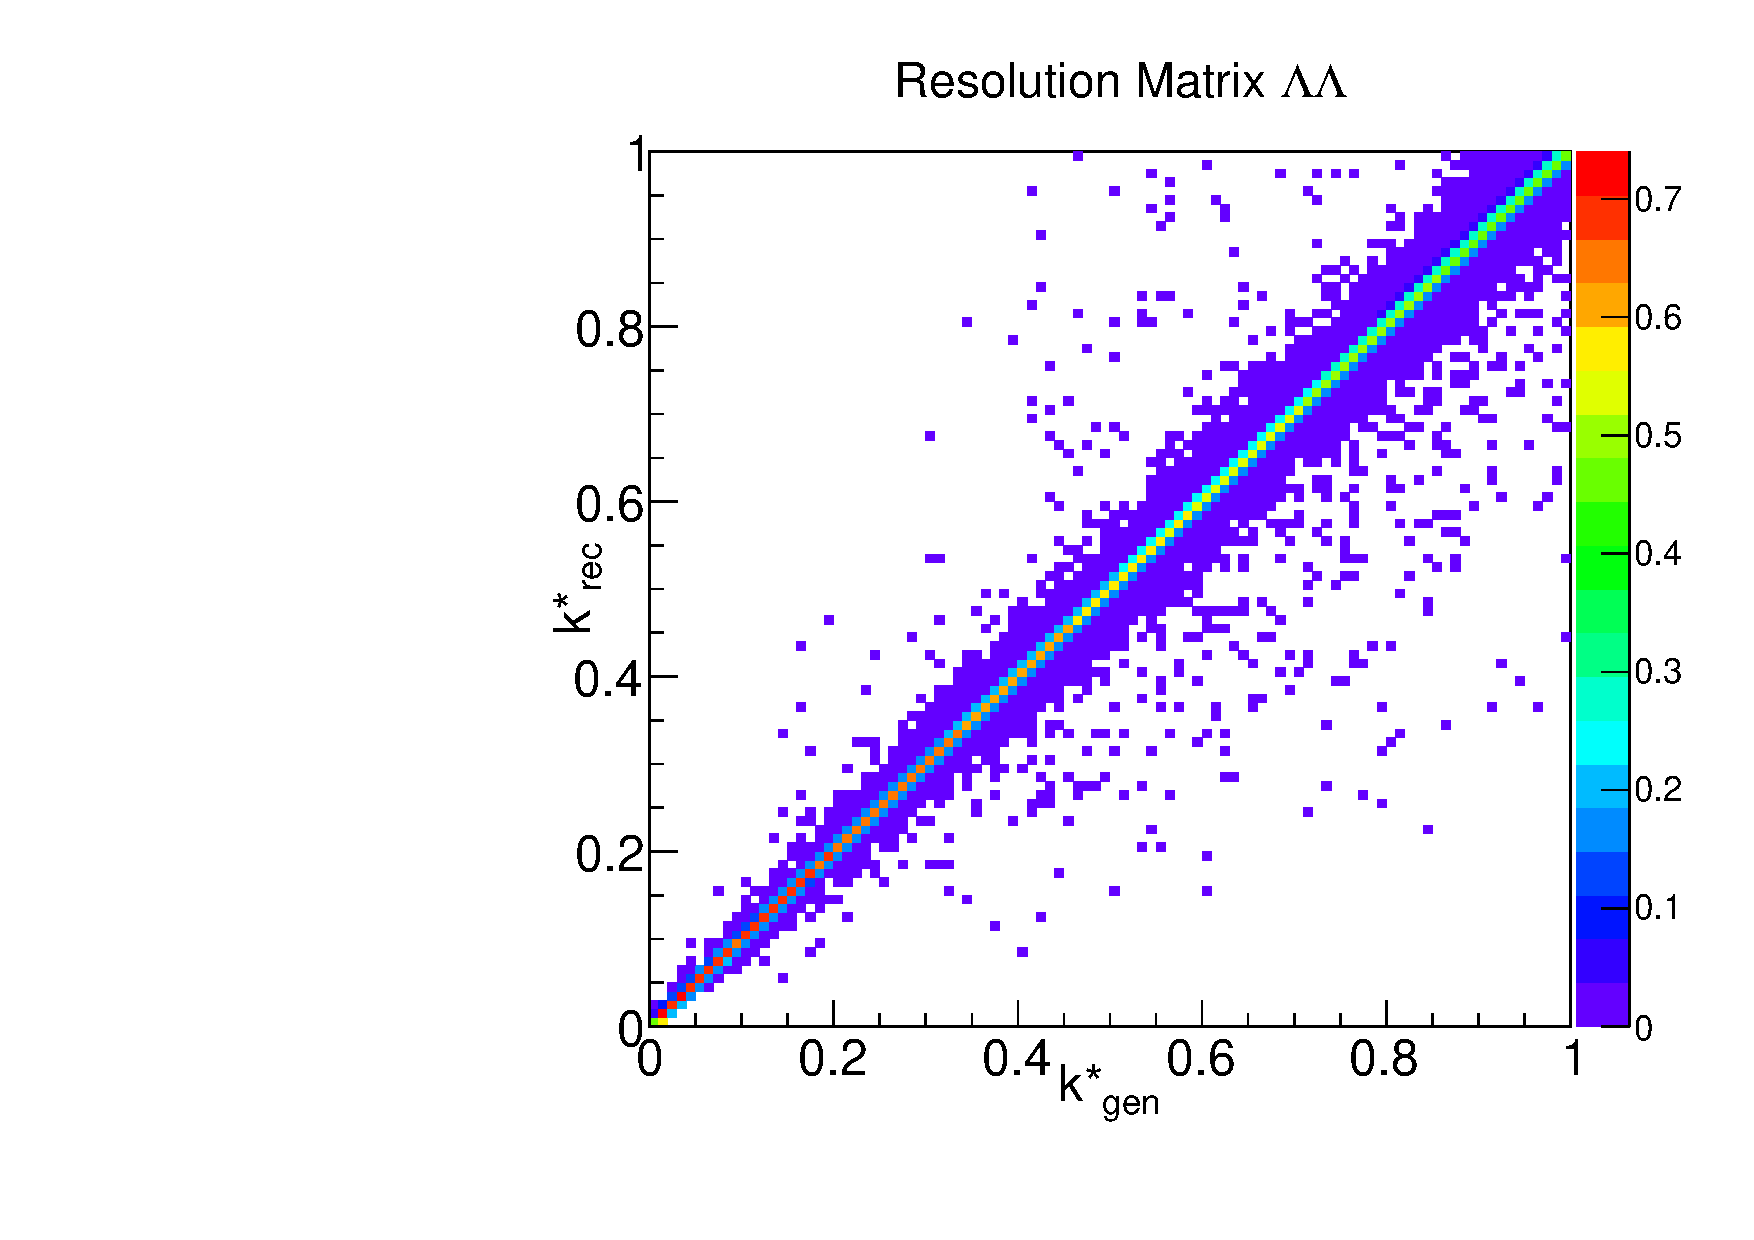
\includegraphics[width=18pc]{Figures/2016-07-19-ResMatrixLambdaLambda.pdf}
\end{minipage}\hspace{2pc}
\begin{minipage}{18pc}
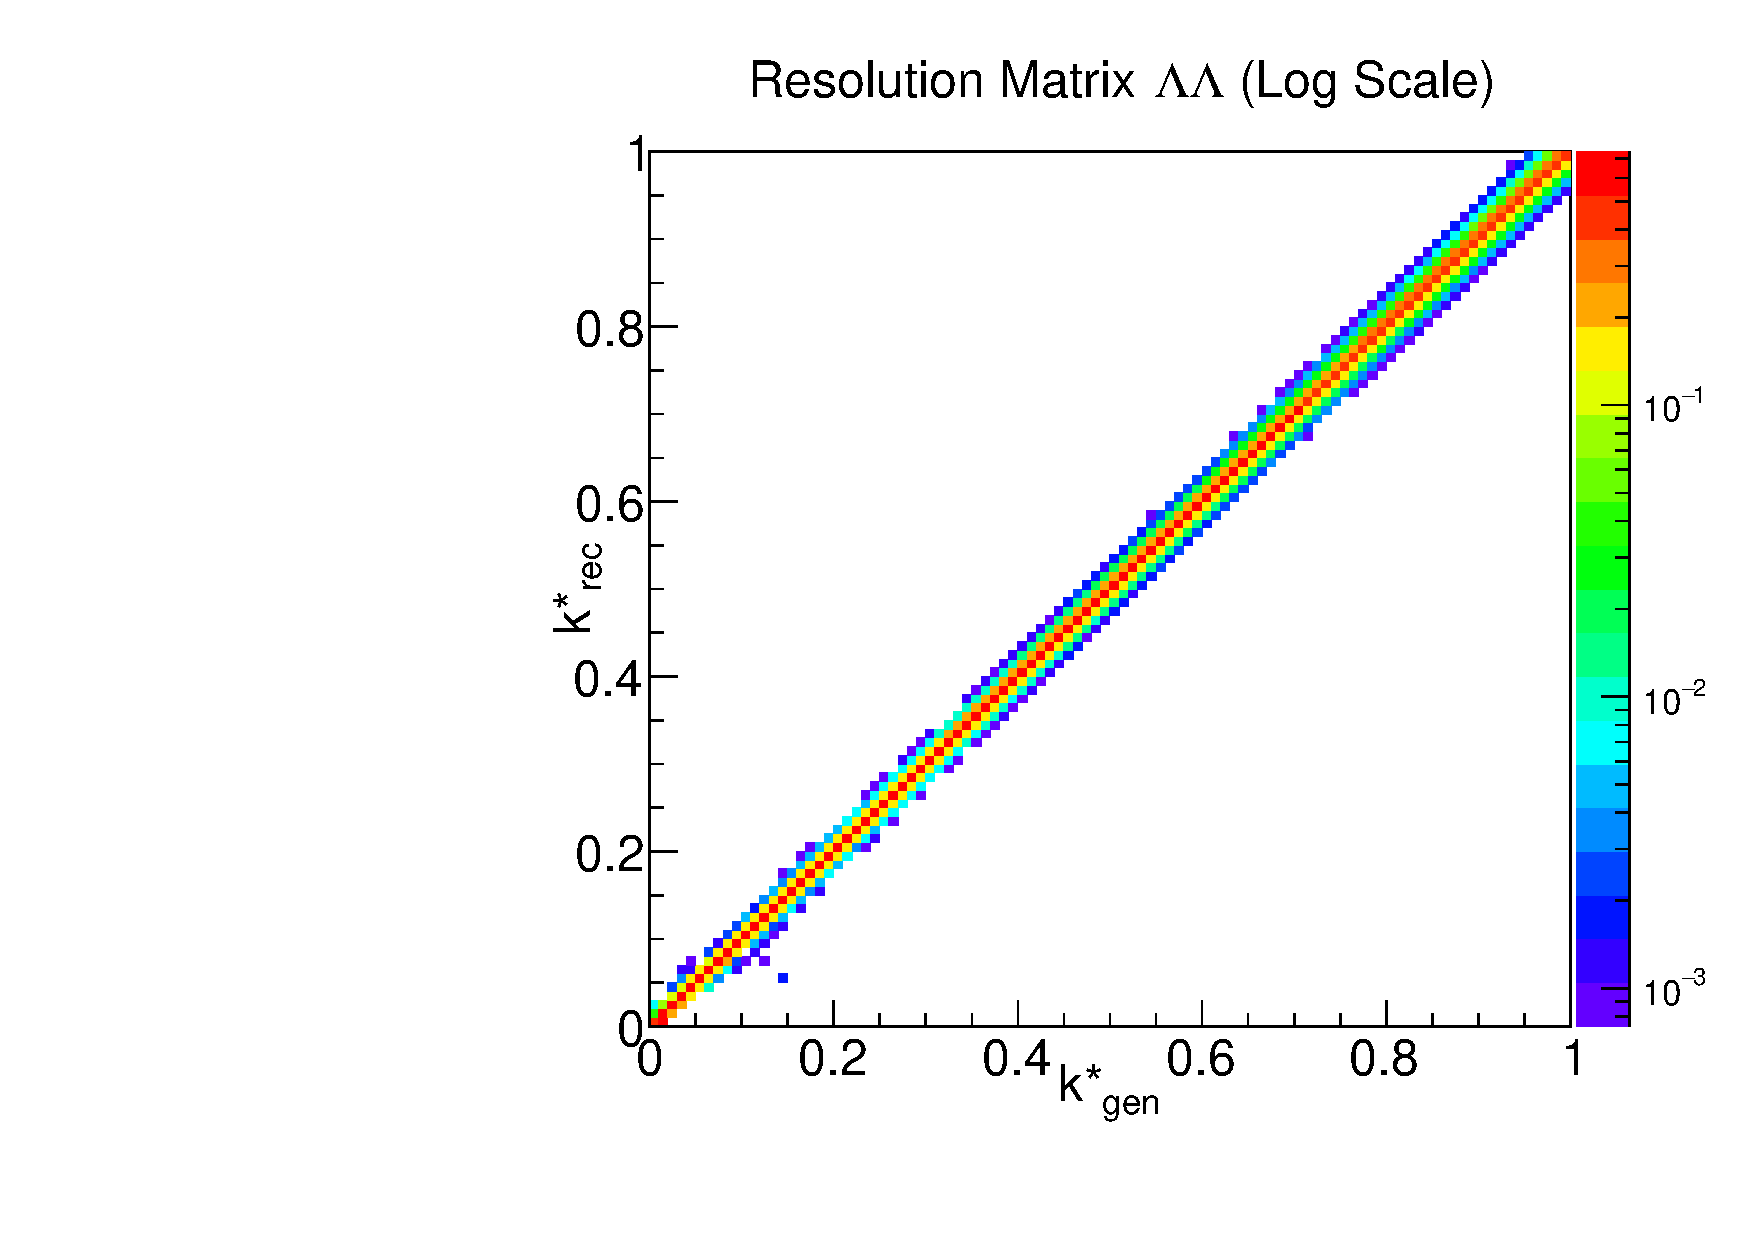
\includegraphics[width=18pc]{Figures/2016-07-19-ResMatrixLambdaLambdaLog.pdf}
\end{minipage} 
\caption[Momentum resolution matrices -- $\Lambda\Lambda$]{\label{fig:MomResLL} Momentum resolution matrices for $\Lambda\Lambda$. In the log scale plot (right), one can see tha the resolution smearing is very narrow --- most pairs have their $k^*$ shifted by no more than one or two bins.}
\end{figure}

\begin{figure}[h]
\begin{minipage}{18pc}
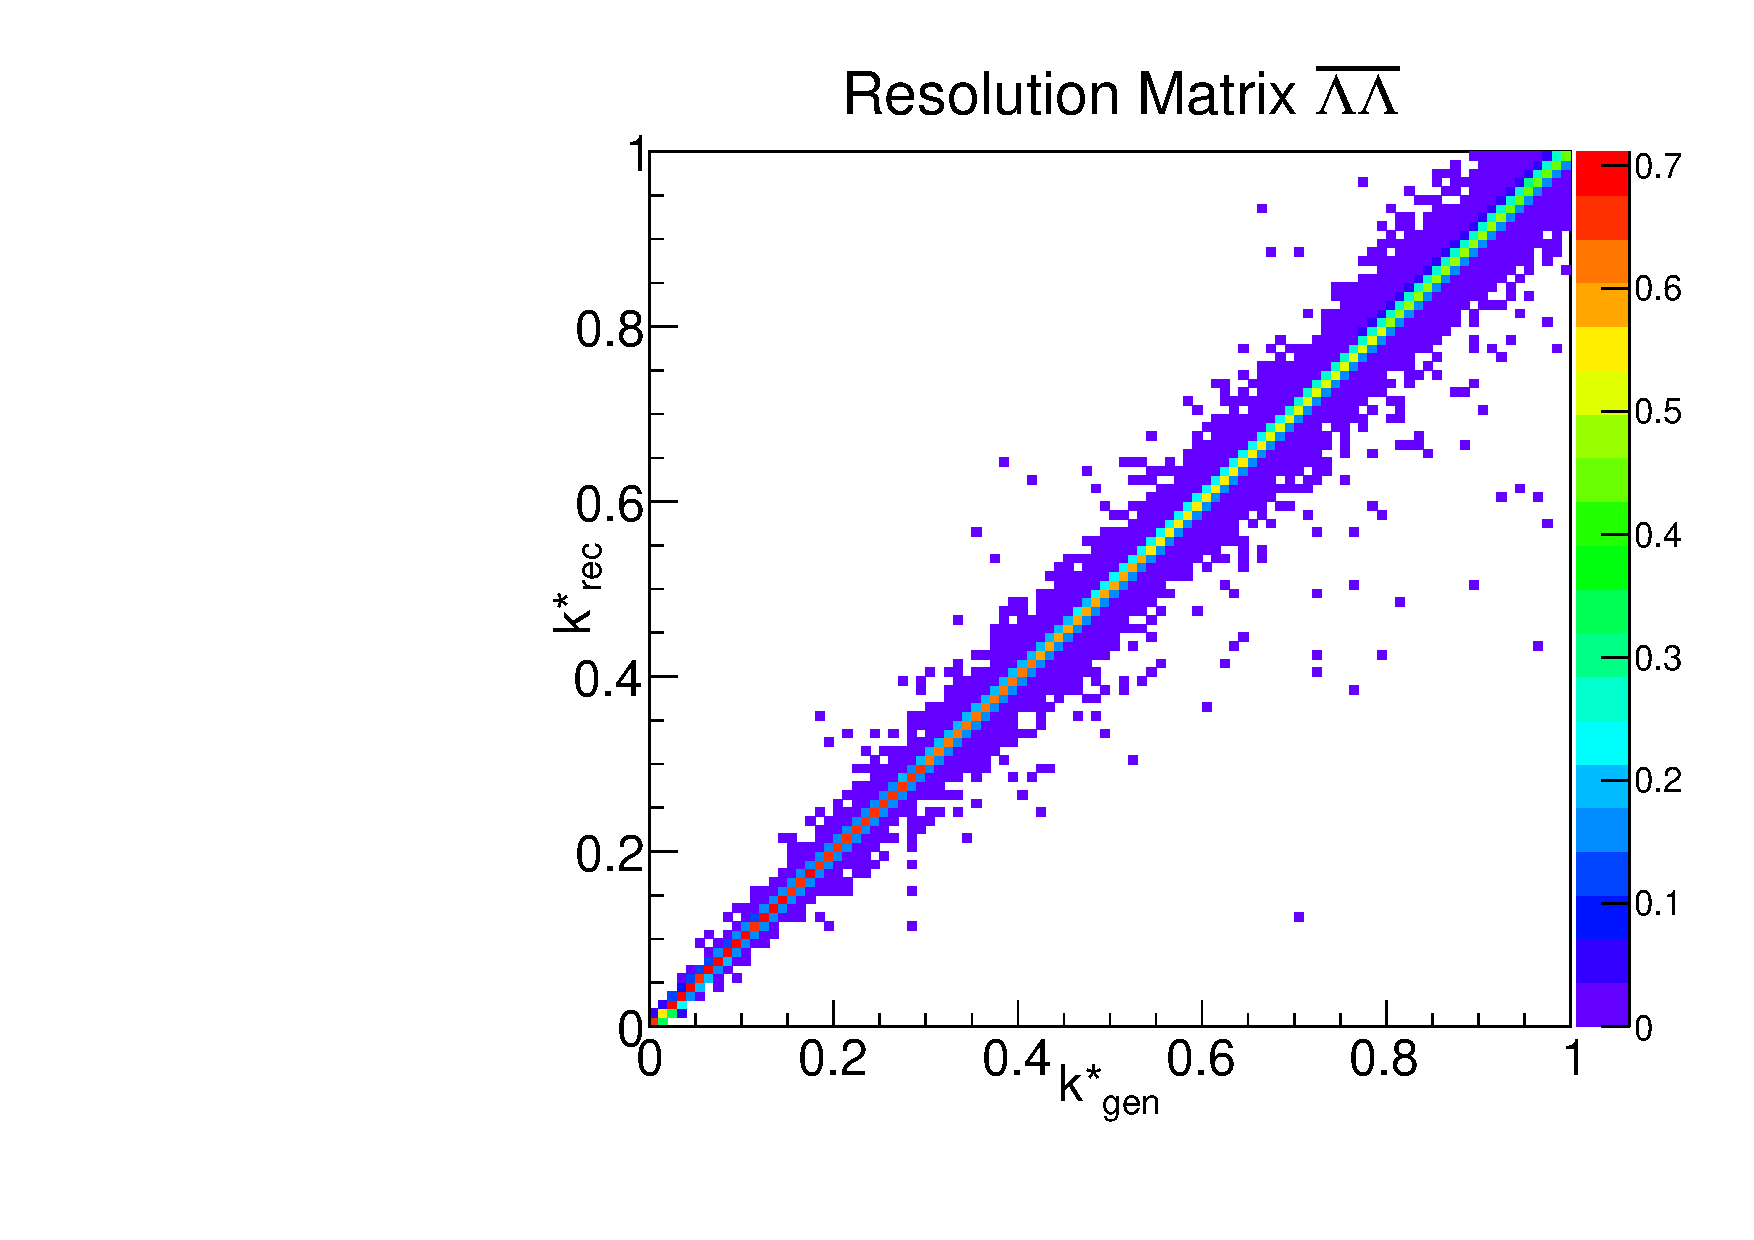
\includegraphics[width=18pc]{Figures/2016-07-19-ResMatrixAntiLambdaAntiLambda.pdf}
\end{minipage}\hspace{2pc}
\begin{minipage}{18pc}
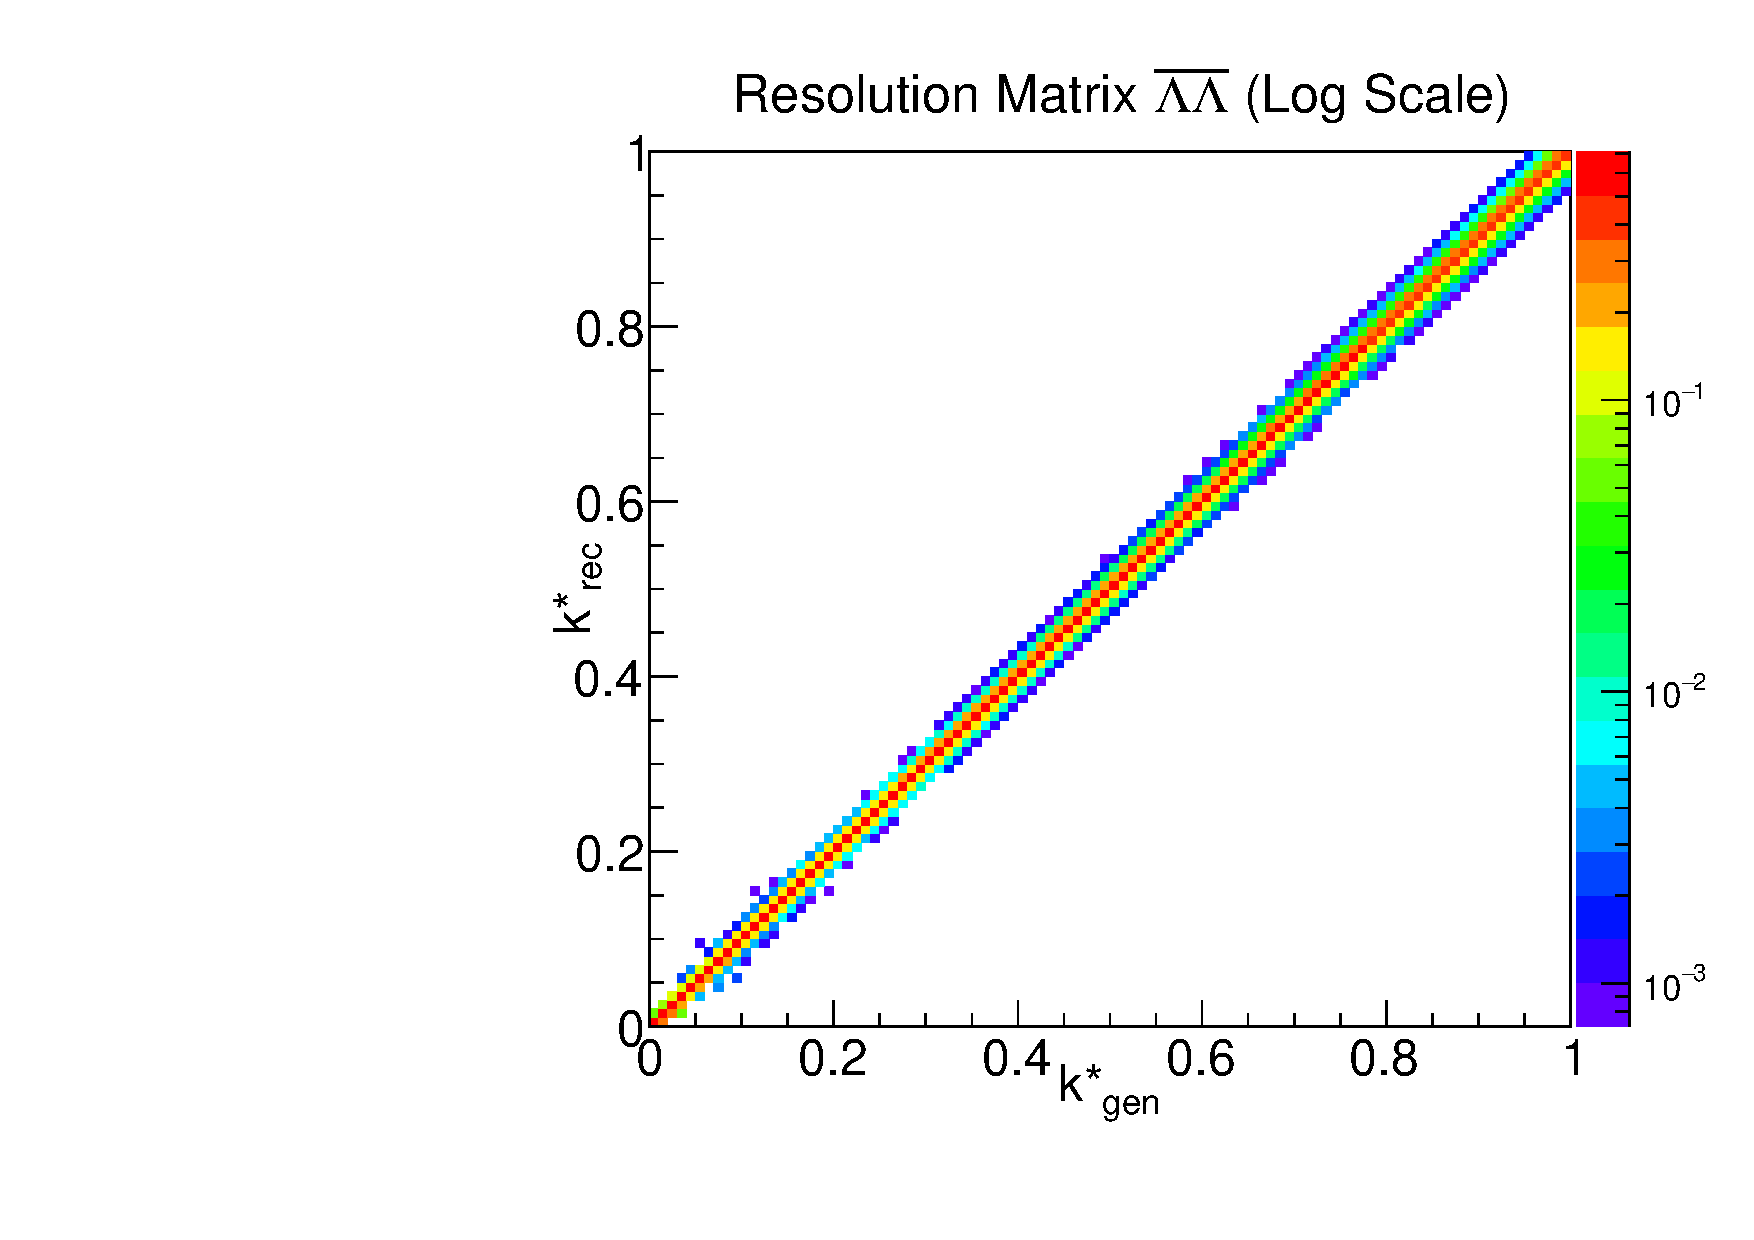
\includegraphics[width=18pc]{Figures/2016-07-19-ResMatrixAntiLambdaAntiLambdaLog.pdf}
\end{minipage} 
\caption[Momentum resolution matrices -- $\bar{\Lambda}\bar{\Lambda}$]{\label{fig:MomResAA} Momentum resolution matrices for $\bar{\Lambda}\bar{\Lambda}$. In the log scale plot (right), one can see tha the resolution smearing is very narrow --- most pairs have their $k^*$ shifted by no more than one or two bins.}
\end{figure}

\begin{figure}[h]
\begin{minipage}{18pc}
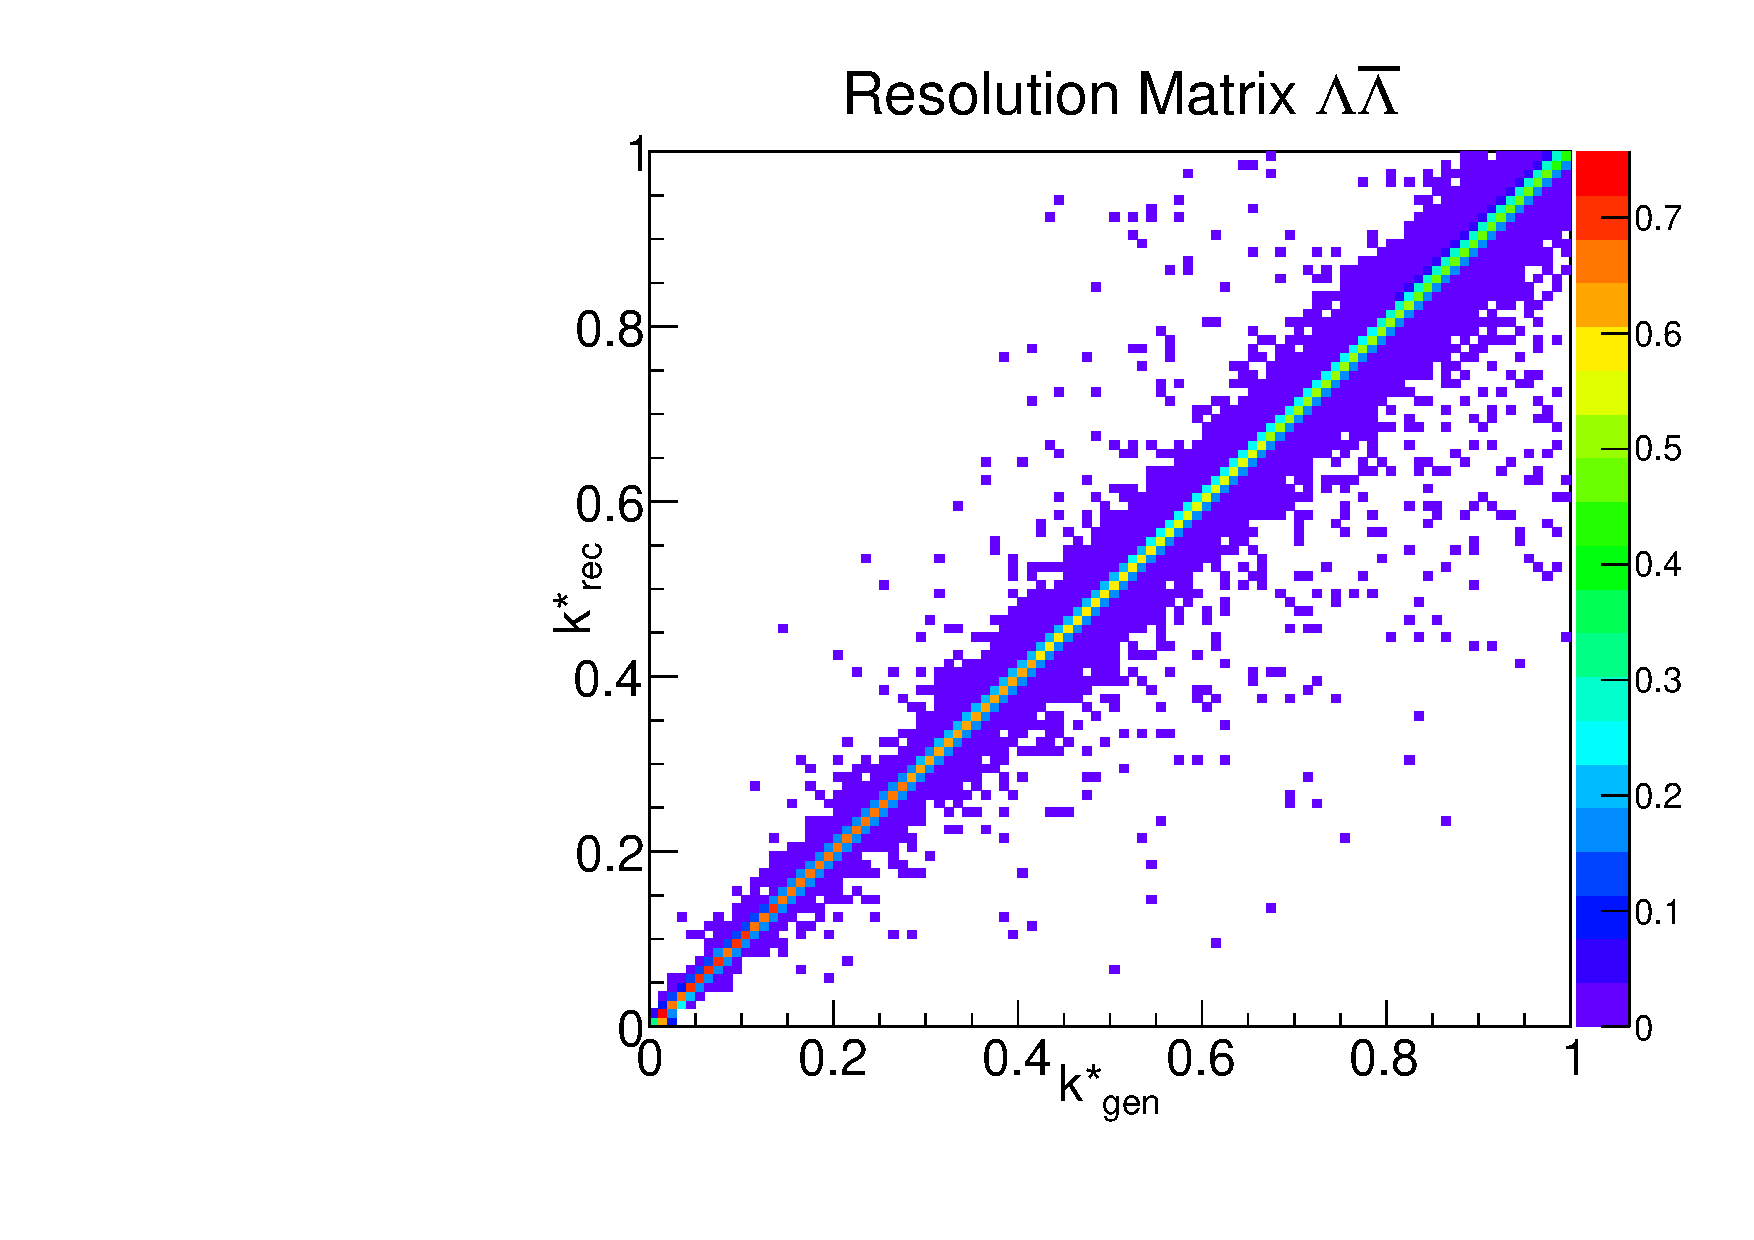
\includegraphics[width=18pc]{Figures/2016-07-19-ResMatrixLambdaAntiLambda.pdf}
\end{minipage}\hspace{2pc}
\begin{minipage}{18pc}
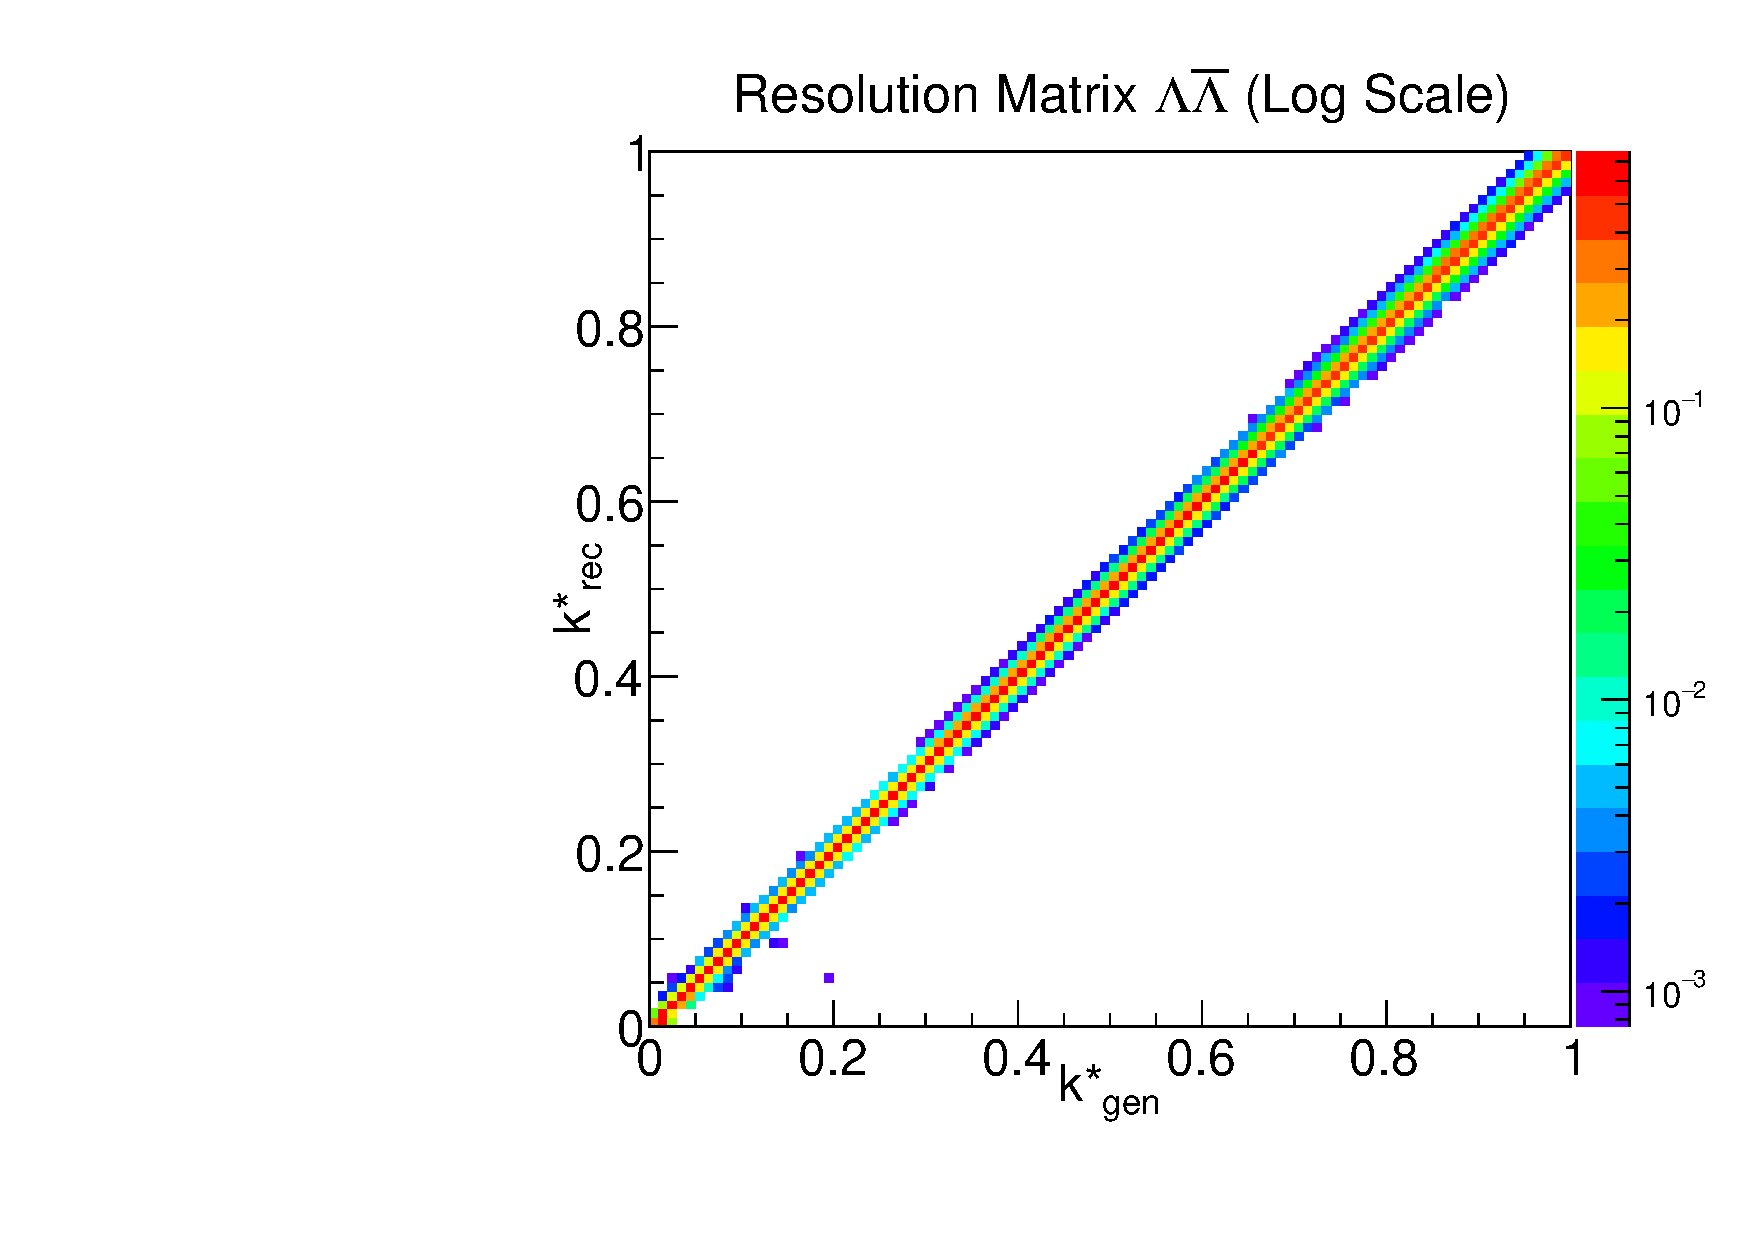
\includegraphics[width=18pc]{Figures/2016-07-19-ResMatrixLambdaAntiLambdaLog.pdf}
\end{minipage} 
\caption[Momentum resolution matrices -- $\Lambda\bar{\Lambda}$]{\label{fig:MomResLA} Momentum resolution matrices for $\Lambda\bar{\Lambda}$. In the log scale plot (right), one can see tha the resolution smearing is very narrow --- most pairs have their $k^*$ shifted by no more than one or two bins.}
\end{figure}

It is important to note that these histograms describe how a $k^*_\mathrm{gen}$ distribution can be smeared into a $k^*_\mathrm{recon}$ distribution, but not the reverse process (unsmearing).
Unsmearing would be described by the matrix inverse of these histograms.
Unfortunately, attempts to invert the matrices yield significant aliasing, and the results cannot be used.

That said, these momentum resolution matrices can be used to smear the theoretical prediction (i.e. the fit) from $k^*_\mathrm{gen}$--space into $k^*_\mathrm{recon}$--space using exactly the same procedure described above for residual correlation smearing:
\begin{equation}
\label{eq:MomResSmear}
C(k^*_{\mathrm{rec}}) \equiv \frac{\displaystyle\sum\limits_{k^*_{\mathrm{gen}}}M(k^*_{\mathrm{rec}},k^*_{\mathrm{gen}})C(k^*_{\mathrm{gen}})}{\displaystyle\sum\limits_{k^*_{\mathrm{gen}}}M(k^*_{\mathrm{rec}},k^*_{\mathrm{gen}})}.
\end{equation} 
Here, $M(k^*_{\mathrm{rec}},k^*_{\mathrm{gen}})$ is the momentum resolution smearing matrix.
One can perform this transformation on the fit function to ensure that both the data and the fit have the same smearing. 

There are two main benefits to treating the momentum resolution effects in this way. 
First, it is no longer necessary to run an iterative analysis (see Section \ref{sec:MomentumResCorrectionCF}). 
This method requires a one--time analysis of Monte Carlo data to produce the momentum resolution smearing matrix. 
Second, the resolution correction can be incorporated directly into the fit procedure as an intermediate step between calculating the fit function and taking the $\chi^2$ difference with the data.

\subsubsection{Smear matrices}
\label{sec:SmearMath}
Momentum resolution affects daughter tracks, and as such the primary or secondary nature of the parent $\Lambda$ is irrelevant.
Therefore, when smearing the fit function, momentum resolution smearing should be applied after residual correlation smearing. 
In fact, as both types of smearing are effectively forms of matrix algebra, the two smearing effects can be rolled together. 
In that case, $C(k^*_\mathrm{gen})$ in Eqn.\ \ref{eq:MomResSmear} is the theoretical correlation function for some pair type expressed in terms of $k^*_{\Lambda\Lambda}$, as given by Eqn.\ \ref{eq:ResCorSmear}.

Combined together, they give (in the case of $\Lambda\Sigma$ feeddown)
\begin{equation}
C_{\Lambda\Sigma}(k^{*\Lambda\Lambda}_{\mathrm{rec}}) \equiv \frac{\displaystyle\sum\limits_{k^{*\Lambda\Lambda}_{\mathrm{gen}}}M(k^{*\Lambda\Lambda}_{\mathrm{rec}},k^{*\Lambda\Lambda}_{\mathrm{gen}})
 \frac{\displaystyle\sum\limits_{k^{*\Lambda\Sigma}_{\mathrm{gen}}}T(k^{*\Lambda\Lambda}_\mathrm{gen},k^{*\Lambda\Sigma}_{\mathrm{gen}})C_{\Lambda\Sigma}(k^{*\Lambda\Sigma}_{\mathrm{gen}})}{\displaystyle\sum\limits_{k^{*\Lambda\Sigma}_{\mathrm{gen}}}T(k^{*\Lambda\Lambda}_\mathrm{gen},k^{*\Lambda\Sigma}_{\mathrm{gen}})}
}{\displaystyle\sum\limits_{k^{*\Lambda\Lambda}_{\mathrm{gen}}}M(k^{*\Lambda\Lambda}_{\mathrm{rec}},k^{*\Lambda\Lambda}_{\mathrm{gen}})}.
\end{equation}

This becomes much cleaner if we introduce the partially-normalized (i.e.\ along one axis) matrices
\begin{equation}
\tilde{M}(k^*_{\mathrm{rec}},k^*_{\mathrm{gen}}) \equiv \frac{M(k^*_{\mathrm{rec}},k^*_{\mathrm{gen}})}{\displaystyle\sum\limits_{k^*_{\mathrm{gen}}}M(k^*_{\mathrm{rec}},k^*_{\mathrm{gen}})}
\end{equation}
and
\begin{equation}
\tilde{T}(k^*_{\Lambda\Lambda},k^*_{\Lambda\Sigma}) \equiv \frac{T(k^*_{\Lambda\Lambda},k^*_{\Lambda\Sigma})}{\displaystyle\sum\limits_{k^*_{\Lambda\Sigma}}T(k^*_{\Lambda\Lambda},k^*_{\Lambda\Sigma})}.
\end{equation}
Then we get the more compact
\begin{equation}
C_{\Lambda\Sigma}(k^{*\Lambda\Lambda}_{\mathrm{rec}}) = \displaystyle\sum\limits_{k^{*\Lambda\Lambda}_{\mathrm{gen}}}\tilde{M}(k^{*\Lambda\Lambda}_{\mathrm{rec}},k^{*\Lambda\Lambda}_{\mathrm{gen}})\displaystyle\sum\limits_{k^{*\Lambda\Sigma}_{\mathrm{gen}}}\tilde{T}(k^{*\Lambda\Lambda}_\mathrm{gen},k^{*\Lambda\Sigma}_{\mathrm{gen}})C_{\Lambda\Sigma}(k^{*\Lambda\Sigma}_{\mathrm{gen}})
\end{equation}
We can contract the $k^{*\Lambda\Lambda}_\mathrm{gen}$ indices to get
\begin{equation}
\label{eq:FullSmearing}
C_{\Lambda\Sigma}(k^{*\Lambda\Lambda}_{\mathrm{rec}}) = \displaystyle\sum\limits_{k^{*\Lambda\Sigma}_{\mathrm{gen}}}S(k^{*\Lambda\Lambda}_{\mathrm{rec}},k^{*\Lambda\Sigma}_{\mathrm{gen}})C_{\Lambda\Sigma}(k^{*\Lambda\Sigma}_{\mathrm{gen}}),
\end{equation}
where 
\begin{equation}
\label{eq:SmearMatrix}
S(k^{*\Lambda\Lambda}_{\mathrm{rec}},k^{*\Lambda\Sigma}_{\mathrm{gen}}) \equiv \displaystyle\sum\limits_{k^{*\Lambda\Lambda}_{\mathrm{gen}}}\tilde{M}(k^{*\Lambda\Lambda}_{\mathrm{rec}},k^{*\Lambda\Lambda}_{\mathrm{gen}})\tilde{T}(k^{*\Lambda\Lambda}_\mathrm{gen},k^{*\Lambda\Sigma}_{\mathrm{gen}}).
\end{equation}

There are multiple residual correlation transform matrices (one for each pair that decays into $\Lambda\Lambda$), and a corresponding number of full smearing matrices $S$ defined by Eqn.\ \ref{eq:SmearMatrix}.
For consistency, we also treat the momentum resolution smearing of primary $\Lambda\Lambda$ as a smearing matrix, though here the residual correlation matrix $\tilde{T}$ would be the identity matrix. 
Figures \ref{fig:SmearLLAA}--\ref{fig:SmearXiCXi0LA} show the full smear matrices.

\begin{figure}[h]
\begin{minipage}{18pc}
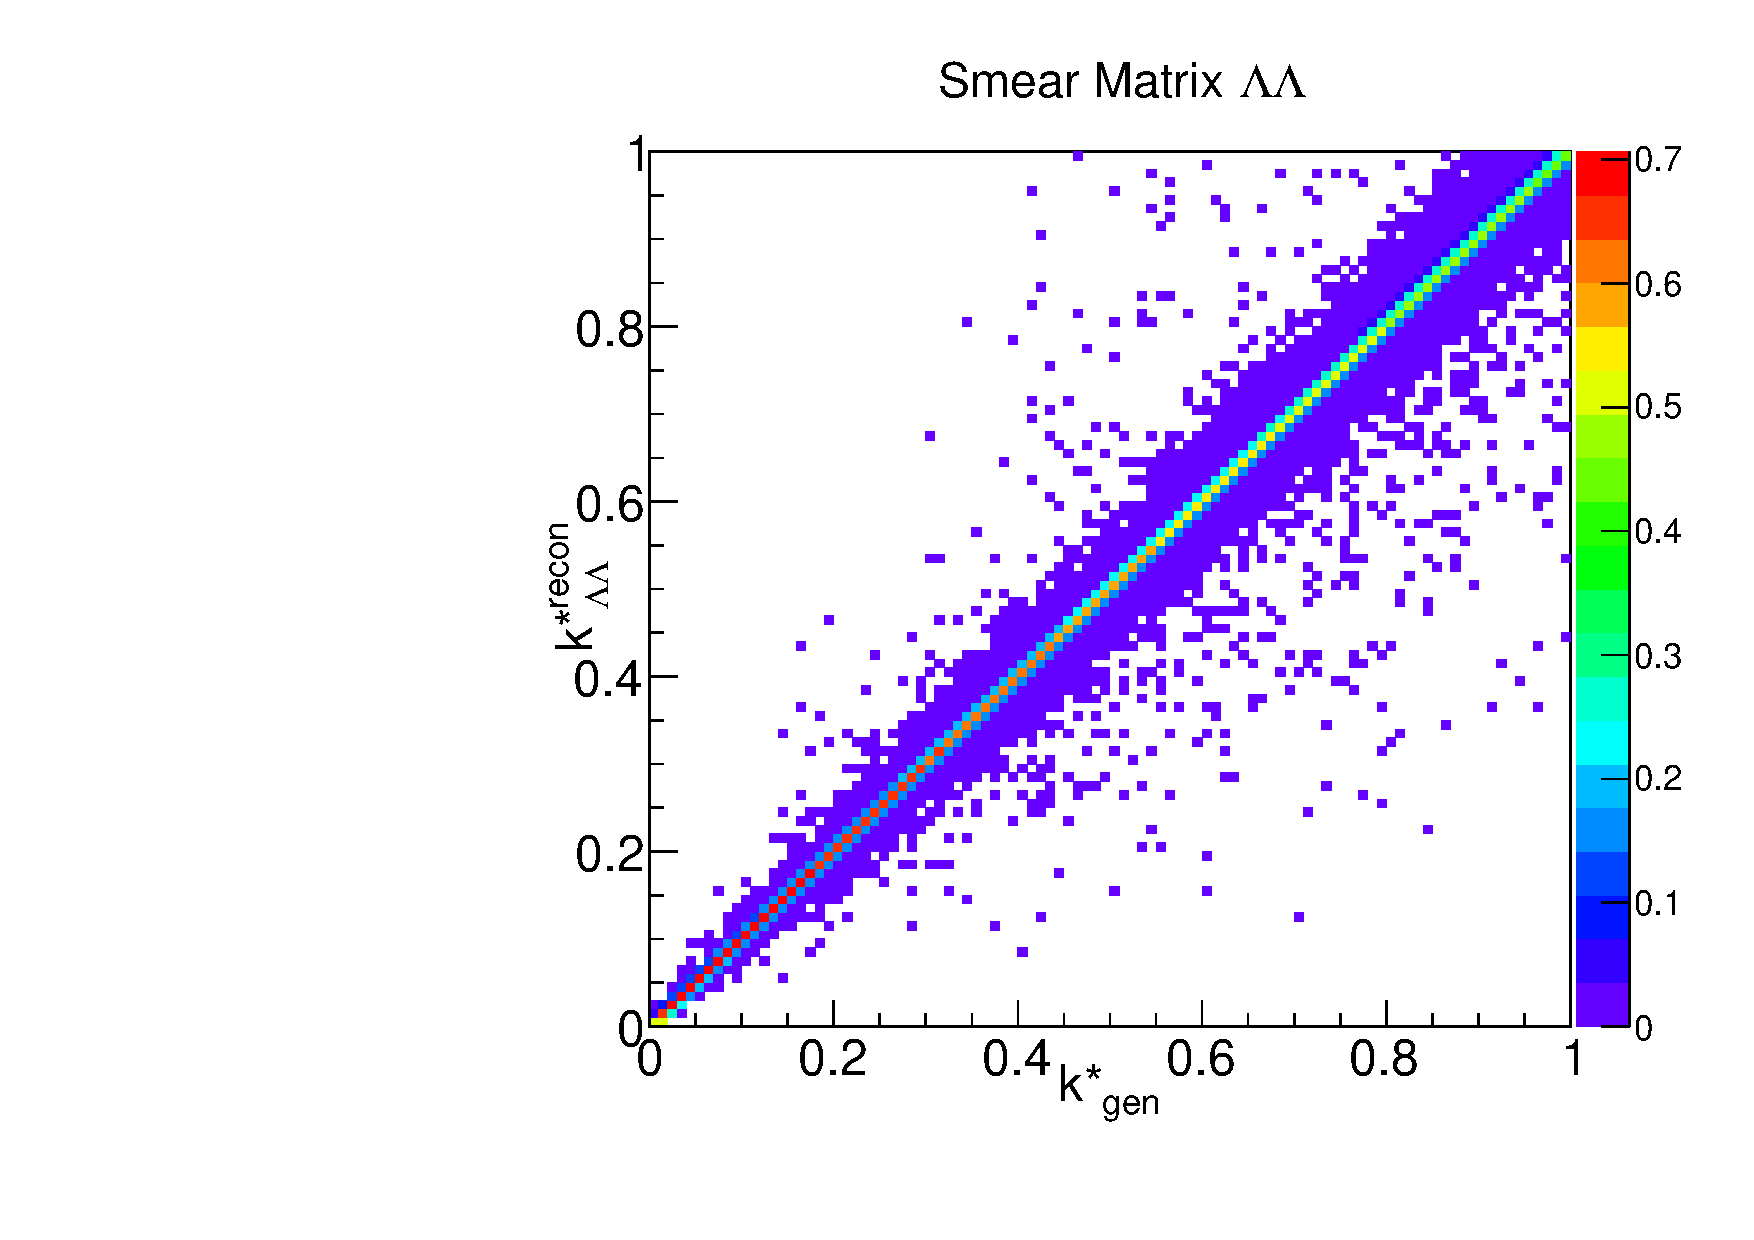
\includegraphics[width=18pc]{Figures/SmearMatrices/2016-7-19-SmearMatrixLambdaLambdaNormLLAA.pdf}
\end{minipage}\hspace{2pc}
\begin{minipage}{18pc}
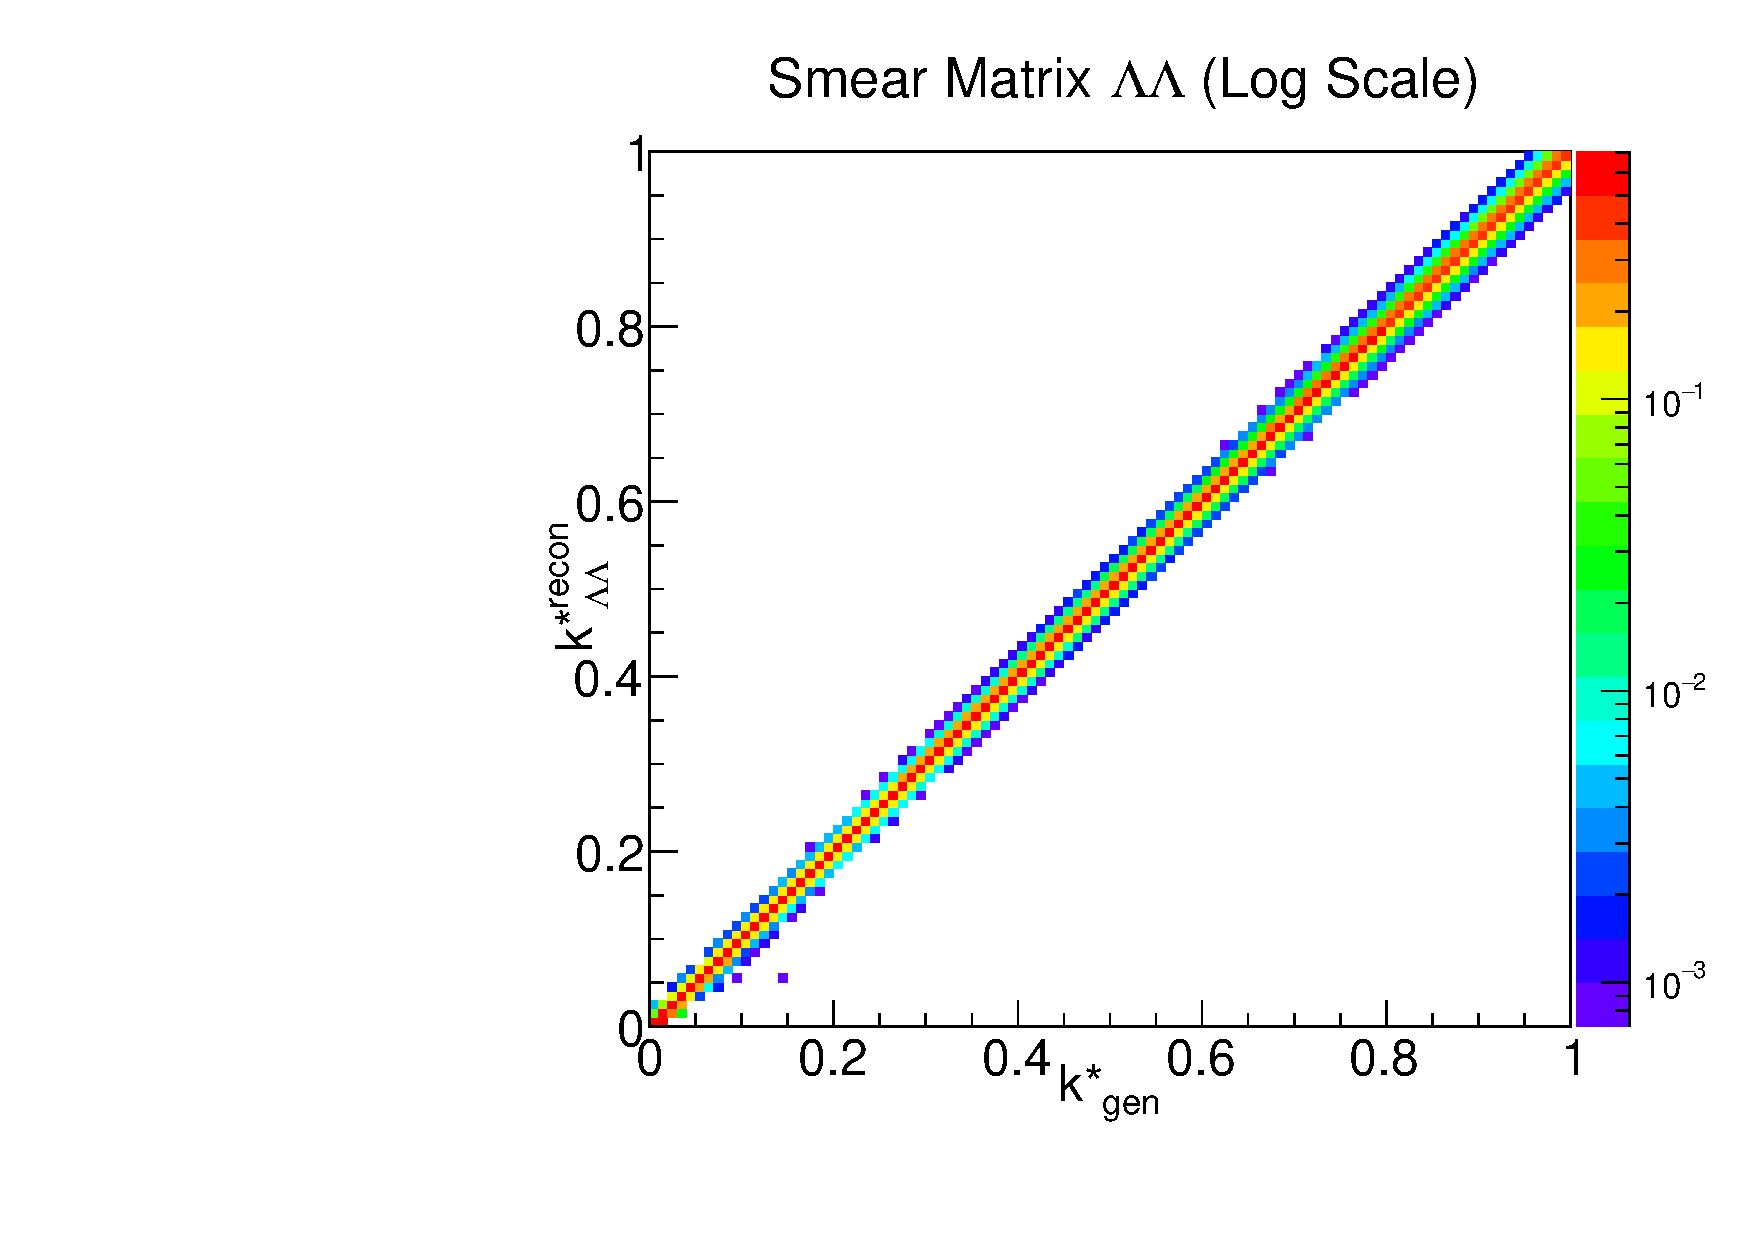
\includegraphics[width=18pc]{Figures/SmearMatrices/2016-7-19-SmearMatrixLambdaLambdaNormLLAALog.pdf}
\end{minipage} 
\caption[Smear matrix -- $\Lambda\Lambda$]{\label{fig:SmearLLAA} 
Smear matrix used for both $\Lambda\Lambda$ and $\bar{\Lambda}\bar{\Lambda}$. As the residual correlation matrix for primary $\Lambda\Lambda$ pairs is the identity matrix, these plots are identical to the plots in Figure \ref{fig:MomResLL}.}
\end{figure}

\begin{figure}[h]
\begin{minipage}{18pc}
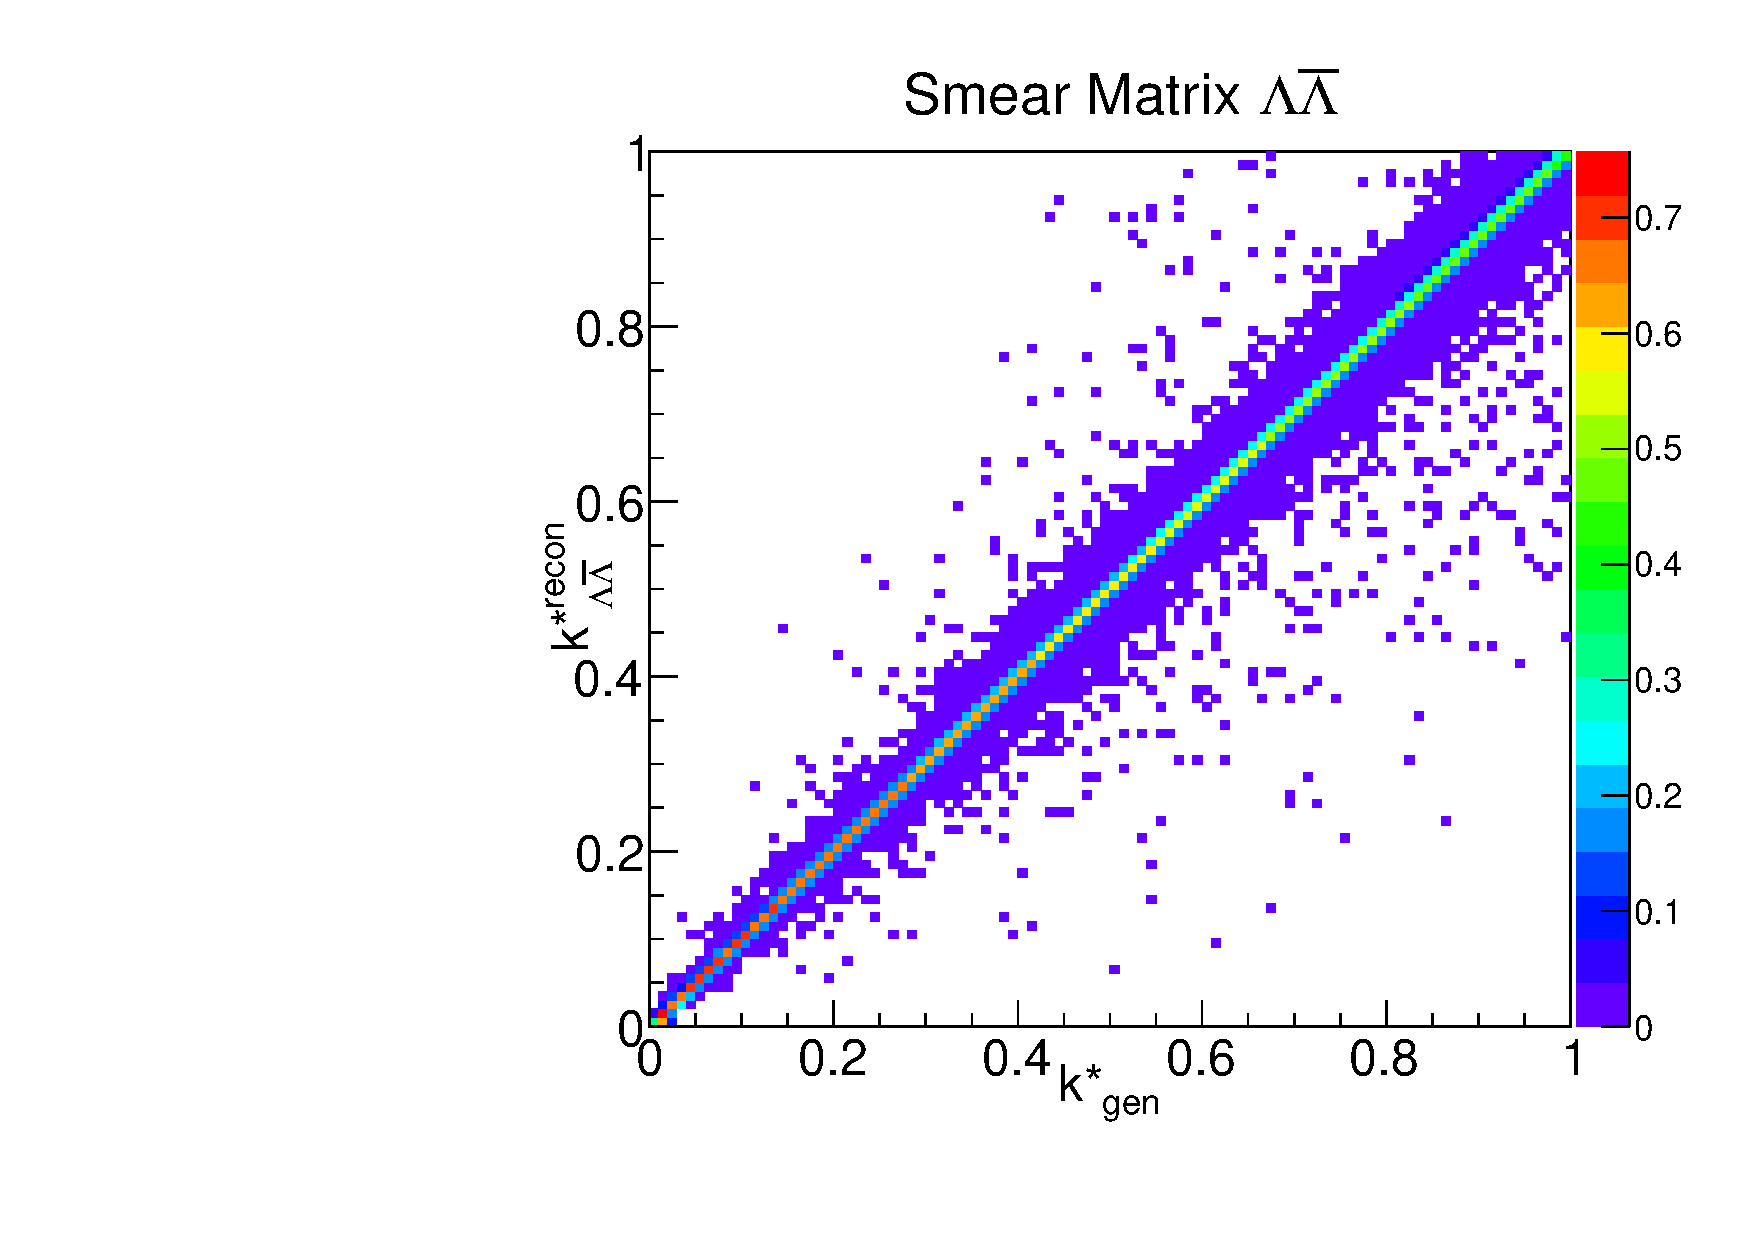
\includegraphics[width=18pc]{Figures/SmearMatrices/2016-7-19-SmearMatrixLambdaLambdaNormLA.pdf}
\end{minipage}\hspace{2pc}
\begin{minipage}{18pc}
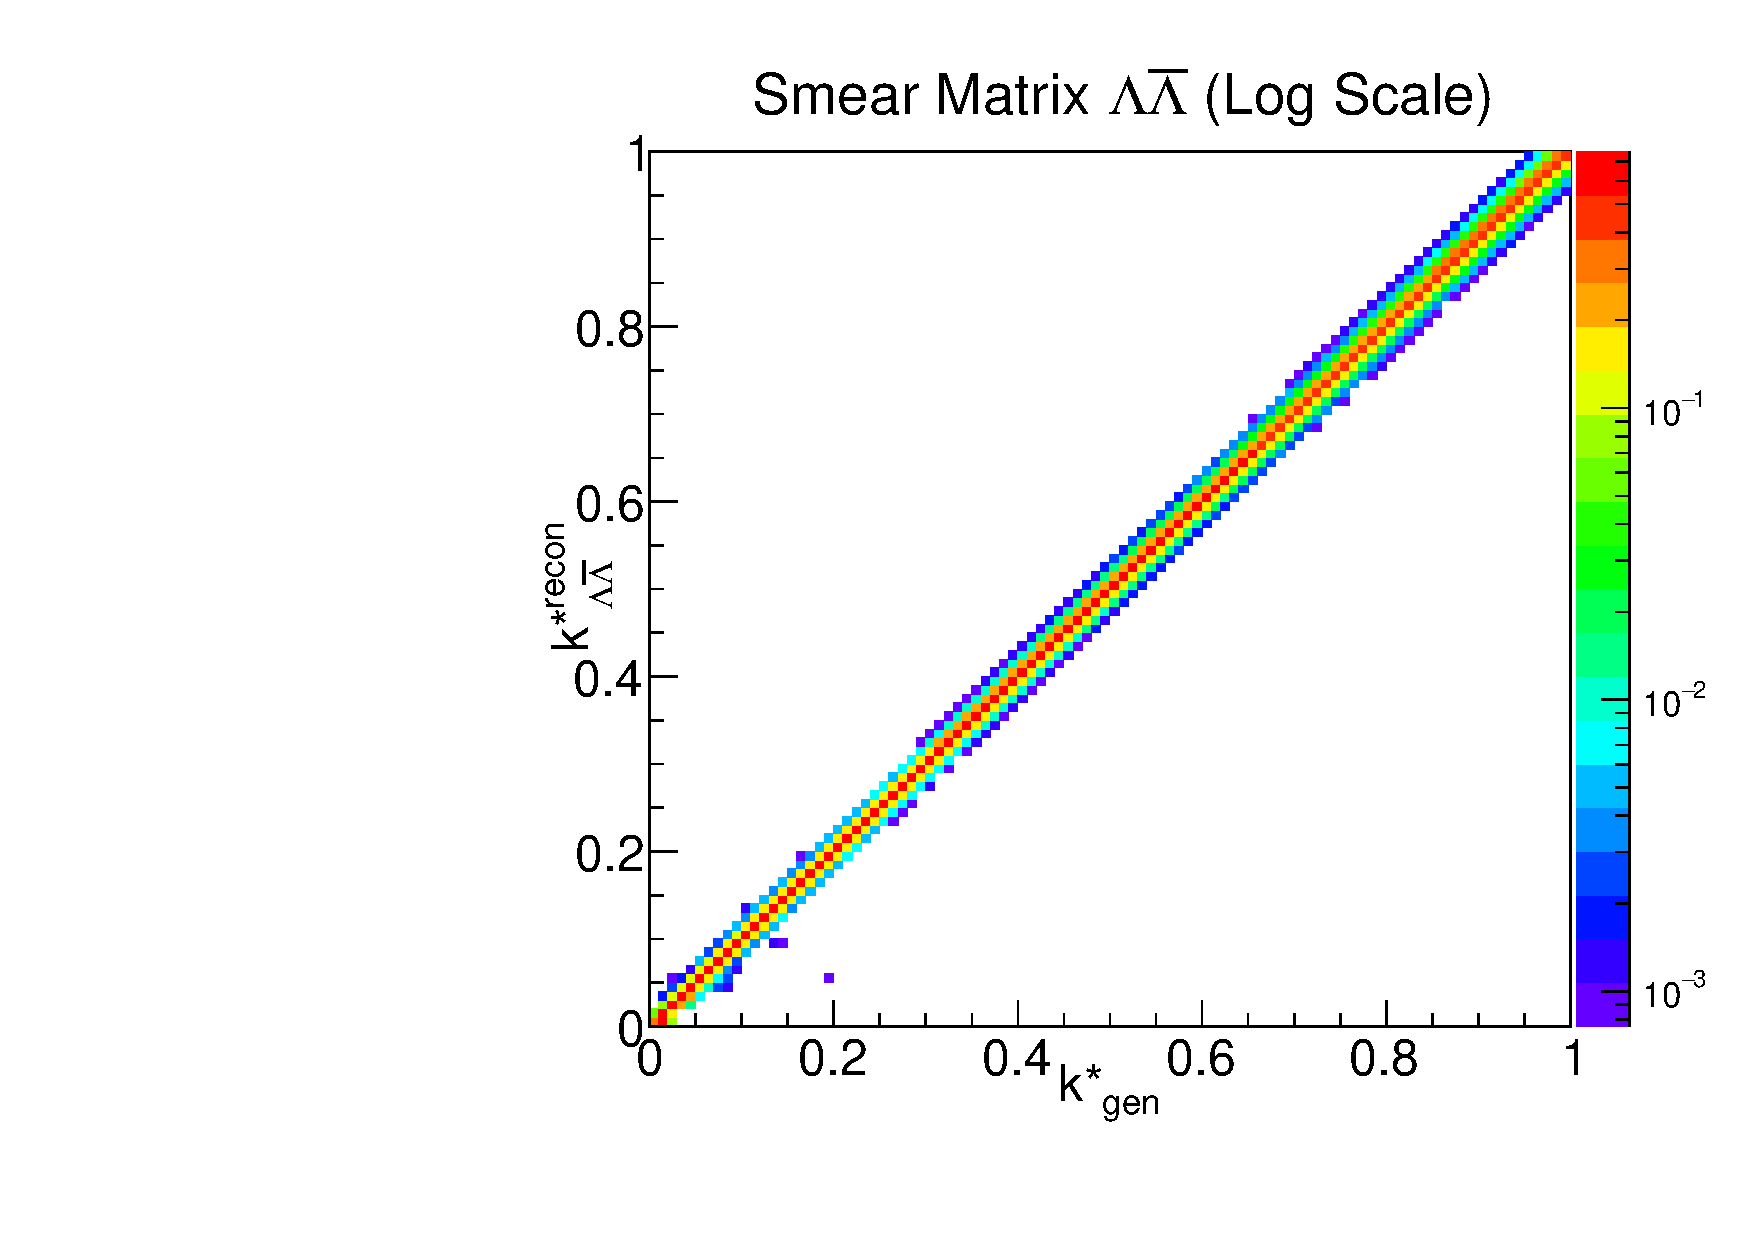
\includegraphics[width=18pc]{Figures/SmearMatrices/2016-7-19-SmearMatrixLambdaLambdaNormLALog.pdf}
\end{minipage} 
\caption[Smear matrix -- $\Lambda\bar{\Lambda}$]{\label{fig:SmearLA} 
Smear matrix for $\Lambda\bar{\Lambda}$. As the residual correlation matrix for primary $\Lambda\bar{\Lambda}$ pairs is the identity matrix, these plots are identical to the plots in Figure \ref{fig:MomResLA}.}
\end{figure}

\begin{figure}[h]
\begin{minipage}{18pc}
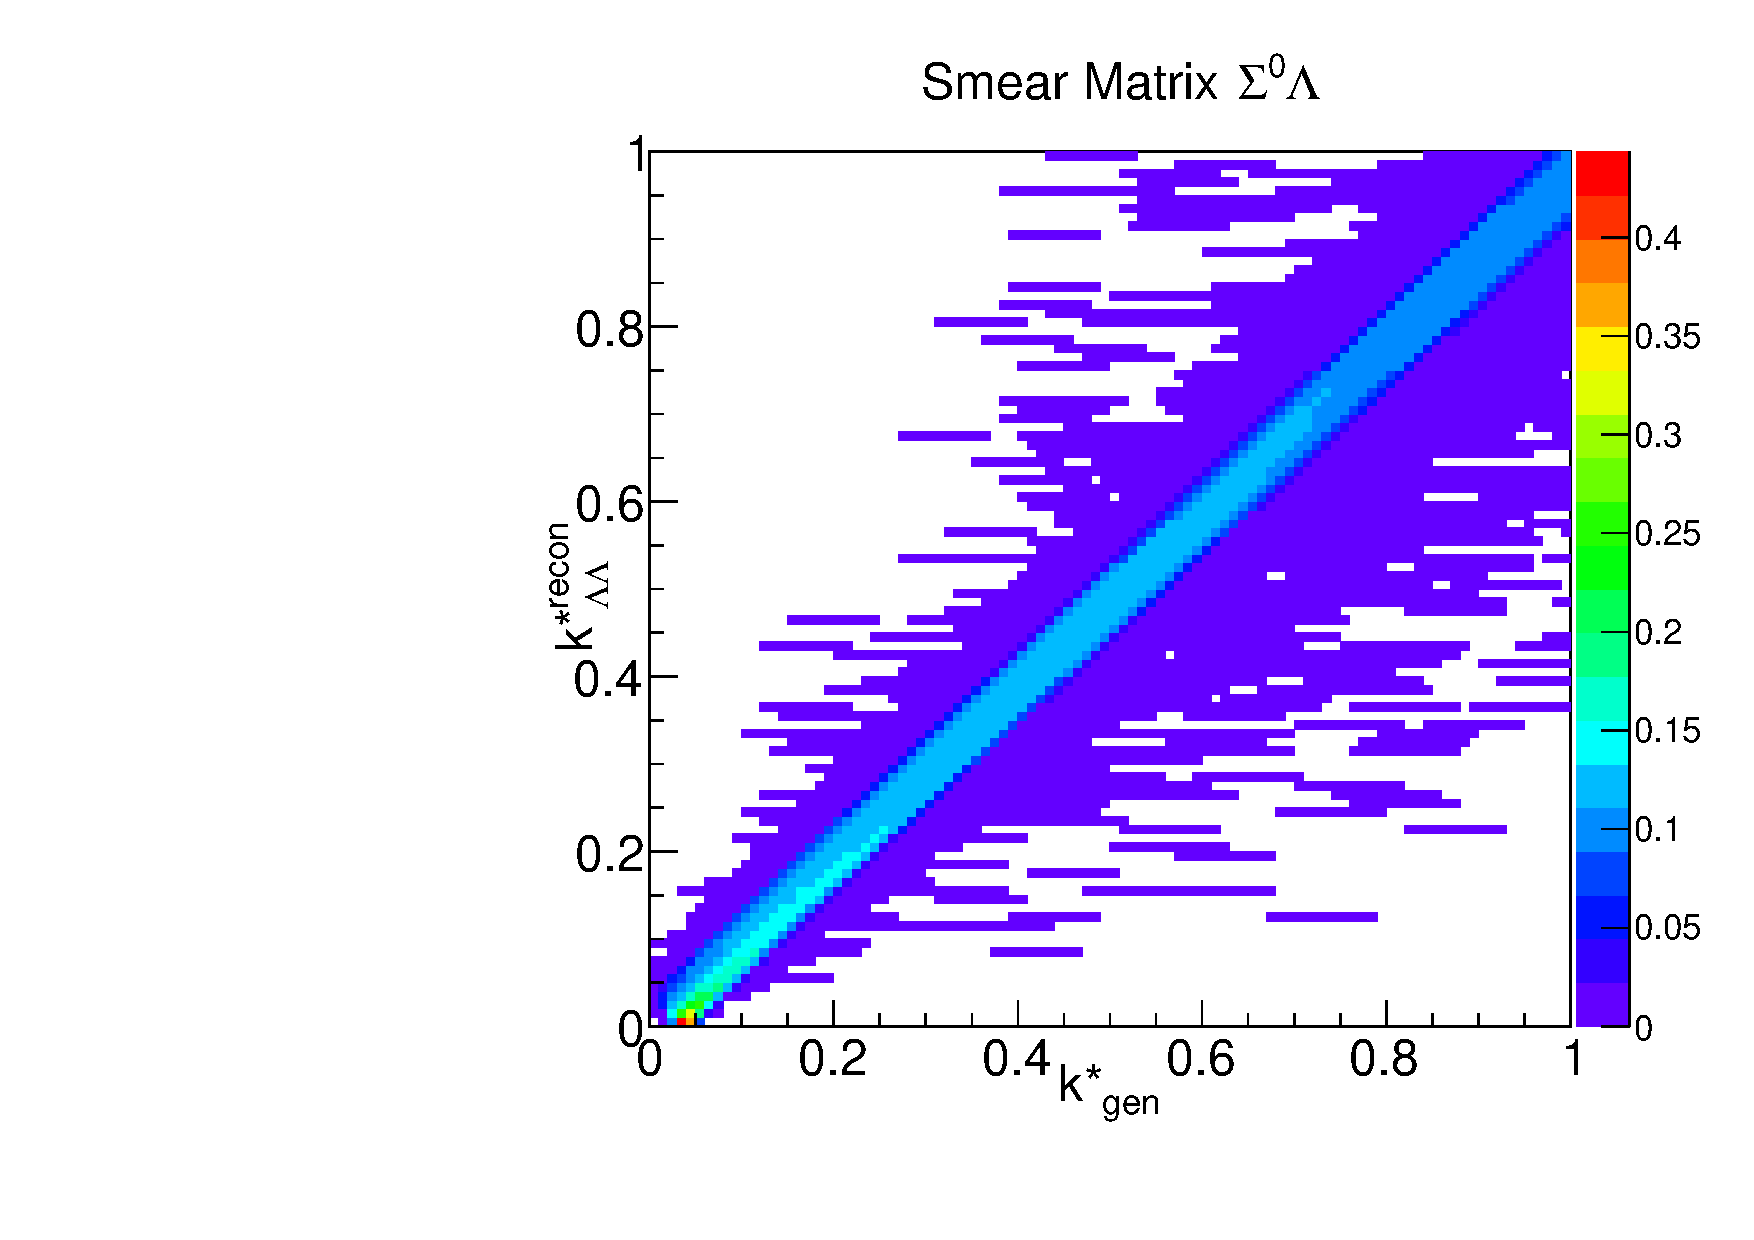
\includegraphics[width=18pc]{Figures/SmearMatrices/2016-7-19-SmearMatrixSigmaLambdaNormLLAA.pdf}
\end{minipage}\hspace{2pc}
\begin{minipage}{18pc}
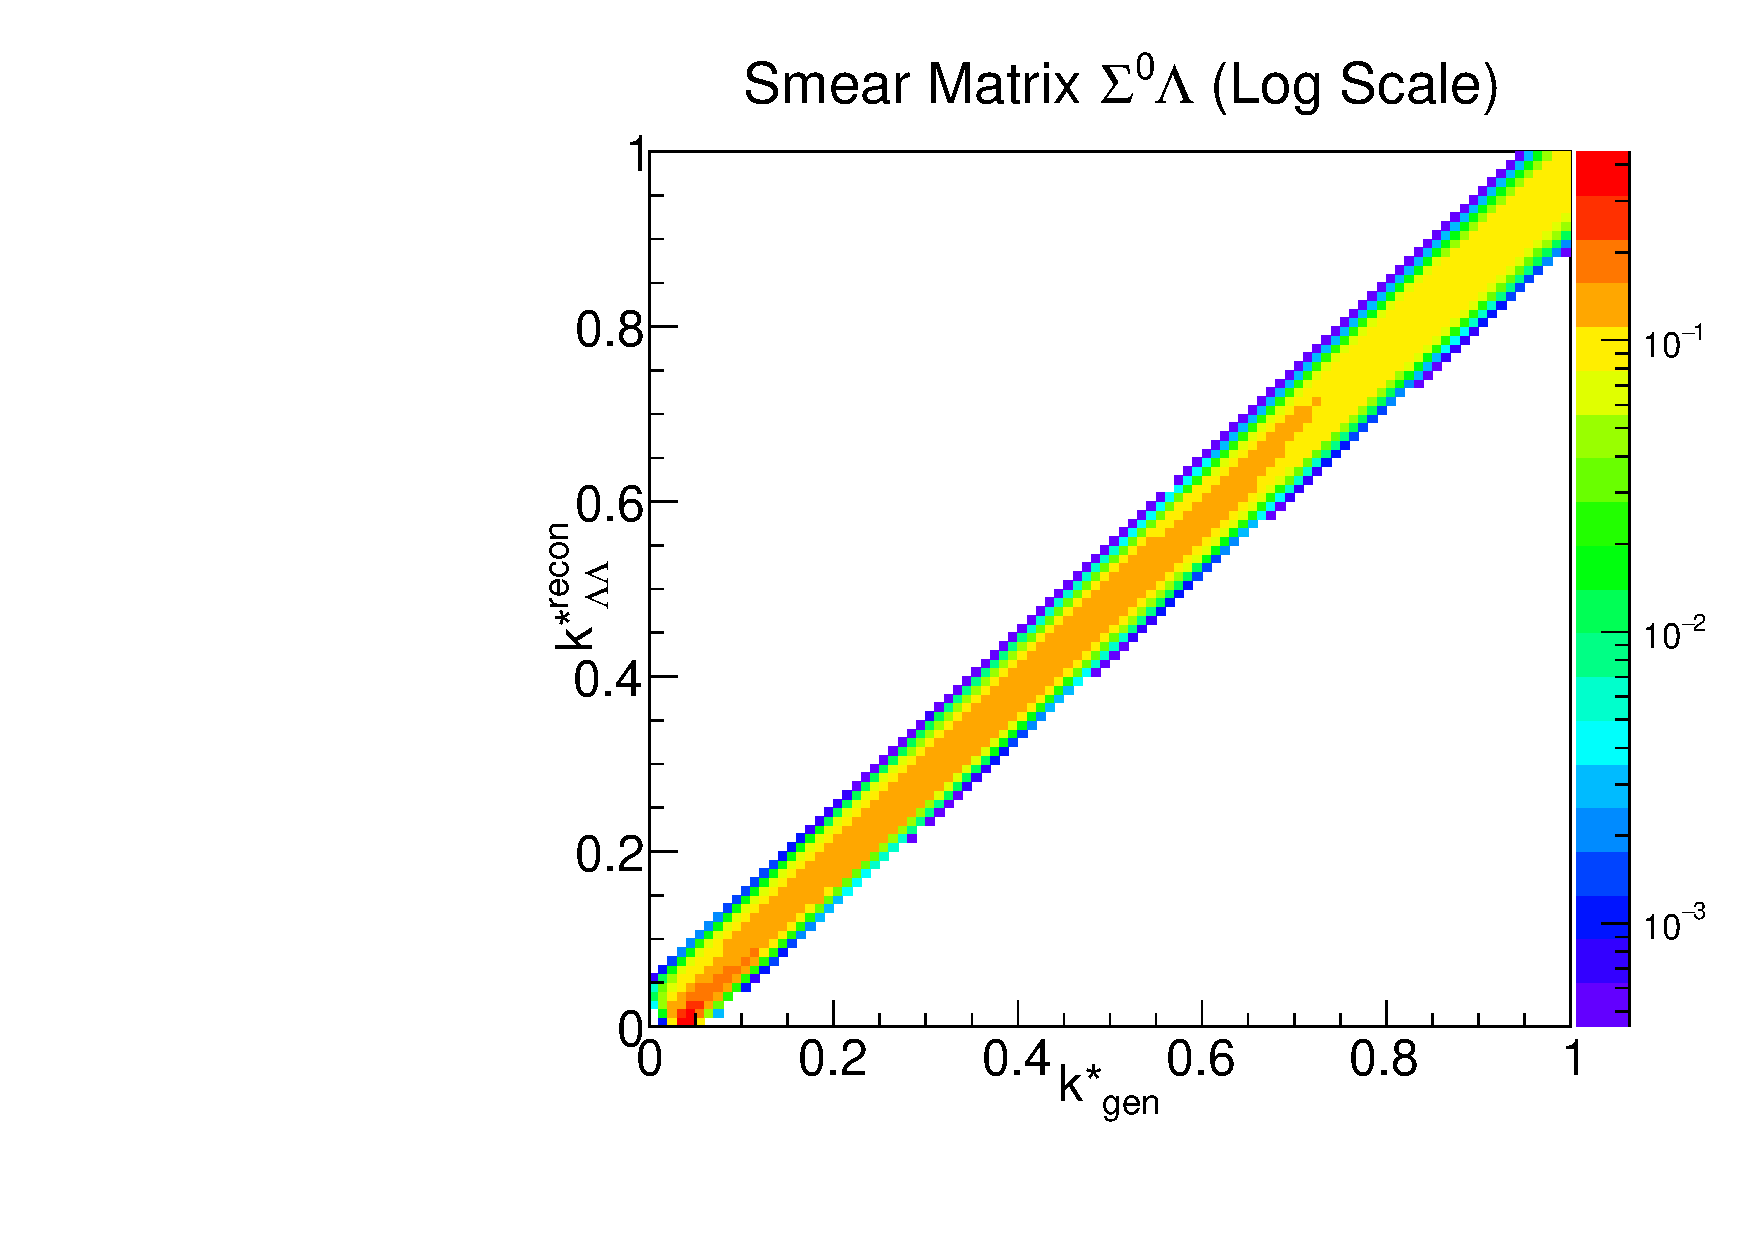
\includegraphics[width=18pc]{Figures/SmearMatrices/2016-7-19-SmearMatrixSigmaLambdaNormLLAALog.pdf}
\end{minipage} 
\caption[Smear matrix -- $\Sigma^0\Lambda$ and $\bar{\Sigma}^0\bar{\Lambda}$]{ 
Smear matrix for $\Sigma^0\Lambda$ and $\bar{\Sigma}^0\bar{\Lambda}$, which accounts for both residual correlation and momentum resolution smearing. This matrix can be used to correct the theoretical correlation function so that the fit has the same smearing as the data.
}
\end{figure}

\begin{figure}[h]
\begin{minipage}{18pc}
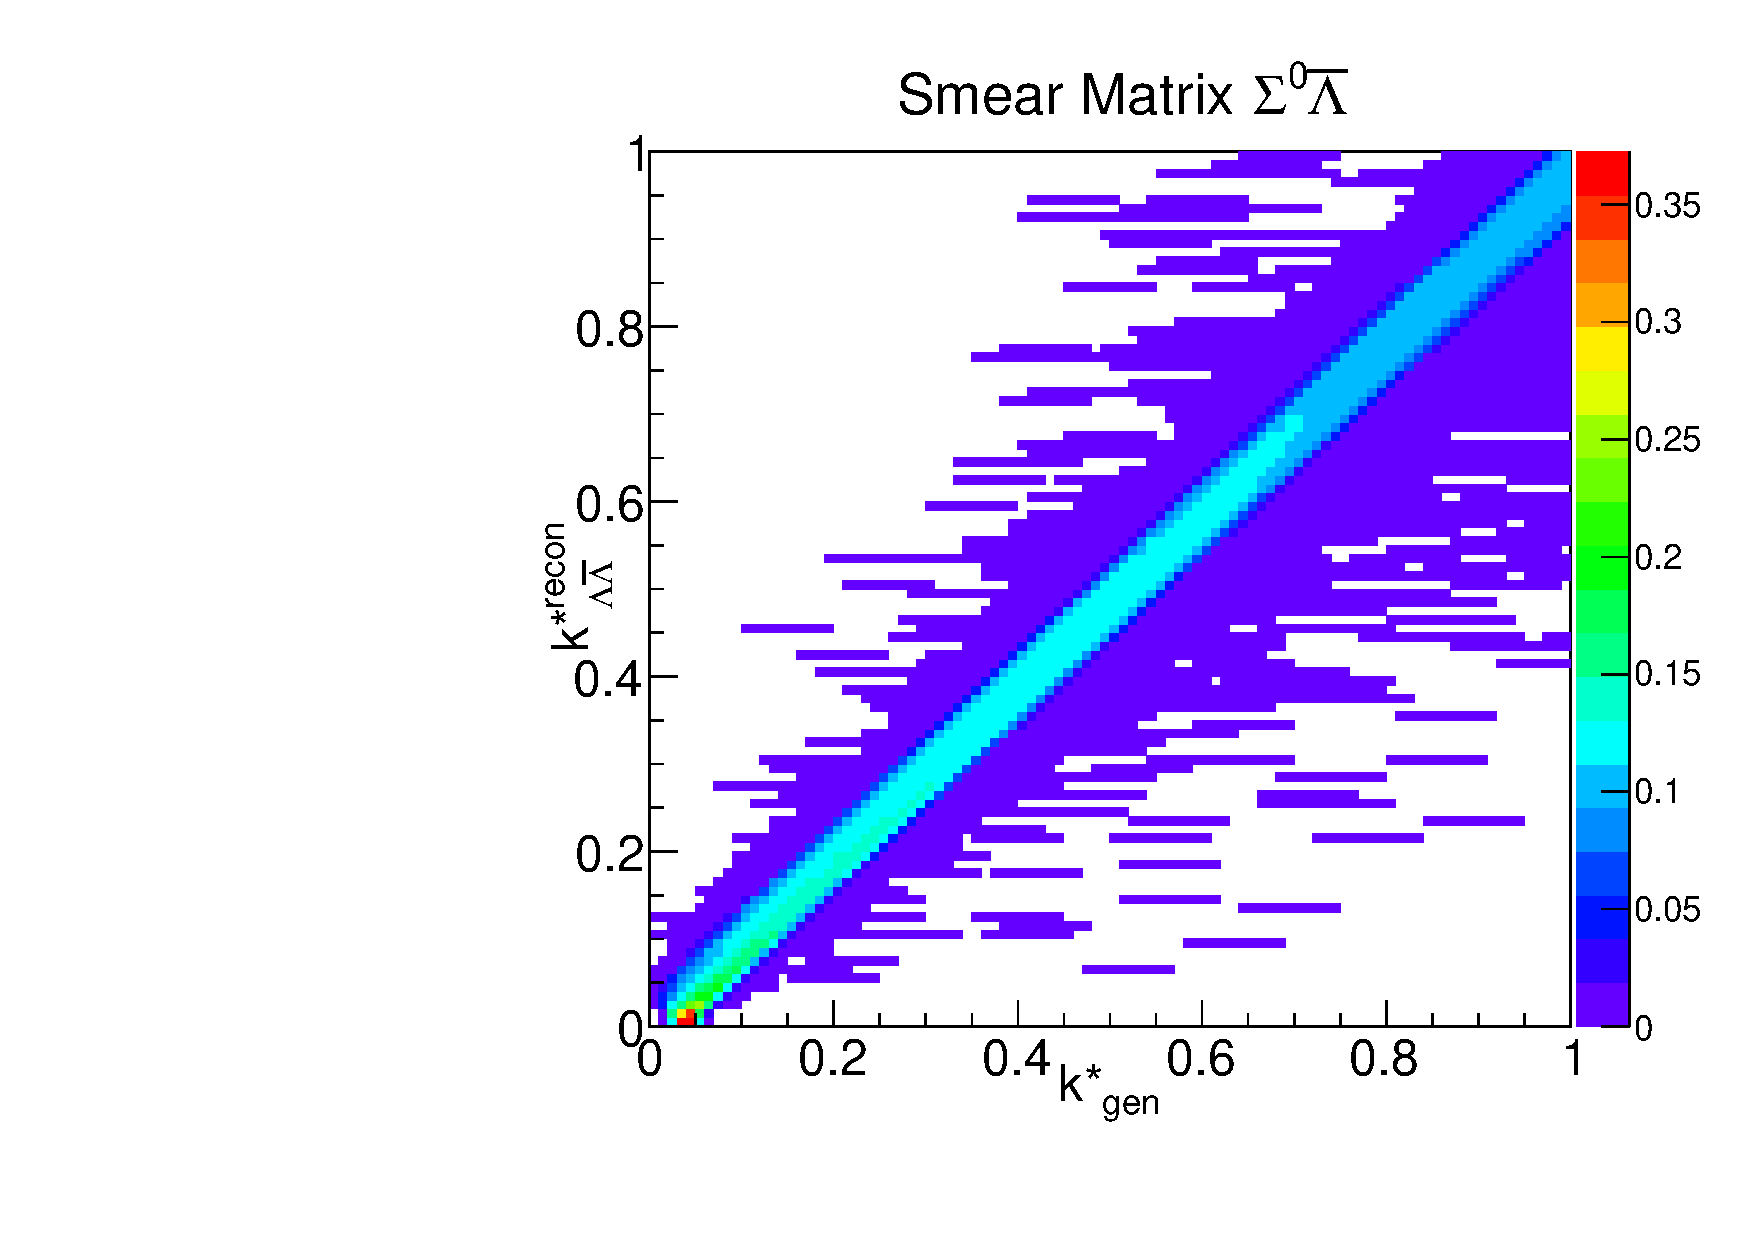
\includegraphics[width=18pc]{Figures/SmearMatrices/2016-7-19-SmearMatrixSigmaLambdaNormLA.pdf}
\end{minipage}\hspace{2pc}
\begin{minipage}{18pc}
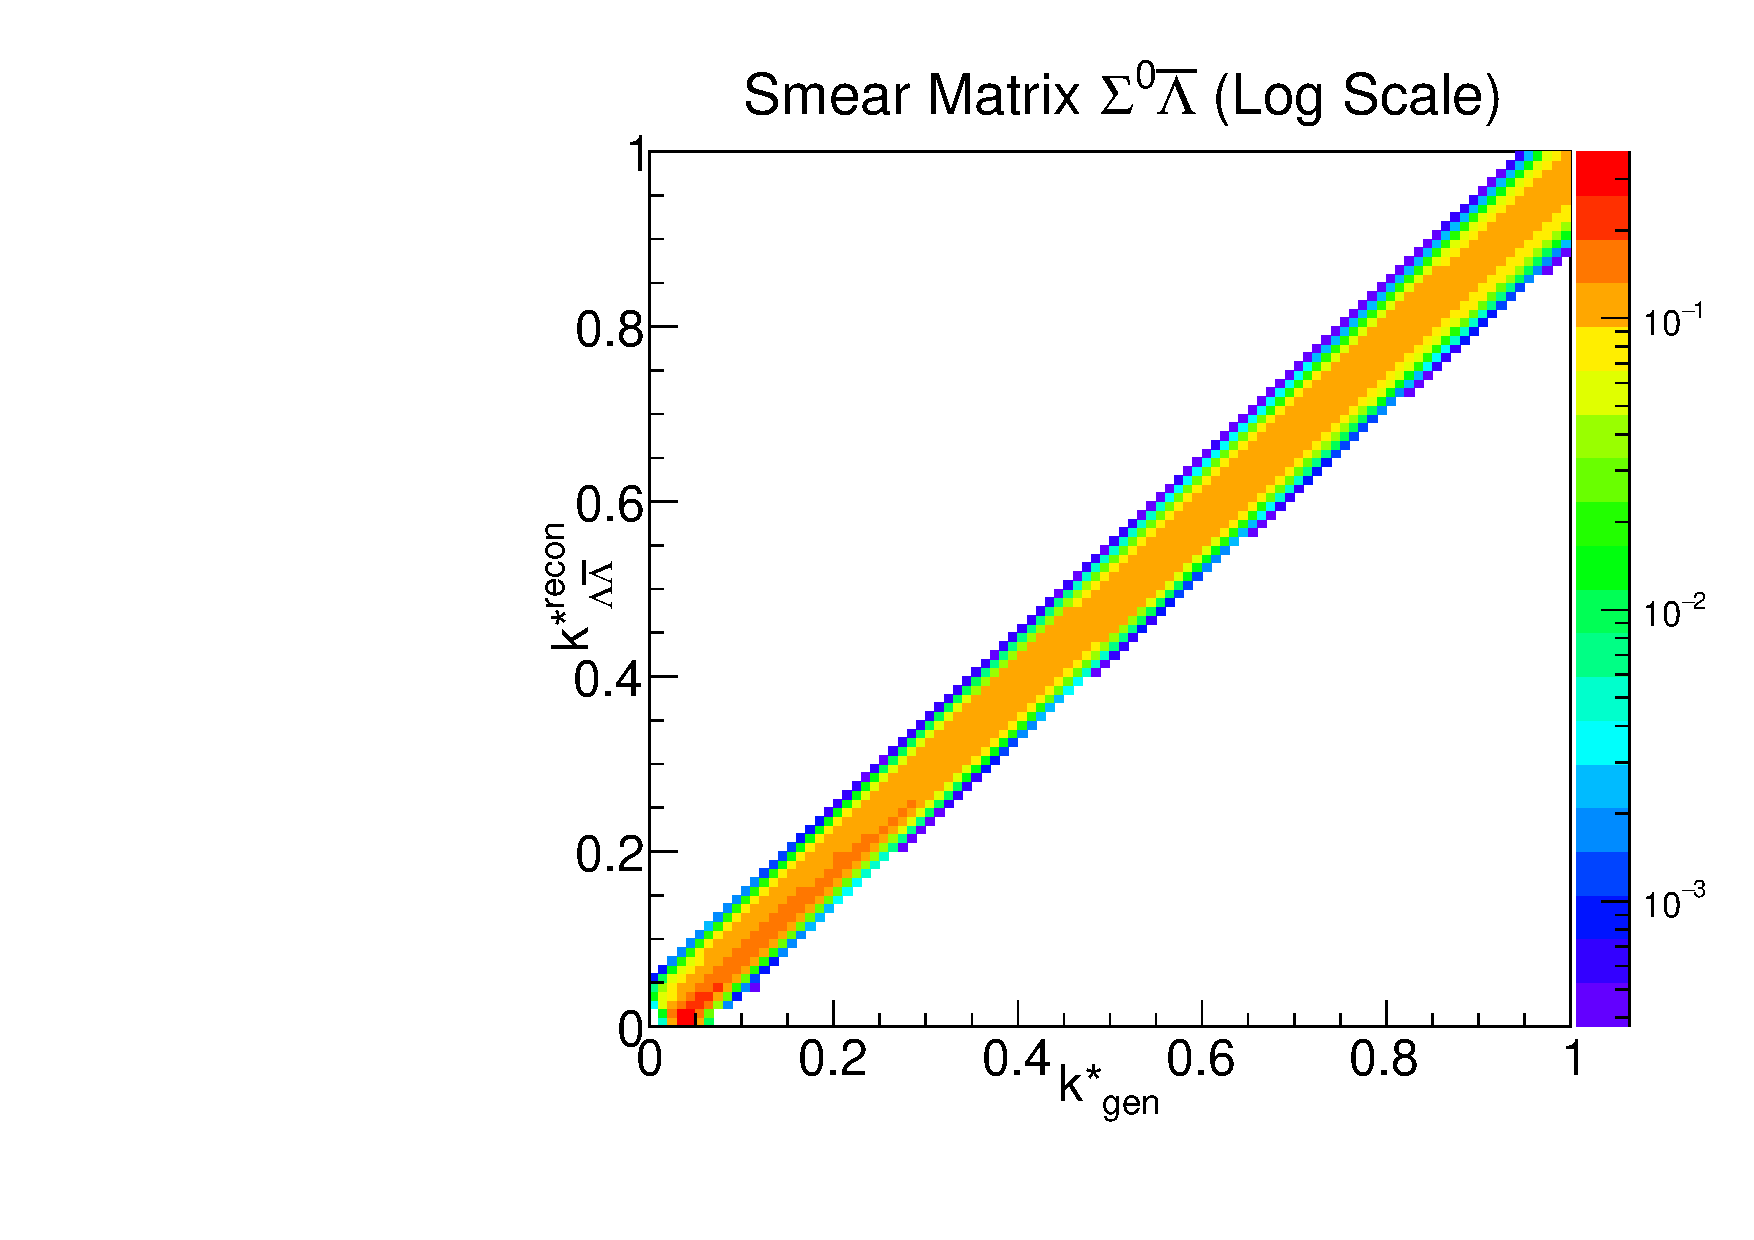
\includegraphics[width=18pc]{Figures/SmearMatrices/2016-7-19-SmearMatrixSigmaLambdaNormLALog.pdf}
\end{minipage} 
\caption[Smear matrix -- $\Sigma^0\bar{\Lambda}$ and $\bar{\Sigma^0}\Lambda$]{
Smear matrix for $\Sigma^0\bar{\Lambda}$ and $\bar{\Sigma^0}\Lambda$, which accounts for both residual correlation and momentum resolution smearing. This matrix can be used to correct the theoretical correlation function so that the fit has the same smearing as the data.
}
\end{figure}


\begin{figure}[h]
\begin{minipage}{18pc}
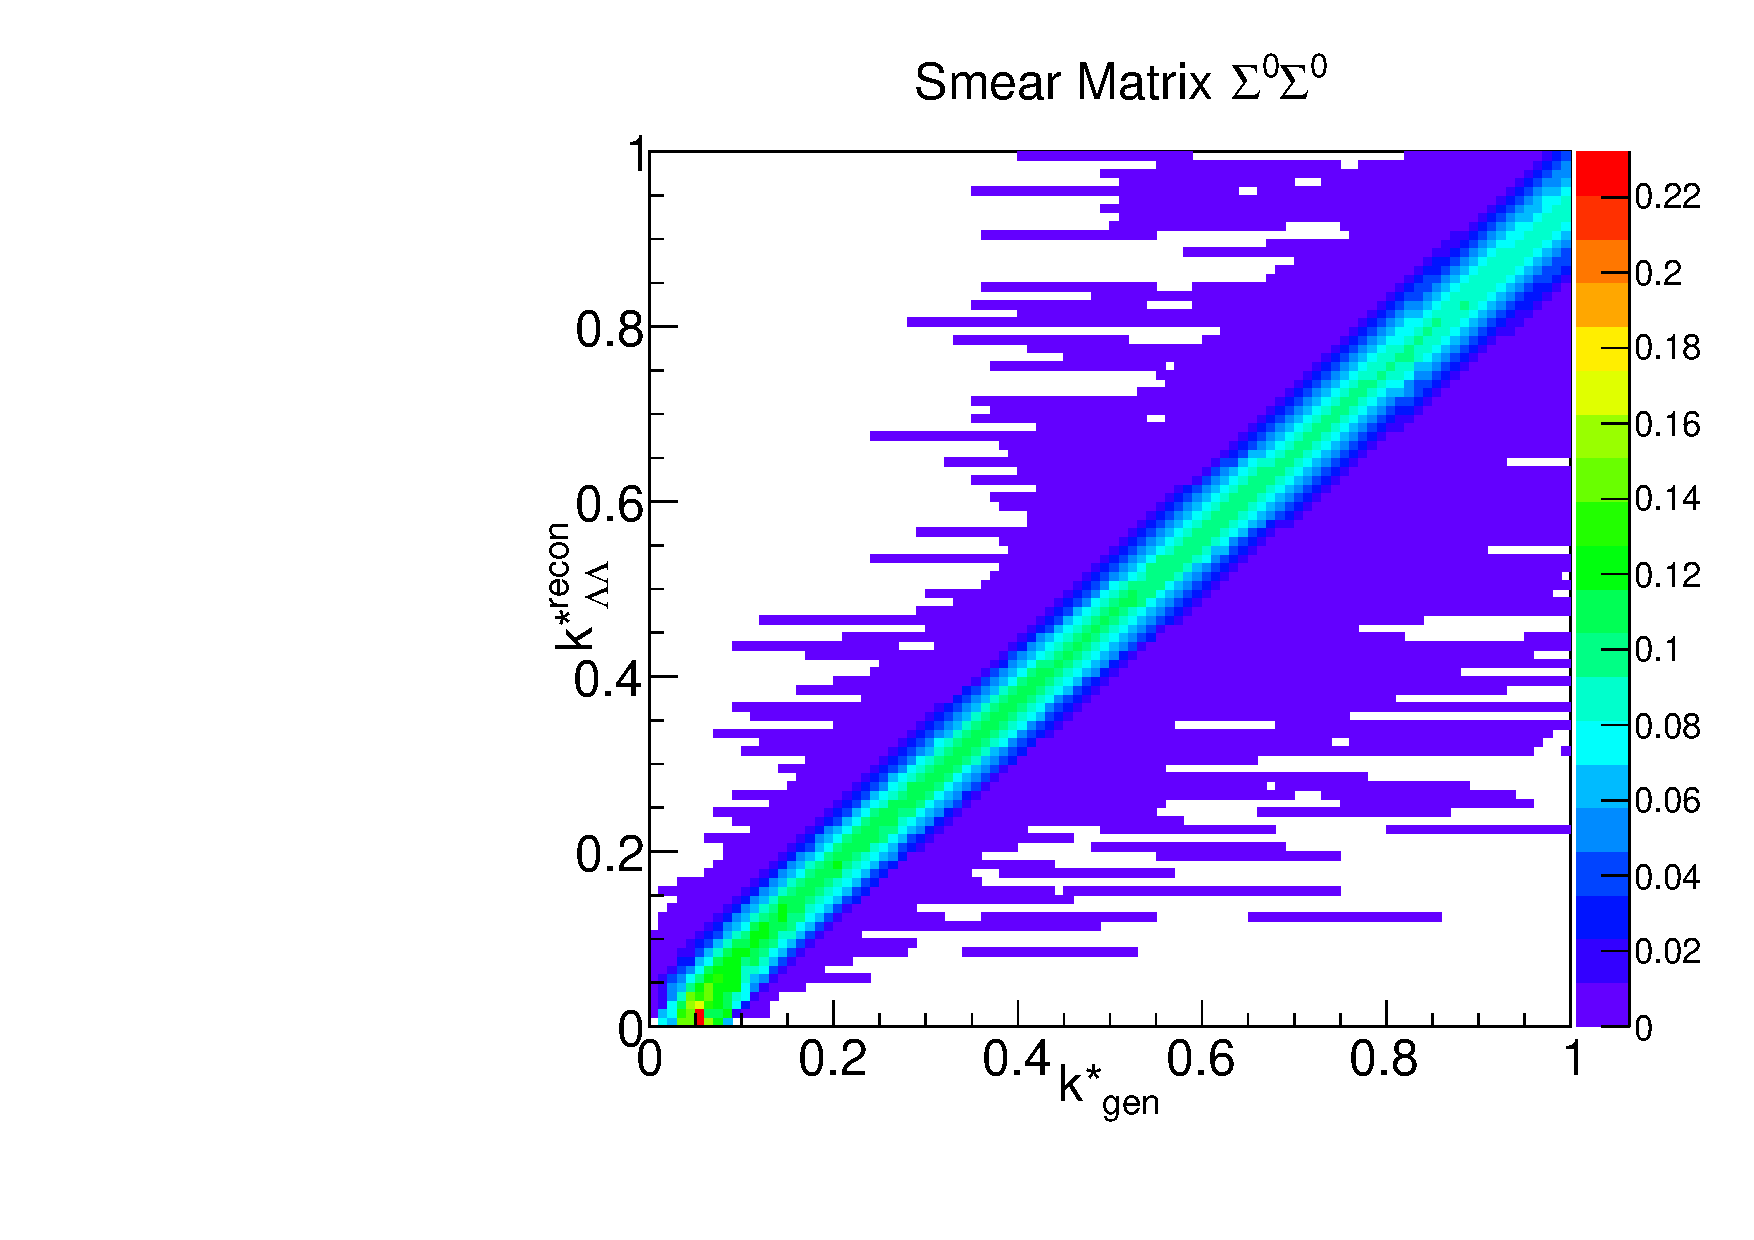
\includegraphics[width=18pc]{Figures/SmearMatrices/2016-7-19-SmearMatrixSigmaSigmaNormLLAA.pdf}
\end{minipage}\hspace{2pc}
\begin{minipage}{18pc}
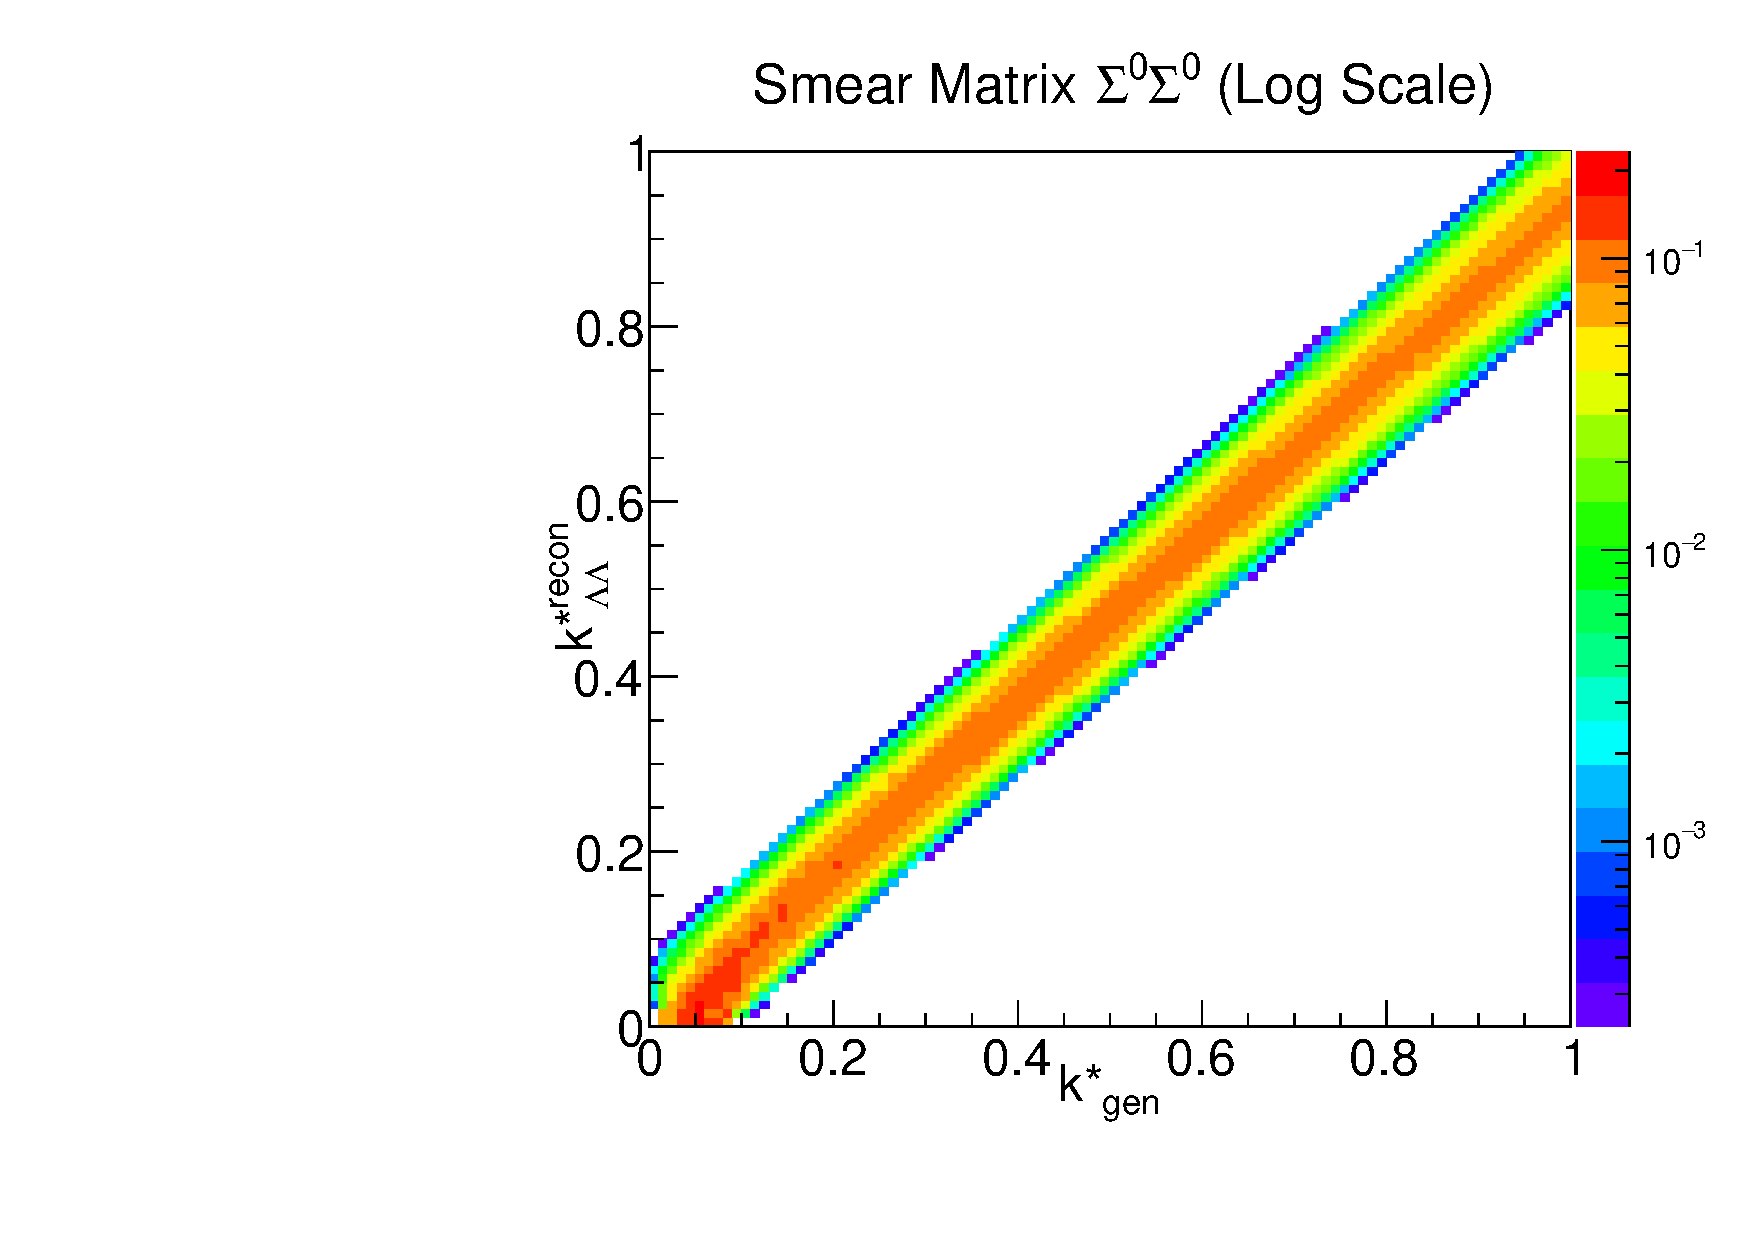
\includegraphics[width=18pc]{Figures/SmearMatrices/2016-7-19-SmearMatrixSigmaSigmaNormLLAALog.pdf}
\end{minipage} 
\caption[Smear matrix -- $\Sigma^0\Sigma^0$ and $\bar{\Sigma}^0\bar{\Sigma}^0$]{
Smear matrix for $\Sigma^0\Sigma^0$ and $\bar{\Sigma}^0\bar{\Sigma}^0$, which accounts for both residual correlation and momentum resolution smearing. This matrix can be used to correct the theoretical correlation function so that the fit has the same smearing as the data.
}
\end{figure}


\begin{figure}[h]
\begin{minipage}{18pc}
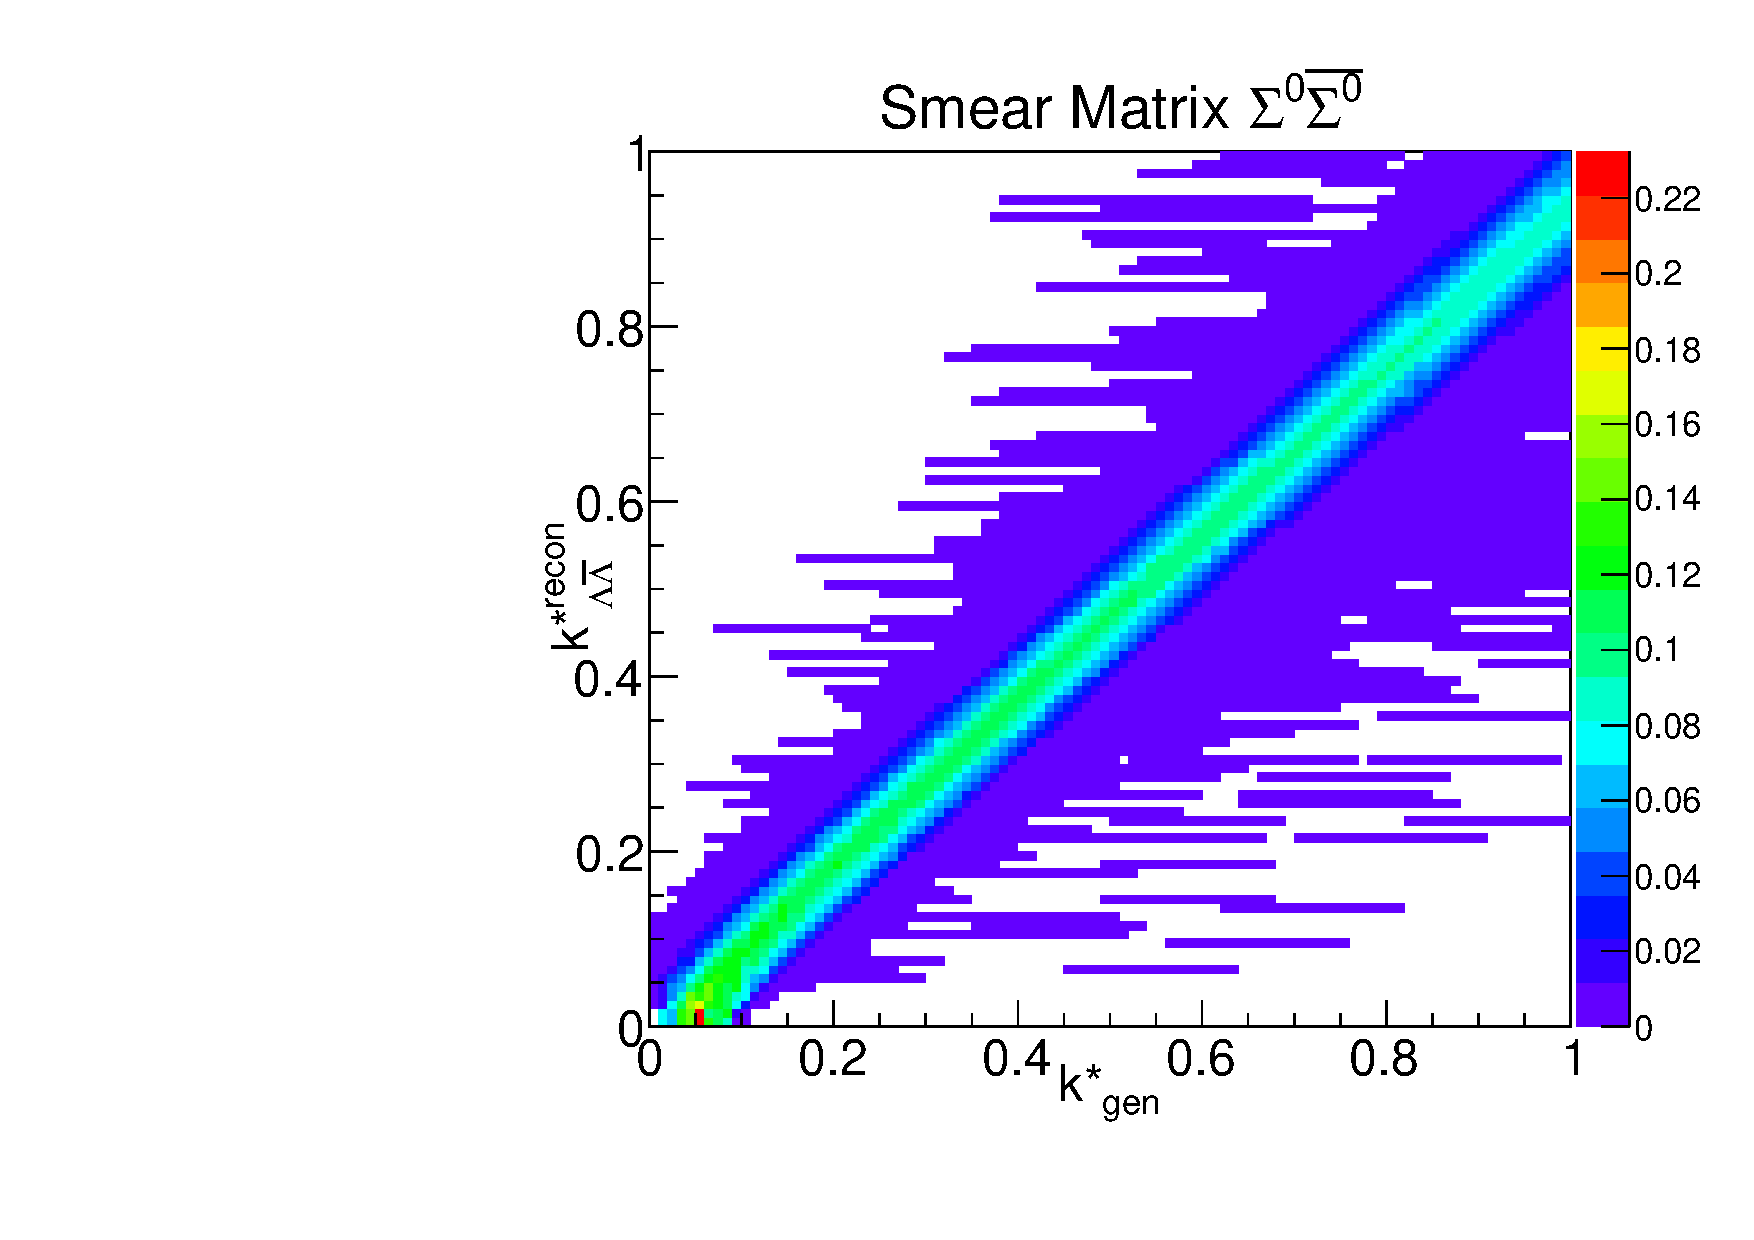
\includegraphics[width=18pc]{Figures/SmearMatrices/2016-7-19-SmearMatrixSigmaSigmaNormLA.pdf}
\end{minipage}\hspace{2pc}
\begin{minipage}{18pc}
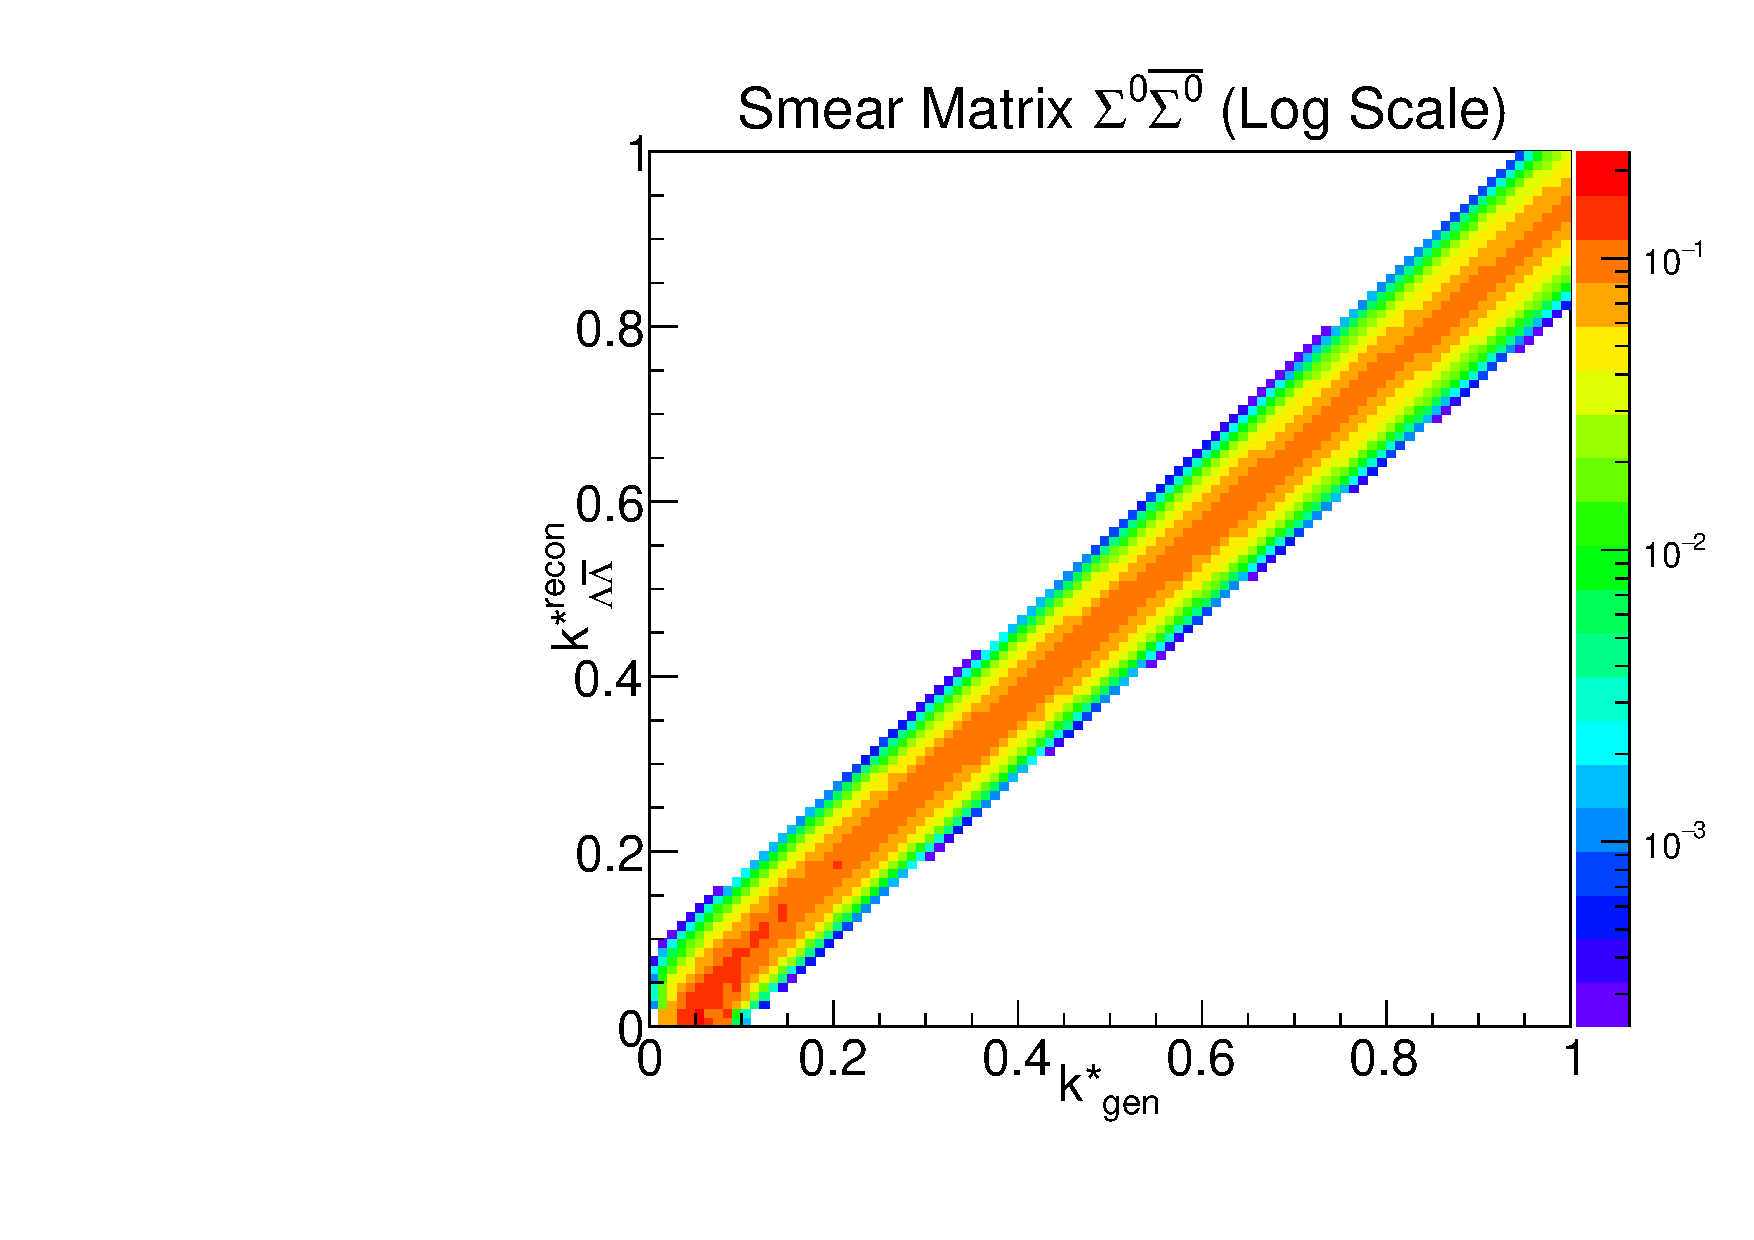
\includegraphics[width=18pc]{Figures/SmearMatrices/2016-7-19-SmearMatrixSigmaSigmaNormLALog.pdf}
\end{minipage} 
\caption[Smear matrix -- $\Sigma^0\bar{\Sigma}^0$]{
Smear matrix for $\Sigma^0\bar{\Sigma}^0$, which accounts for both residual correlation and momentum resolution smearing. This matrix can be used to correct the theoretical correlation function so that the fit has the same smearing as the data.
}
\end{figure}


\begin{figure}[h]
\begin{minipage}{18pc}
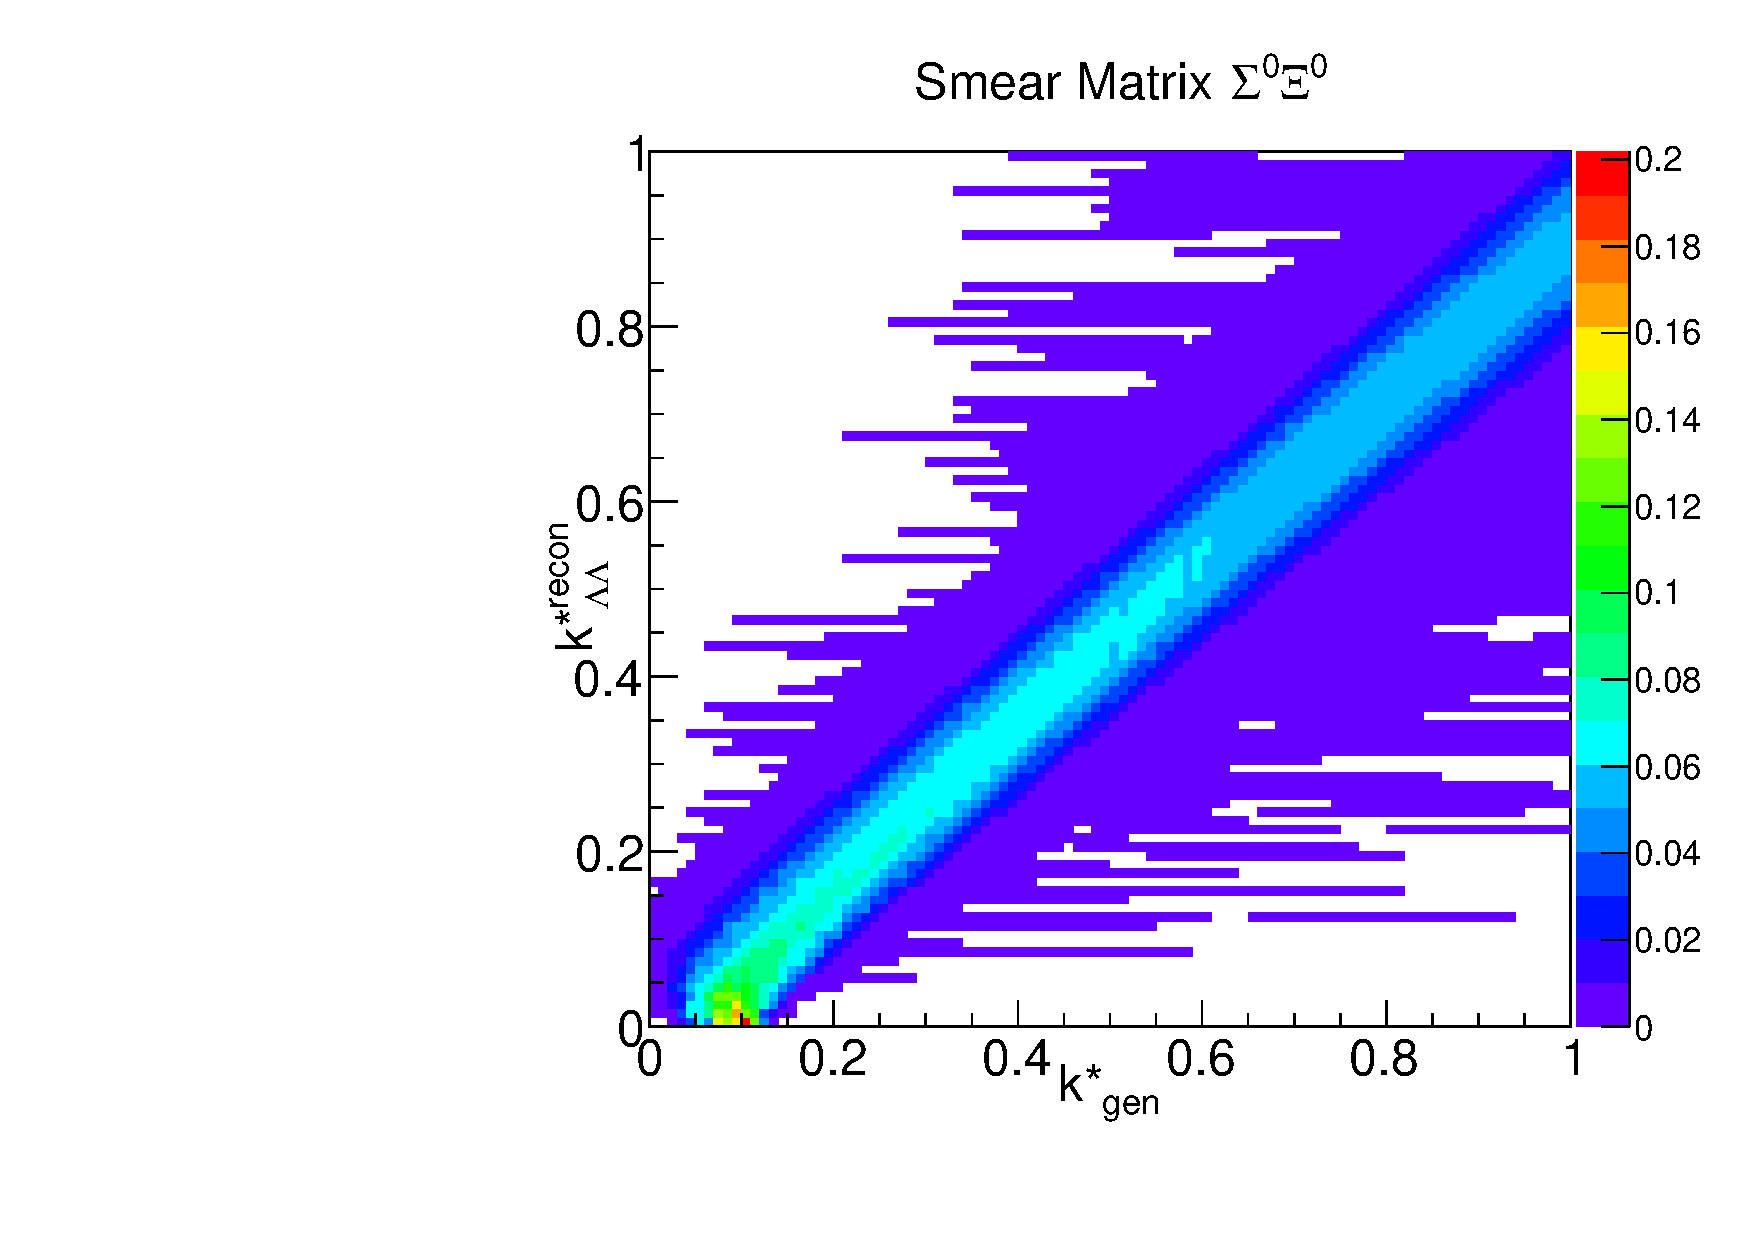
\includegraphics[width=18pc]{Figures/SmearMatrices/2016-7-19-SmearMatrixSigmaXi0NormLLAA.pdf}
\end{minipage}\hspace{2pc}
\begin{minipage}{18pc}
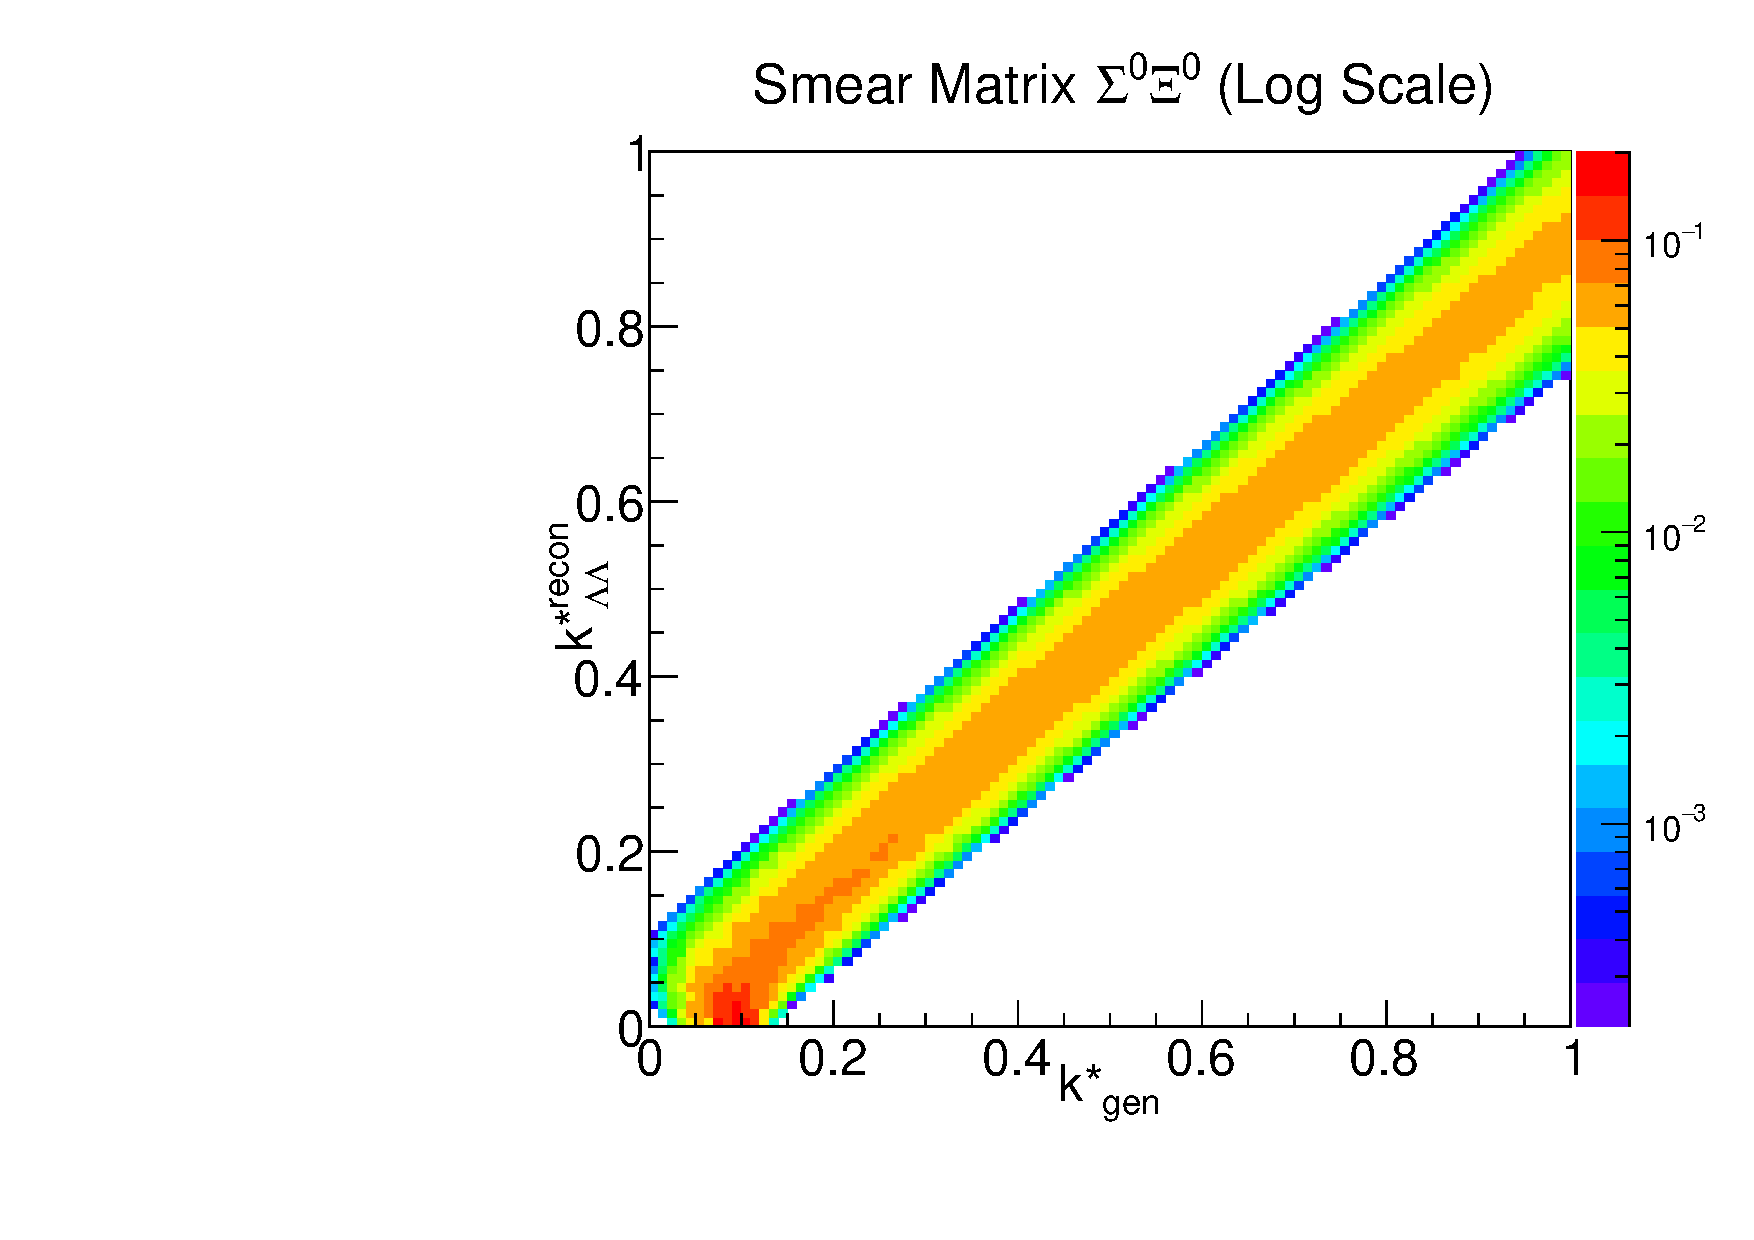
\includegraphics[width=18pc]{Figures/SmearMatrices/2016-7-19-SmearMatrixSigmaXi0NormLLAALog.pdf}
\end{minipage} 
\caption[Smear matrix -- $\Sigma^0\Xi^0$ and $\bar{\Sigma}^0\bar{\Xi}^0$]{
Smear matrix for $\Sigma^0\Xi^0$ and $\bar{\Sigma}^0\bar{\Xi}^0$, which accounts for both residual correlation and momentum resolution smearing. This matrix can be used to correct the theoretical correlation function so that the fit has the same smearing as the data.
}
\end{figure}


\begin{figure}[h]
\begin{minipage}{18pc}
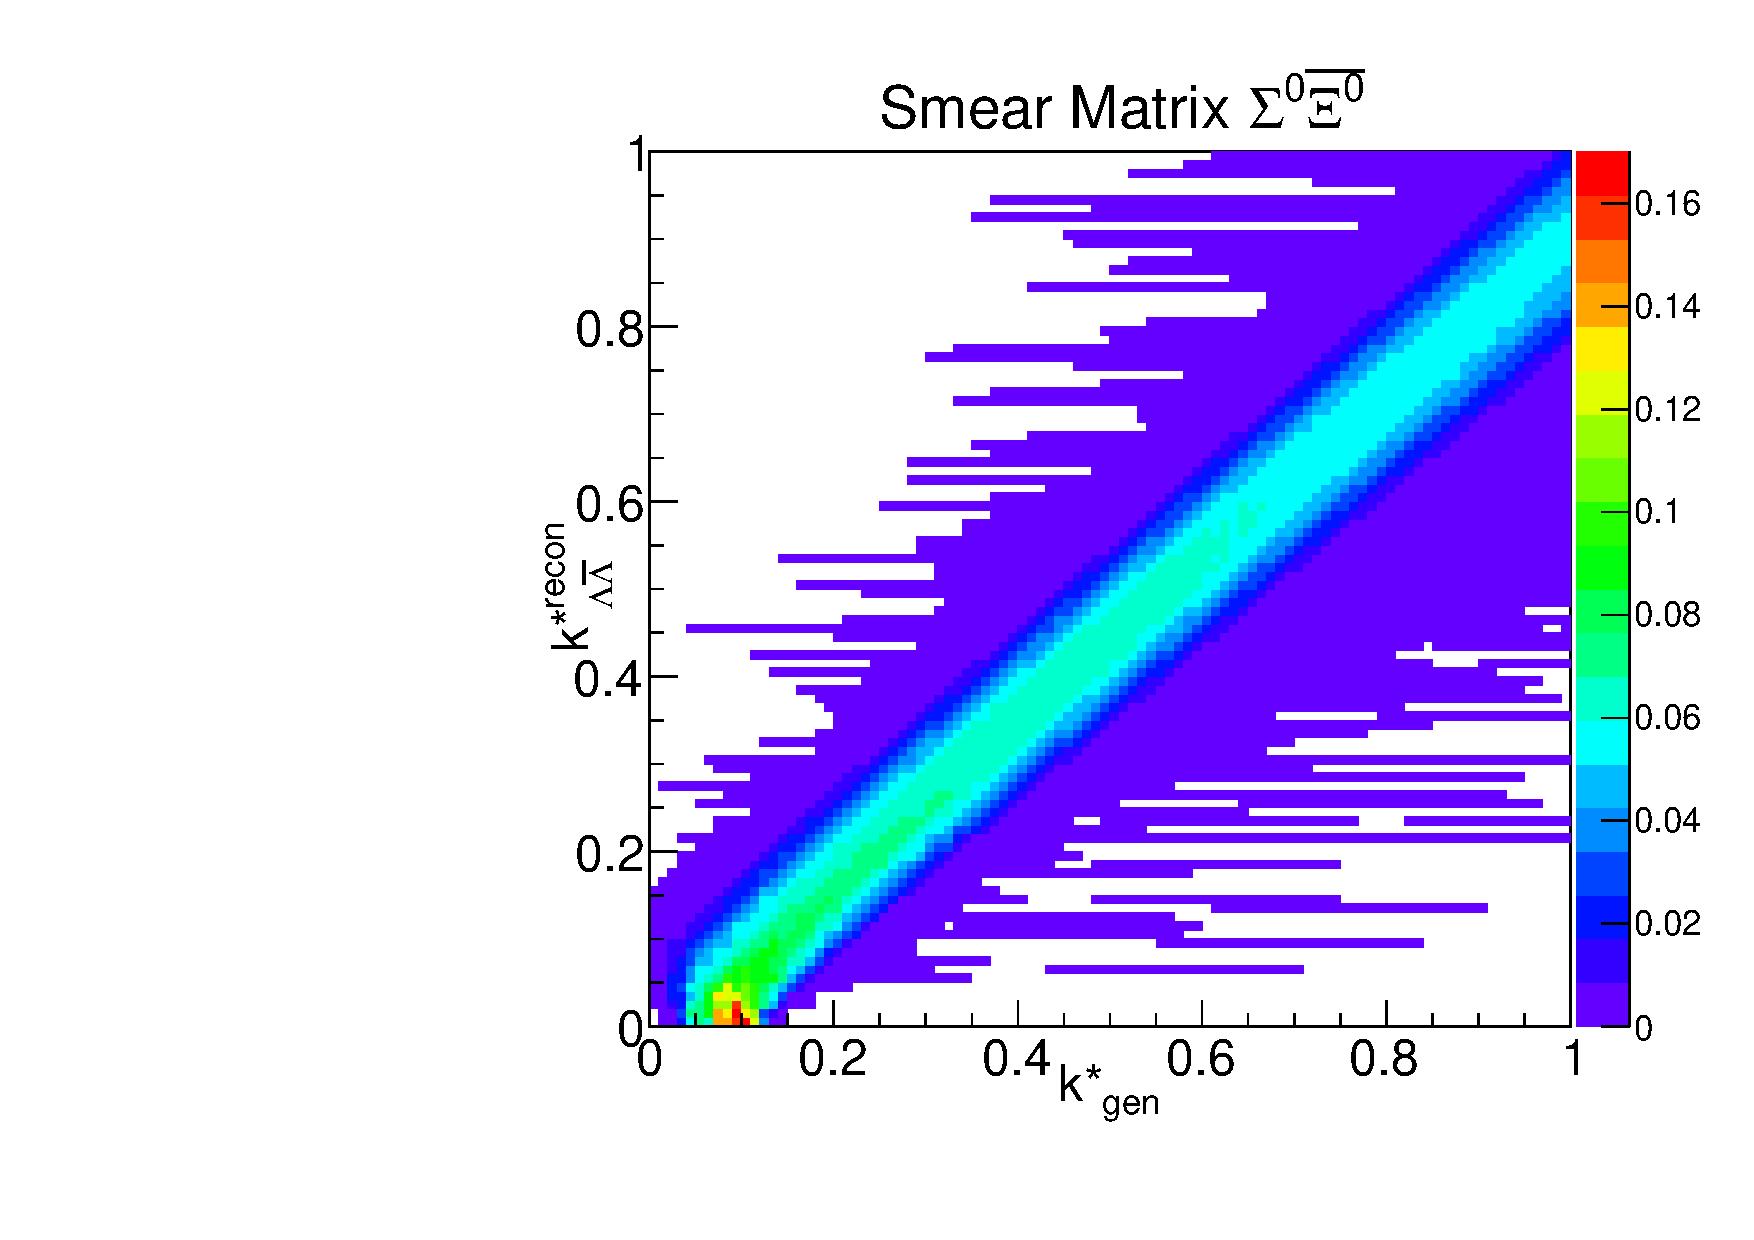
\includegraphics[width=18pc]{Figures/SmearMatrices/2016-7-19-SmearMatrixSigmaXi0NormLA.pdf}
\end{minipage}\hspace{2pc}
\begin{minipage}{18pc}
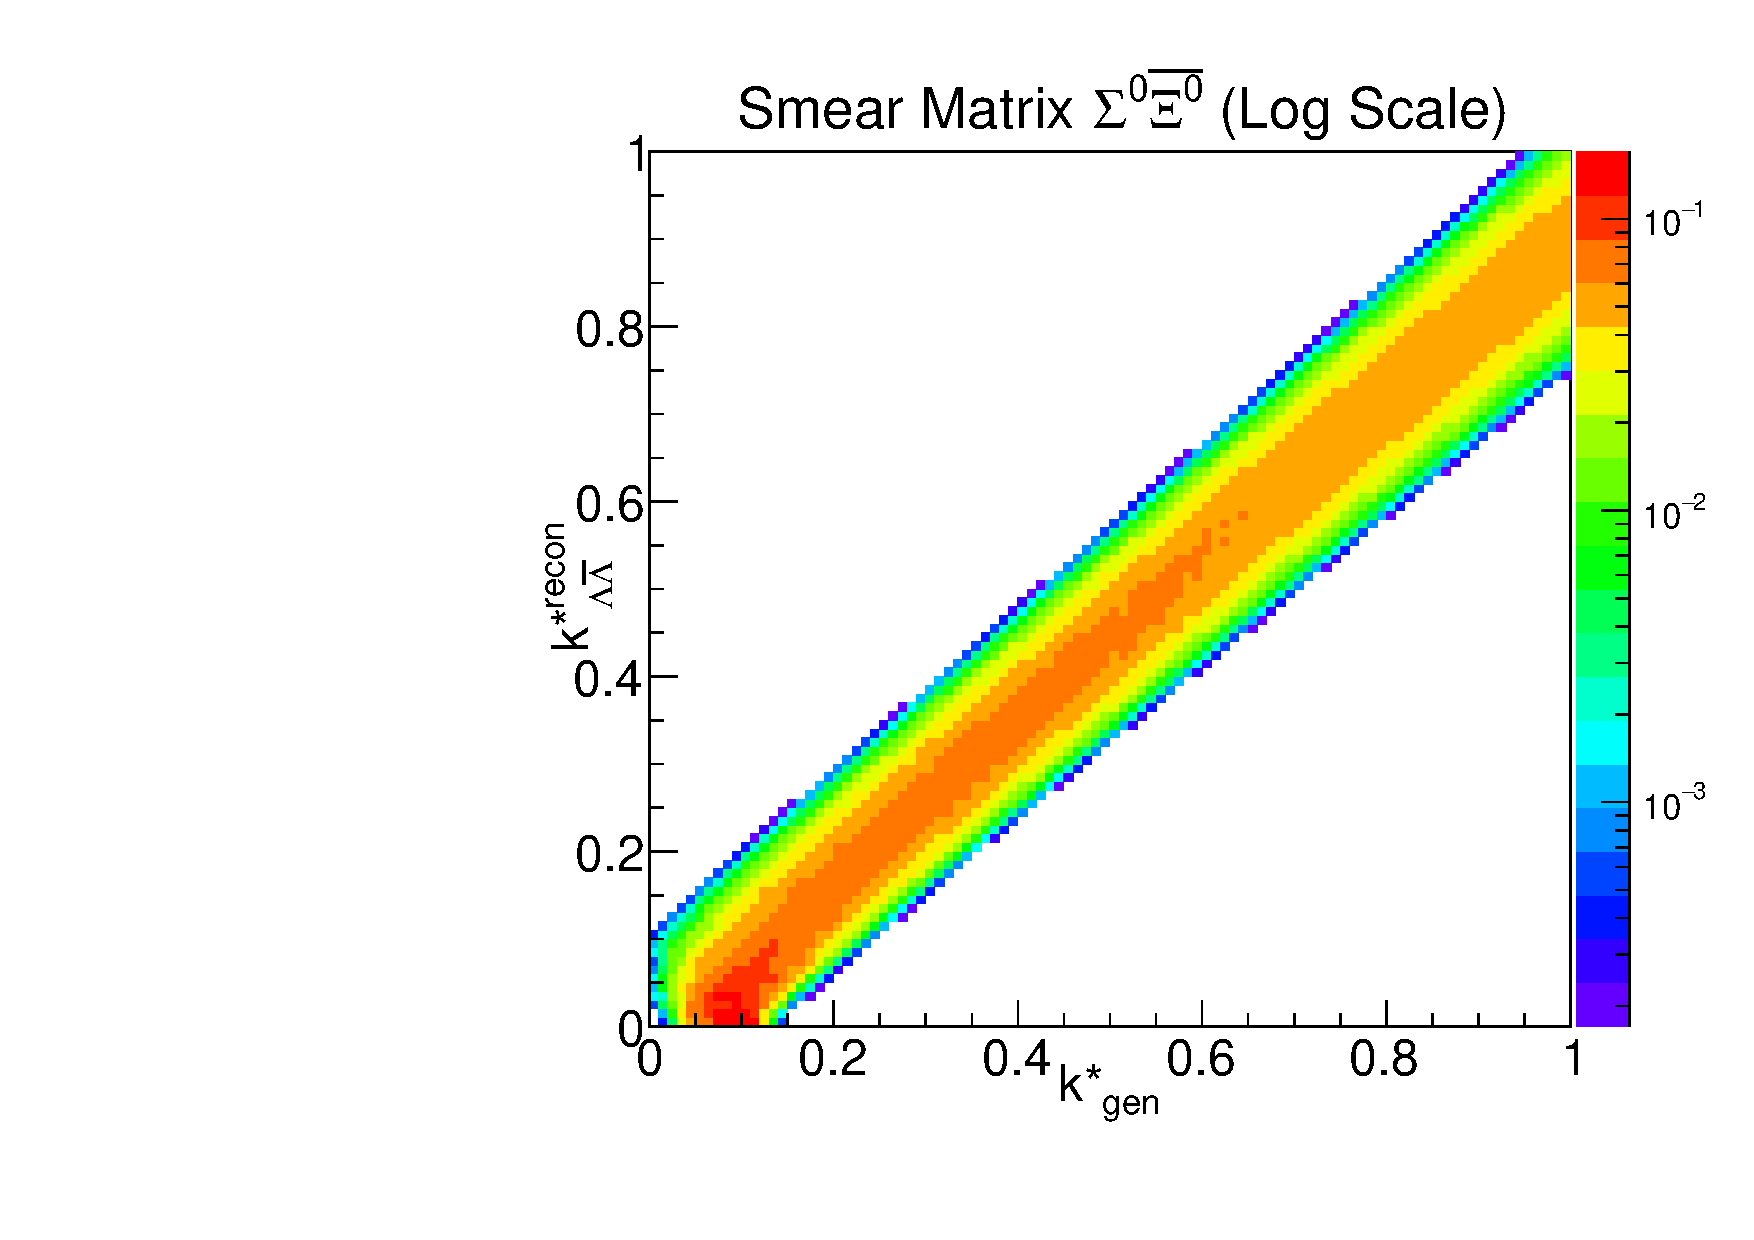
\includegraphics[width=18pc]{Figures/SmearMatrices/2016-7-19-SmearMatrixSigmaXi0NormLALog.pdf}
\end{minipage} 
\caption[Smear matrix -- $\Sigma^0\bar{\Xi}^0$ and $\bar{\Sigma}^0\Xi^0$]{
Smear matrix for $\Sigma^0\bar{\Xi}^0$ and $\bar{\Sigma}^0\Xi^0$, which accounts for both residual correlation and momentum resolution smearing. This matrix can be used to correct the theoretical correlation function so that the fit has the same smearing as the data.
}
\end{figure}


\begin{figure}[h]
\begin{minipage}{18pc}
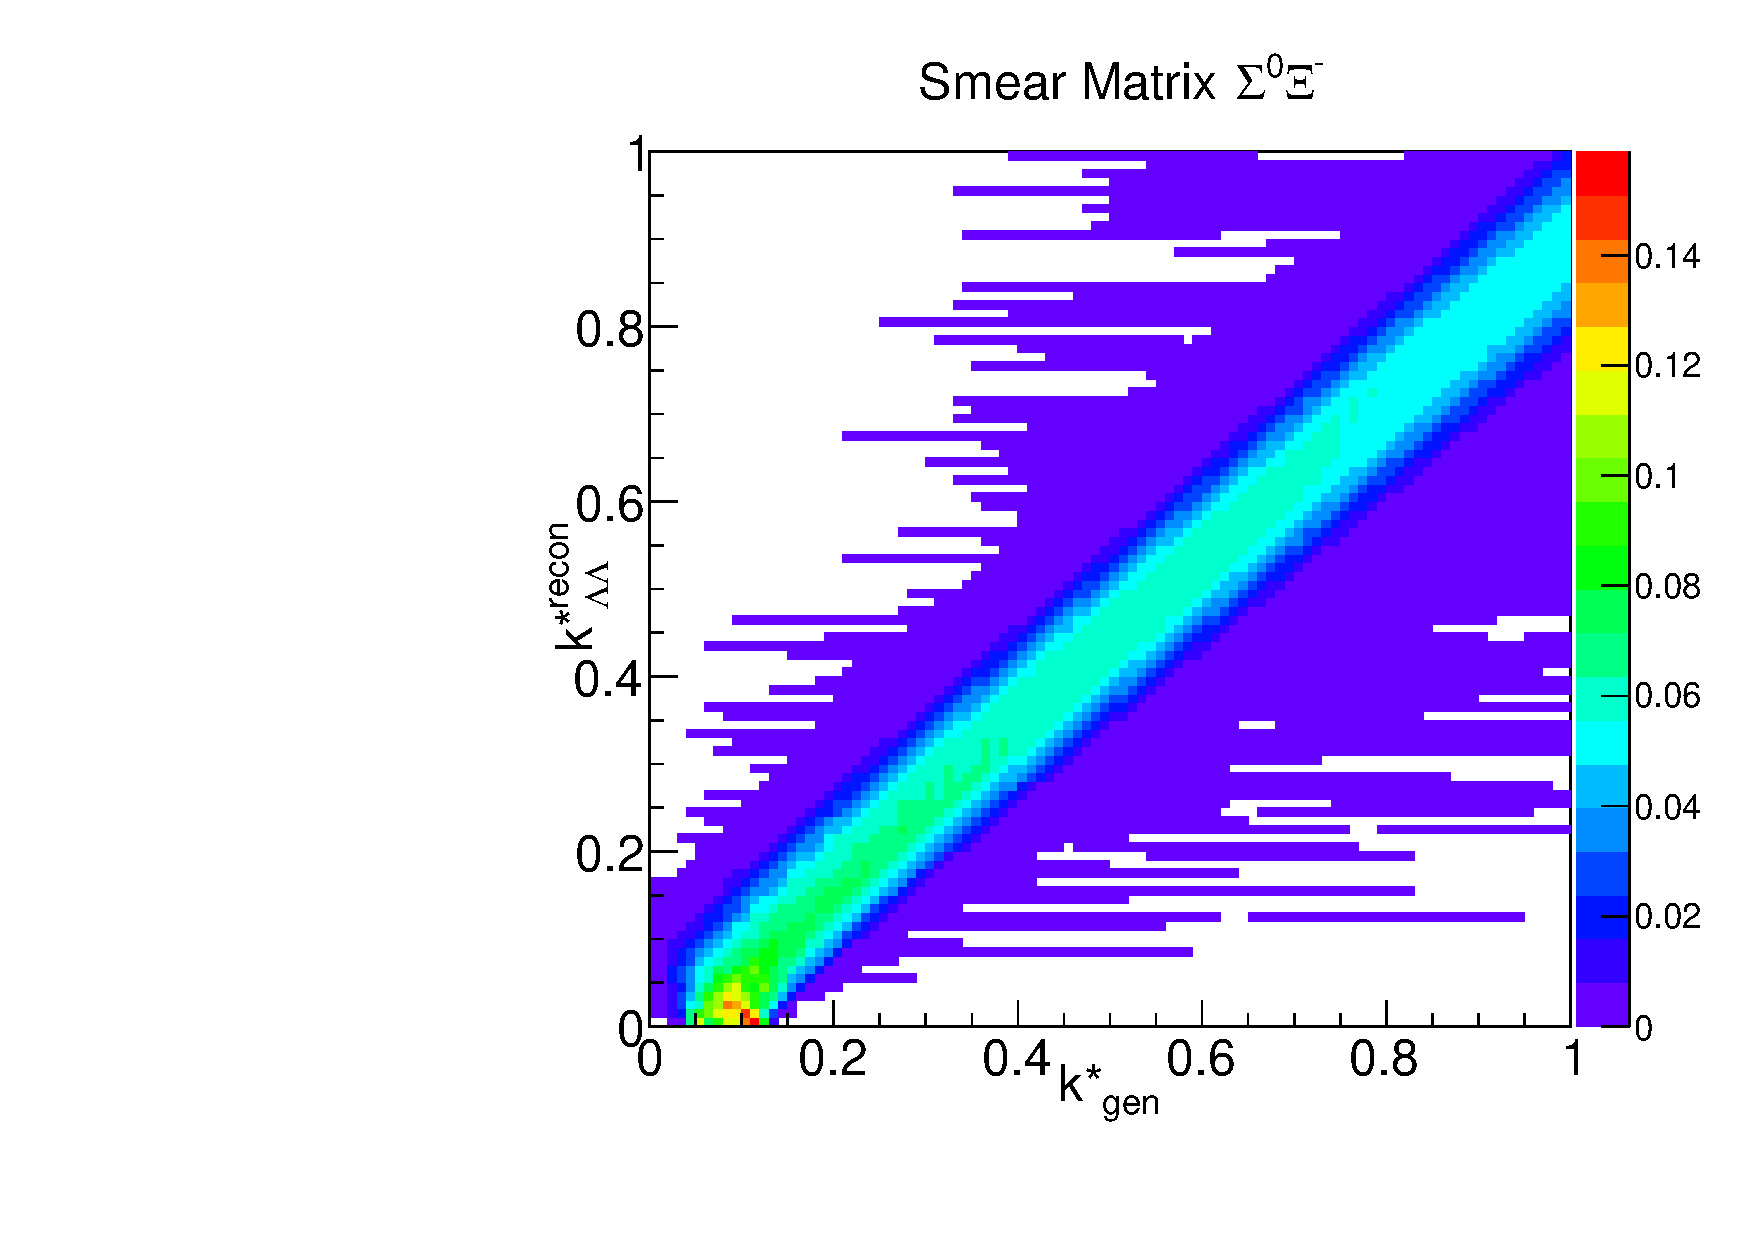
\includegraphics[width=18pc]{Figures/SmearMatrices/2016-7-19-SmearMatrixSigmaXiCNormLLAA.pdf}
\end{minipage}\hspace{2pc}
\begin{minipage}{18pc}
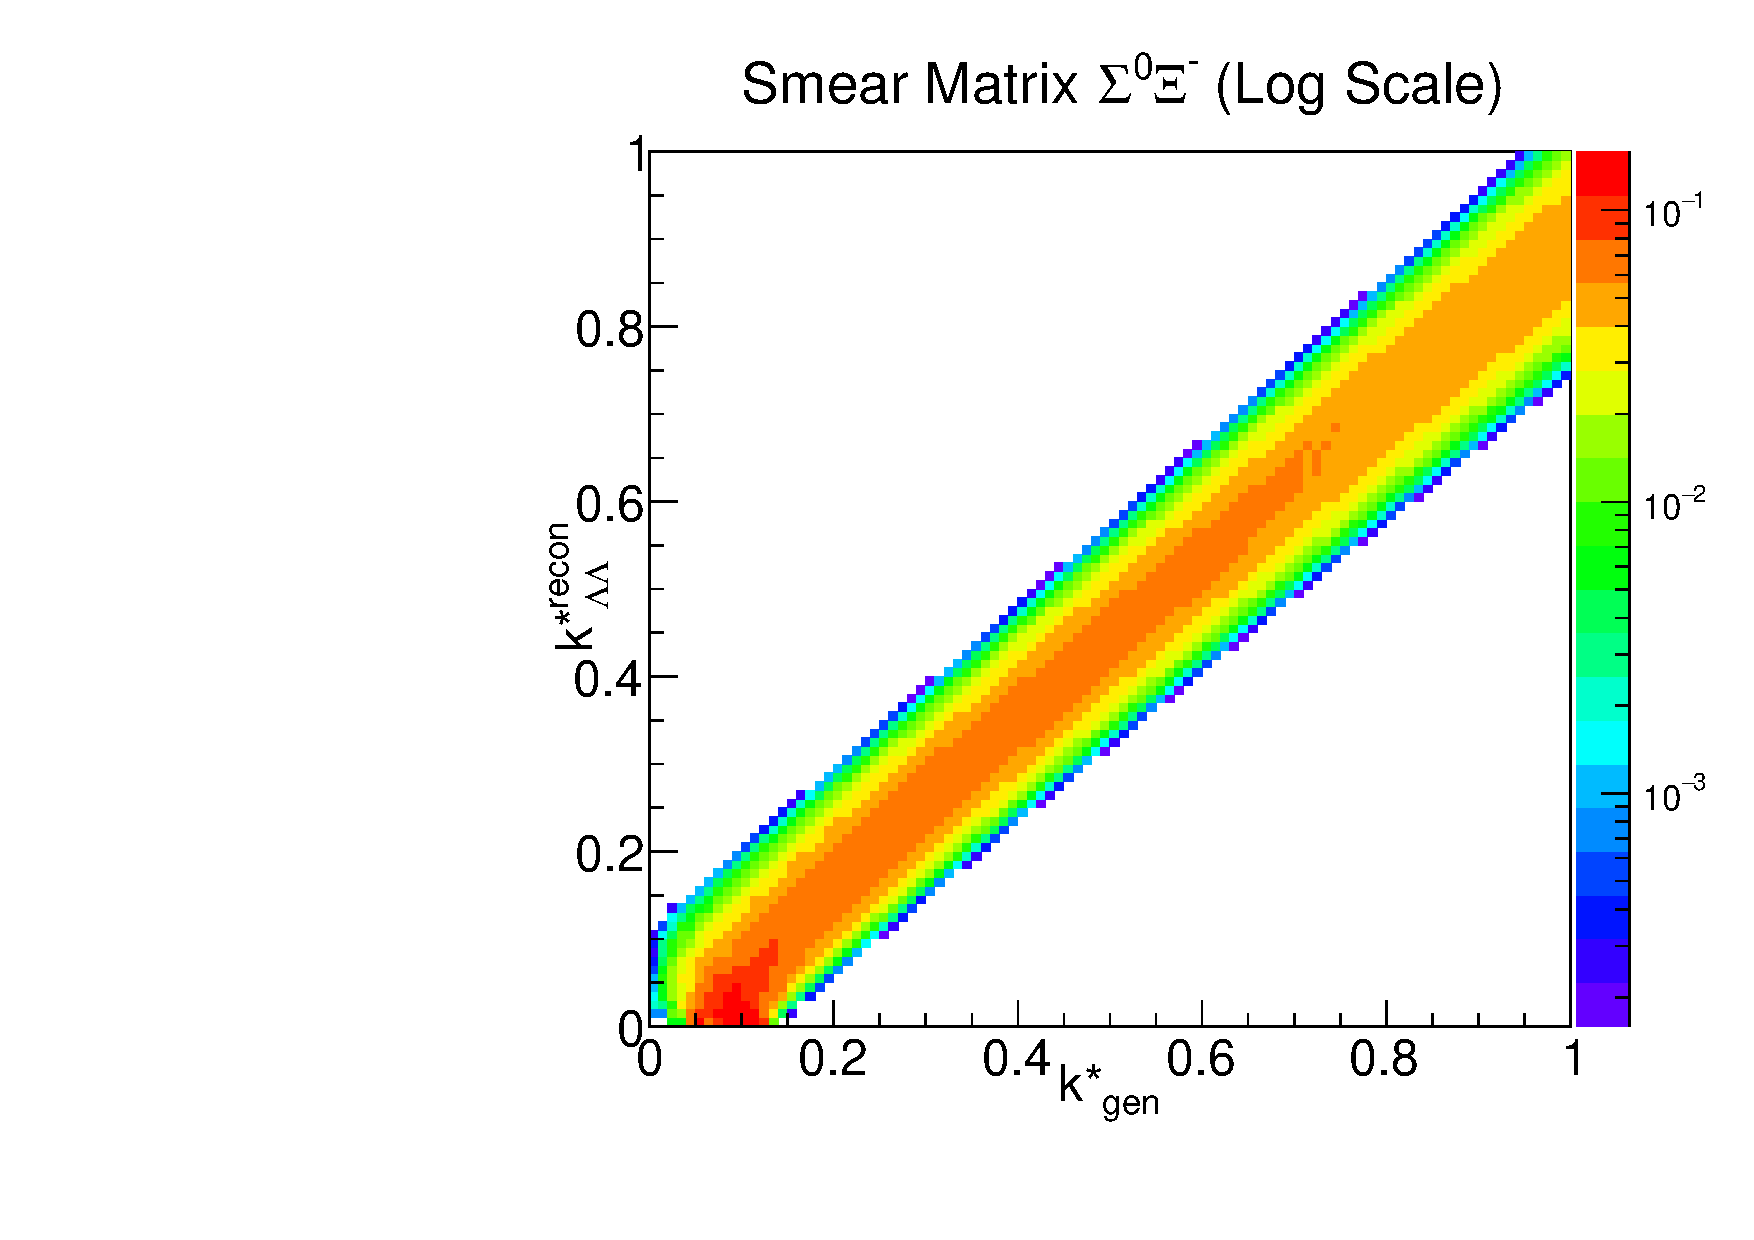
\includegraphics[width=18pc]{Figures/SmearMatrices/2016-7-19-SmearMatrixSigmaXiCNormLLAALog.pdf}
\end{minipage} 
\caption[Smear matrix -- $\Sigma^0\Xi^{-}$ and $\bar{\Sigma}^0\Xi^{+}$]{
Smear matrix for $\Sigma^0\Xi^{-}$ and $\bar{\Sigma}^0\Xi^{+}$, which accounts for both residual correlation and momentum resolution smearing. This matrix can be used to correct the theoretical correlation function so that the fit has the same smearing as the data.
}
\end{figure}


\begin{figure}[h]
\begin{minipage}{18pc}
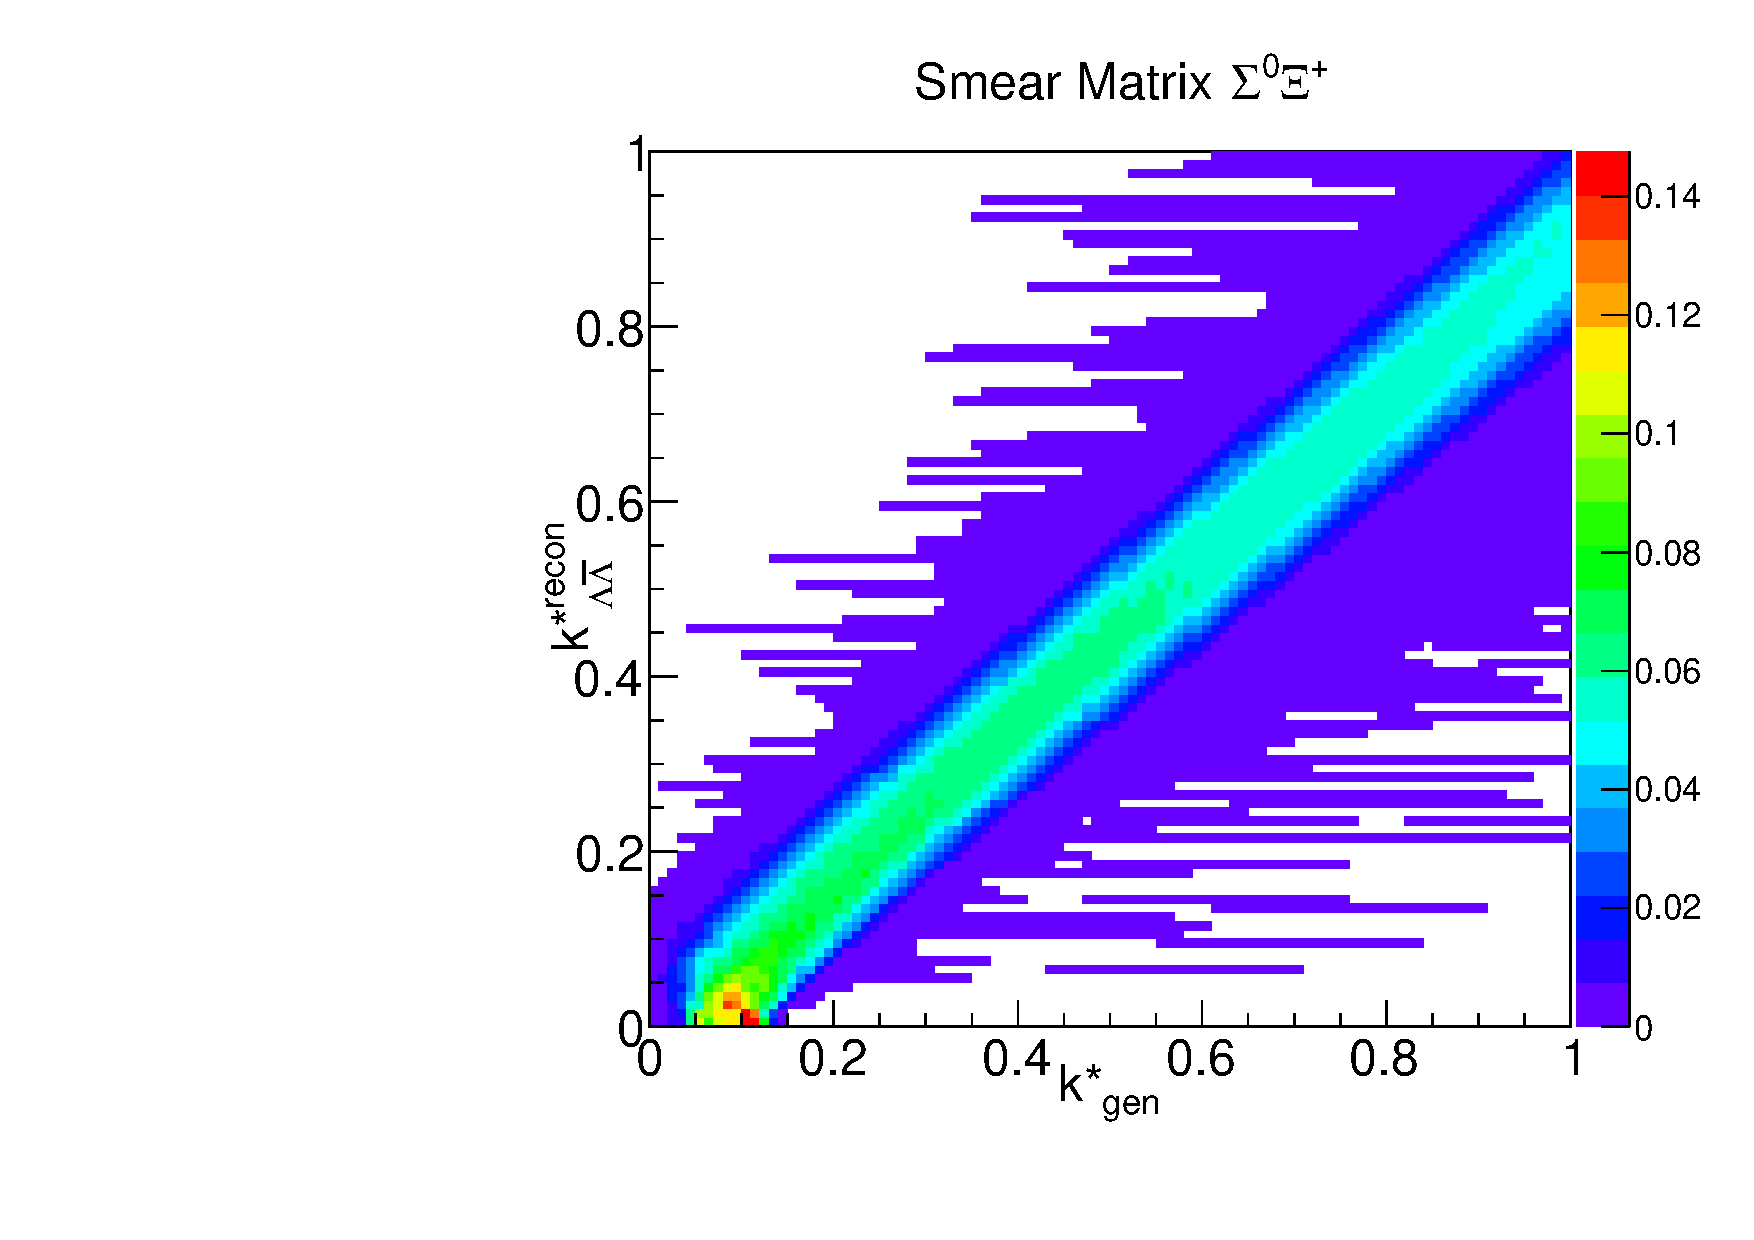
\includegraphics[width=18pc]{Figures/SmearMatrices/2016-7-19-SmearMatrixSigmaXiCNormLA.pdf}
\end{minipage}\hspace{2pc}
\begin{minipage}{18pc}
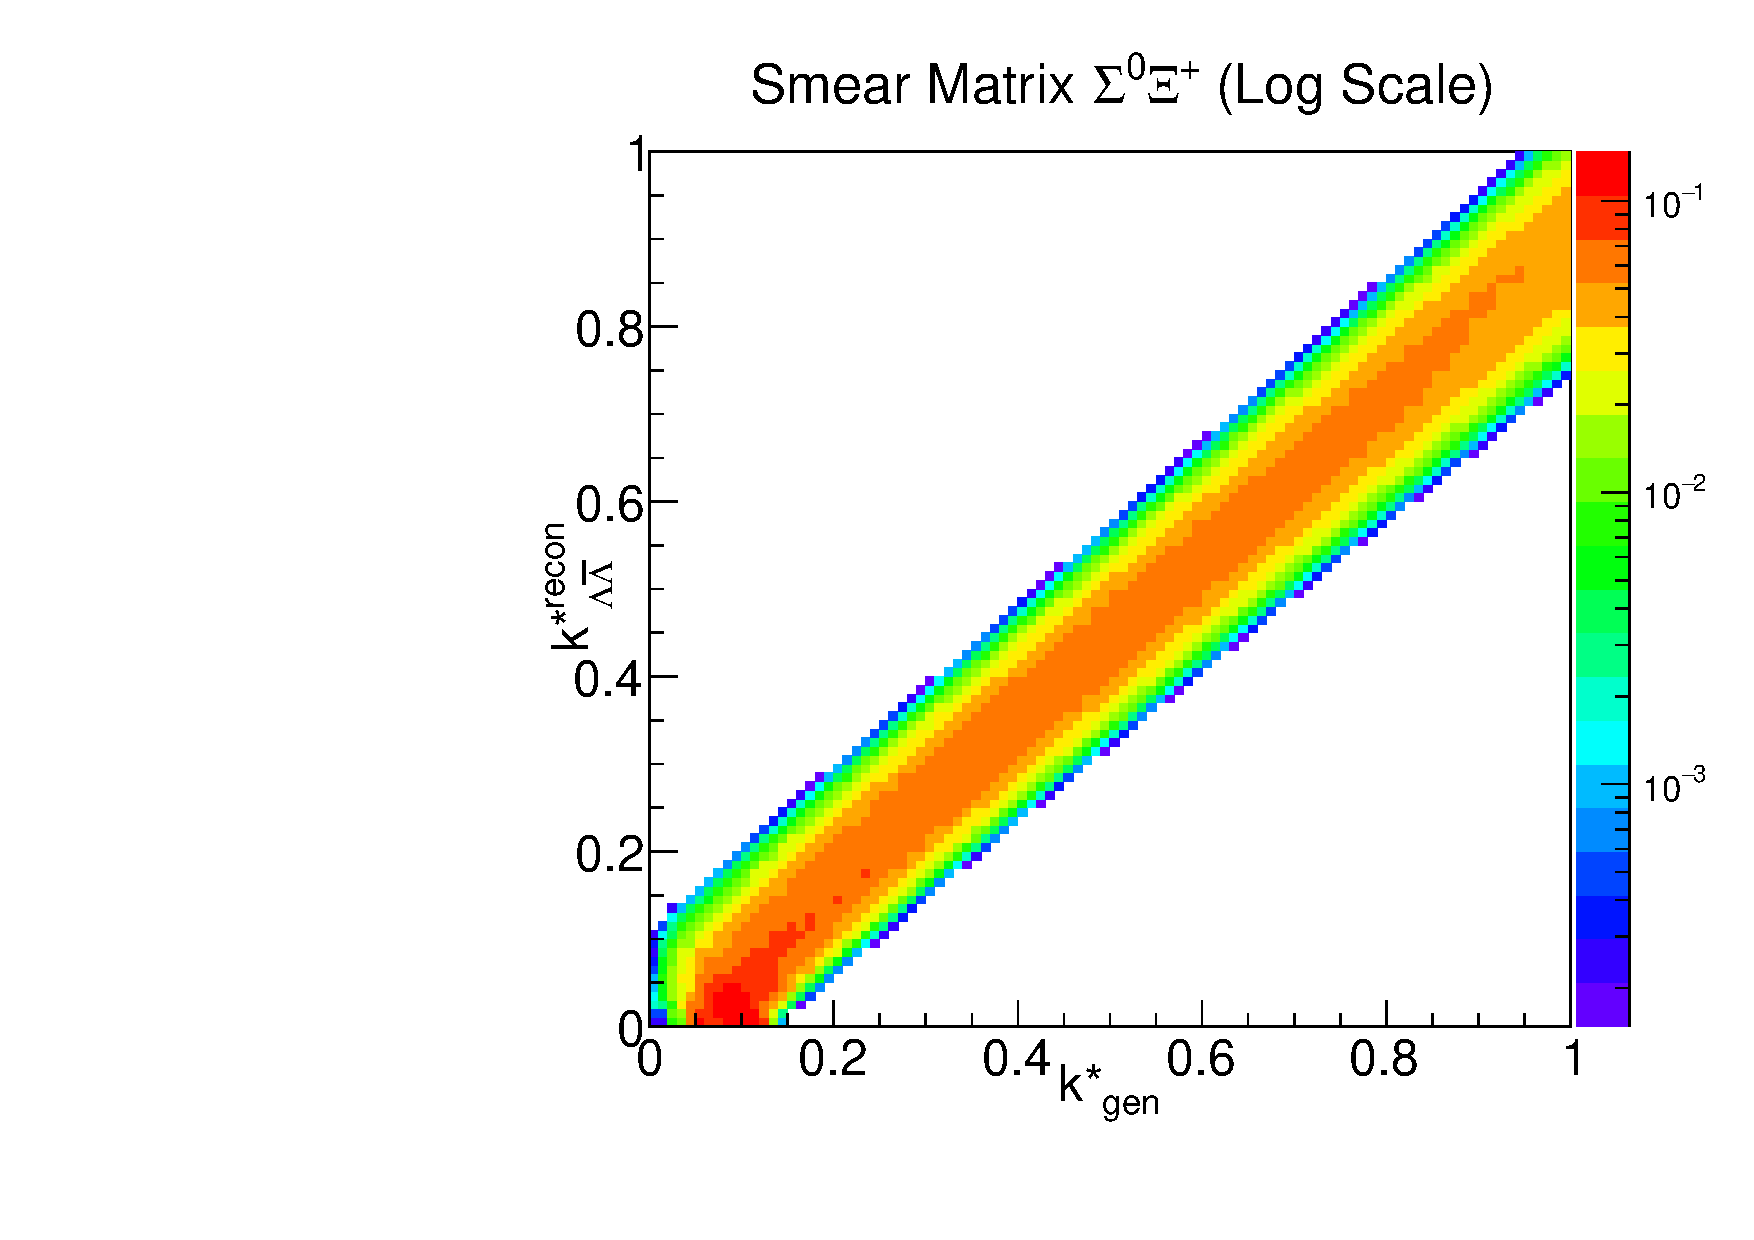
\includegraphics[width=18pc]{Figures/SmearMatrices/2016-7-19-SmearMatrixSigmaXiCNormLALog.pdf}
\end{minipage} 
\caption[Smear matrix -- $\Sigma^0\Xi^{+}$ and $\bar{\Sigma}^0\Xi^{-}$]{
Smear matrix for $\Sigma^0\Xi^{+}$ and $\bar{\Sigma}^0\Xi^{-}$, which accounts for both residual correlation and momentum resolution smearing. This matrix can be used to correct the theoretical correlation function so that the fit has the same smearing as the data.
}
\end{figure}

\begin{figure}[h]
\begin{minipage}{18pc}
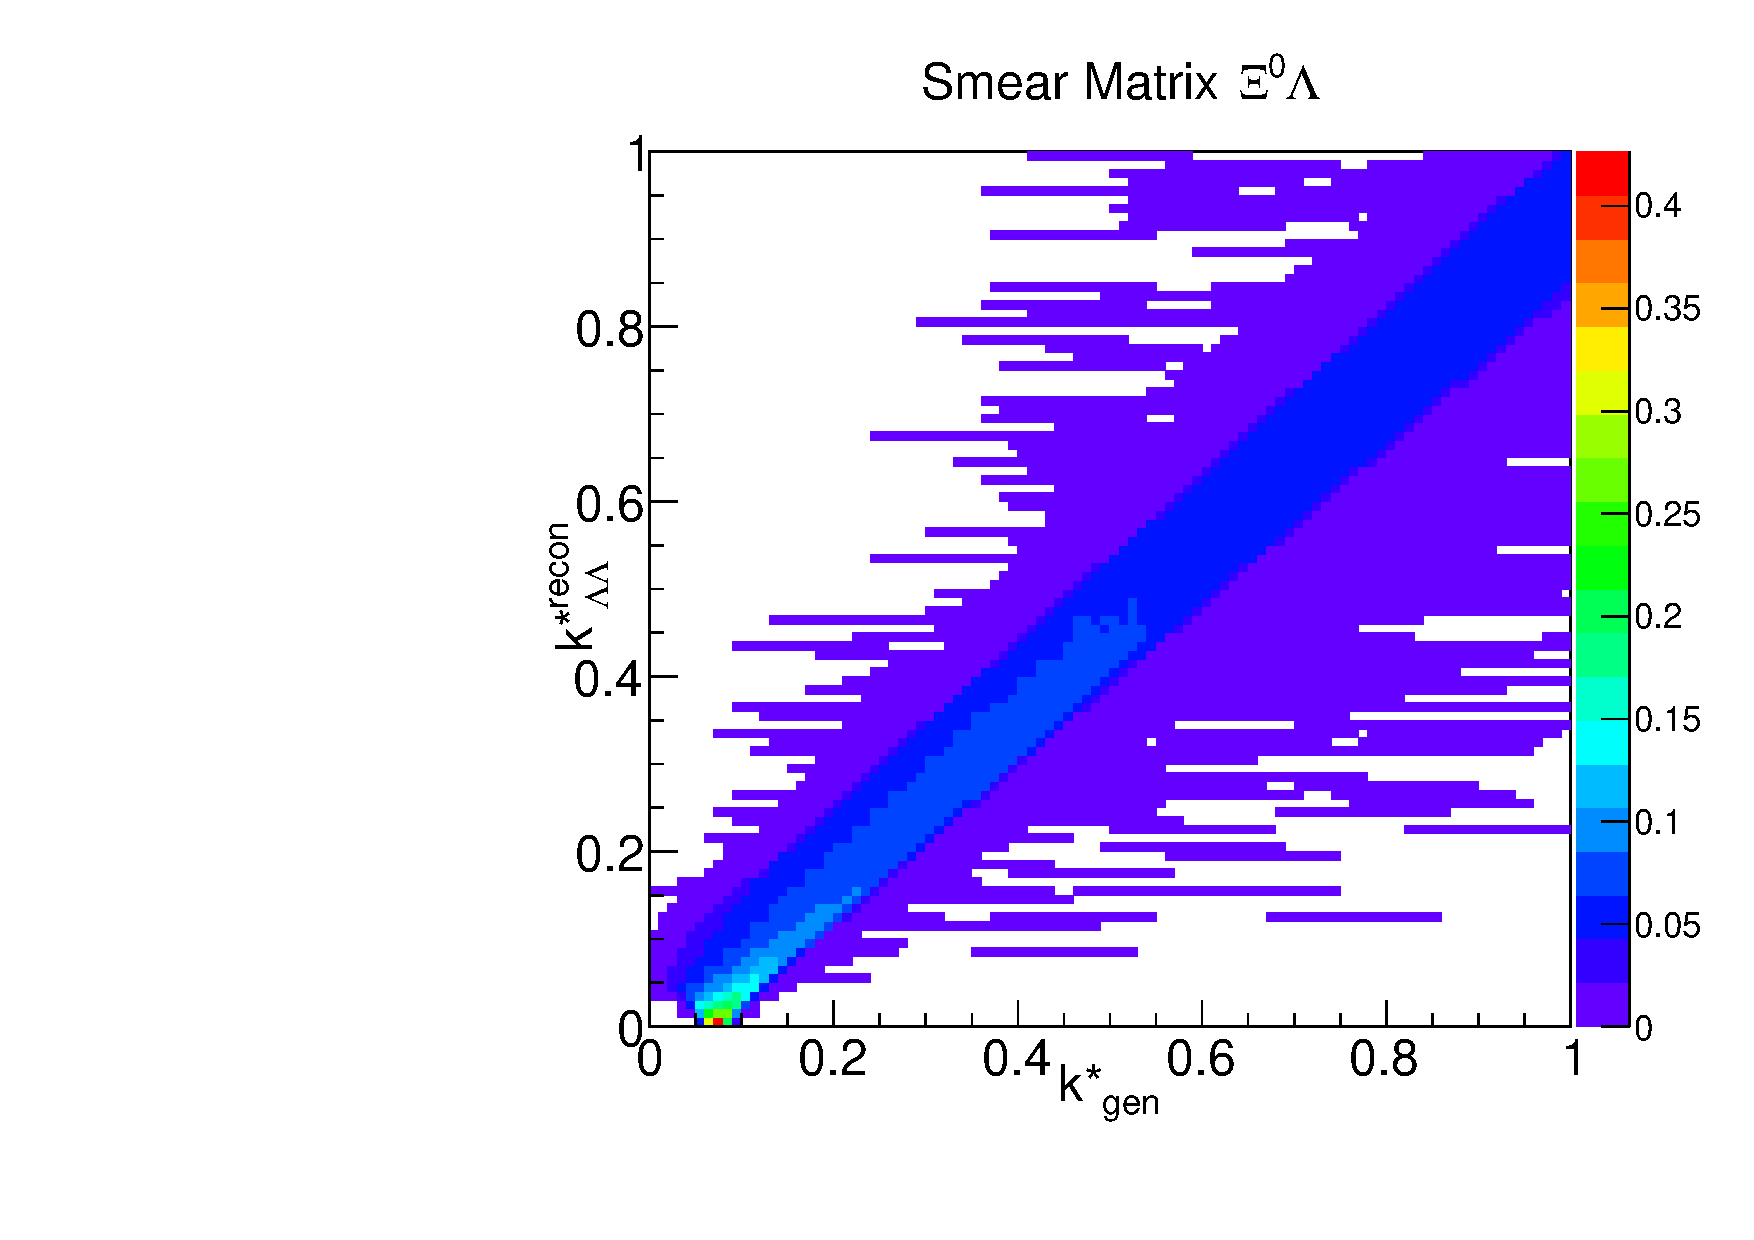
\includegraphics[width=18pc]{Figures/SmearMatrices/2016-7-19-SmearMatrixXi0LambdaNormLLAA.pdf}
\end{minipage}\hspace{2pc}
\begin{minipage}{18pc}
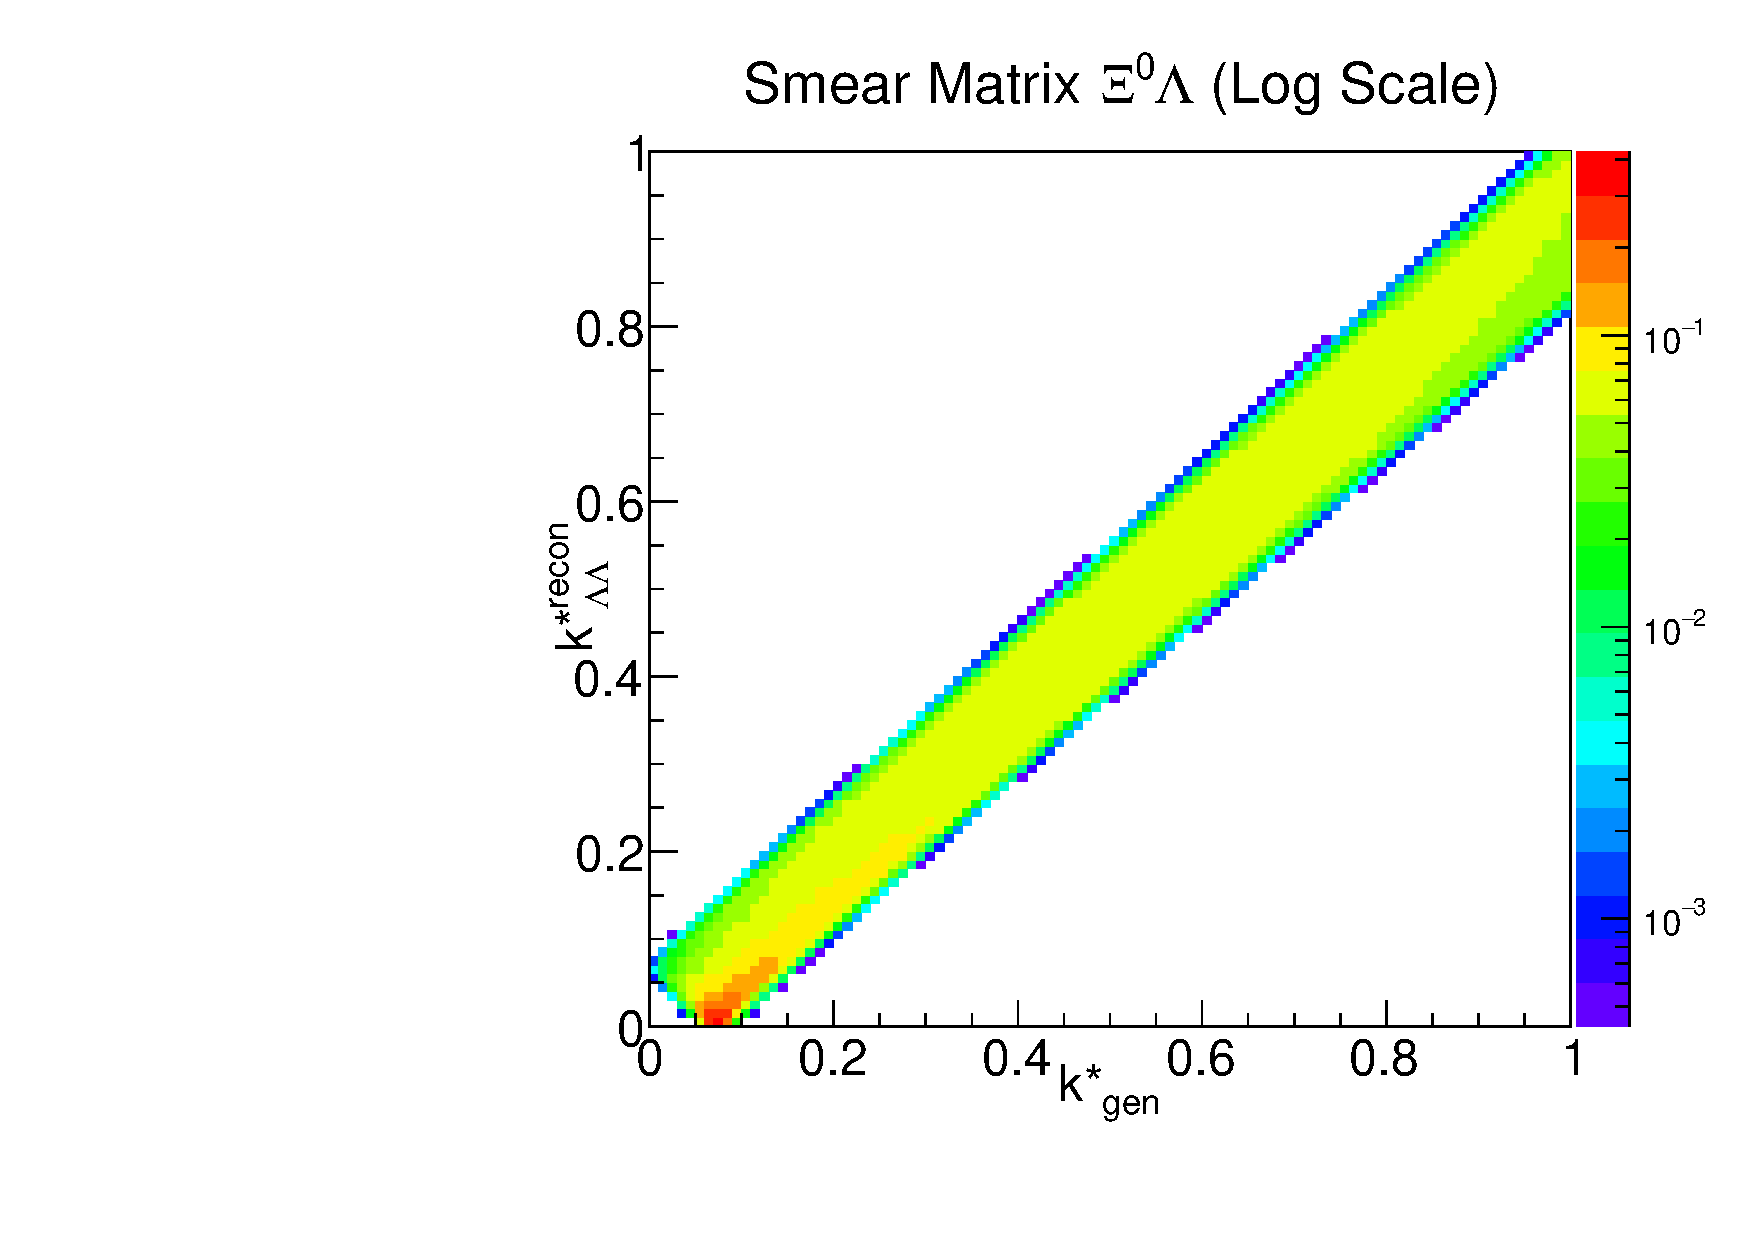
\includegraphics[width=18pc]{Figures/SmearMatrices/2016-7-19-SmearMatrixXi0LambdaNormLLAALog.pdf}
\end{minipage} 
\caption[Smear matrix -- $\Xi^0\Lambda$ and $\bar{\Xi}^0\bar{\Lambda}$]{
Smear matrix for $\Xi^0\Lambda$ and $\bar{\Xi}^0\bar{\Lambda}$, which accounts for both residual correlation and momentum resolution smearing. This matrix can be used to correct the theoretical correlation function so that the fit has the same smearing as the data.
}
\end{figure}

\begin{figure}[h]
\begin{minipage}{18pc}
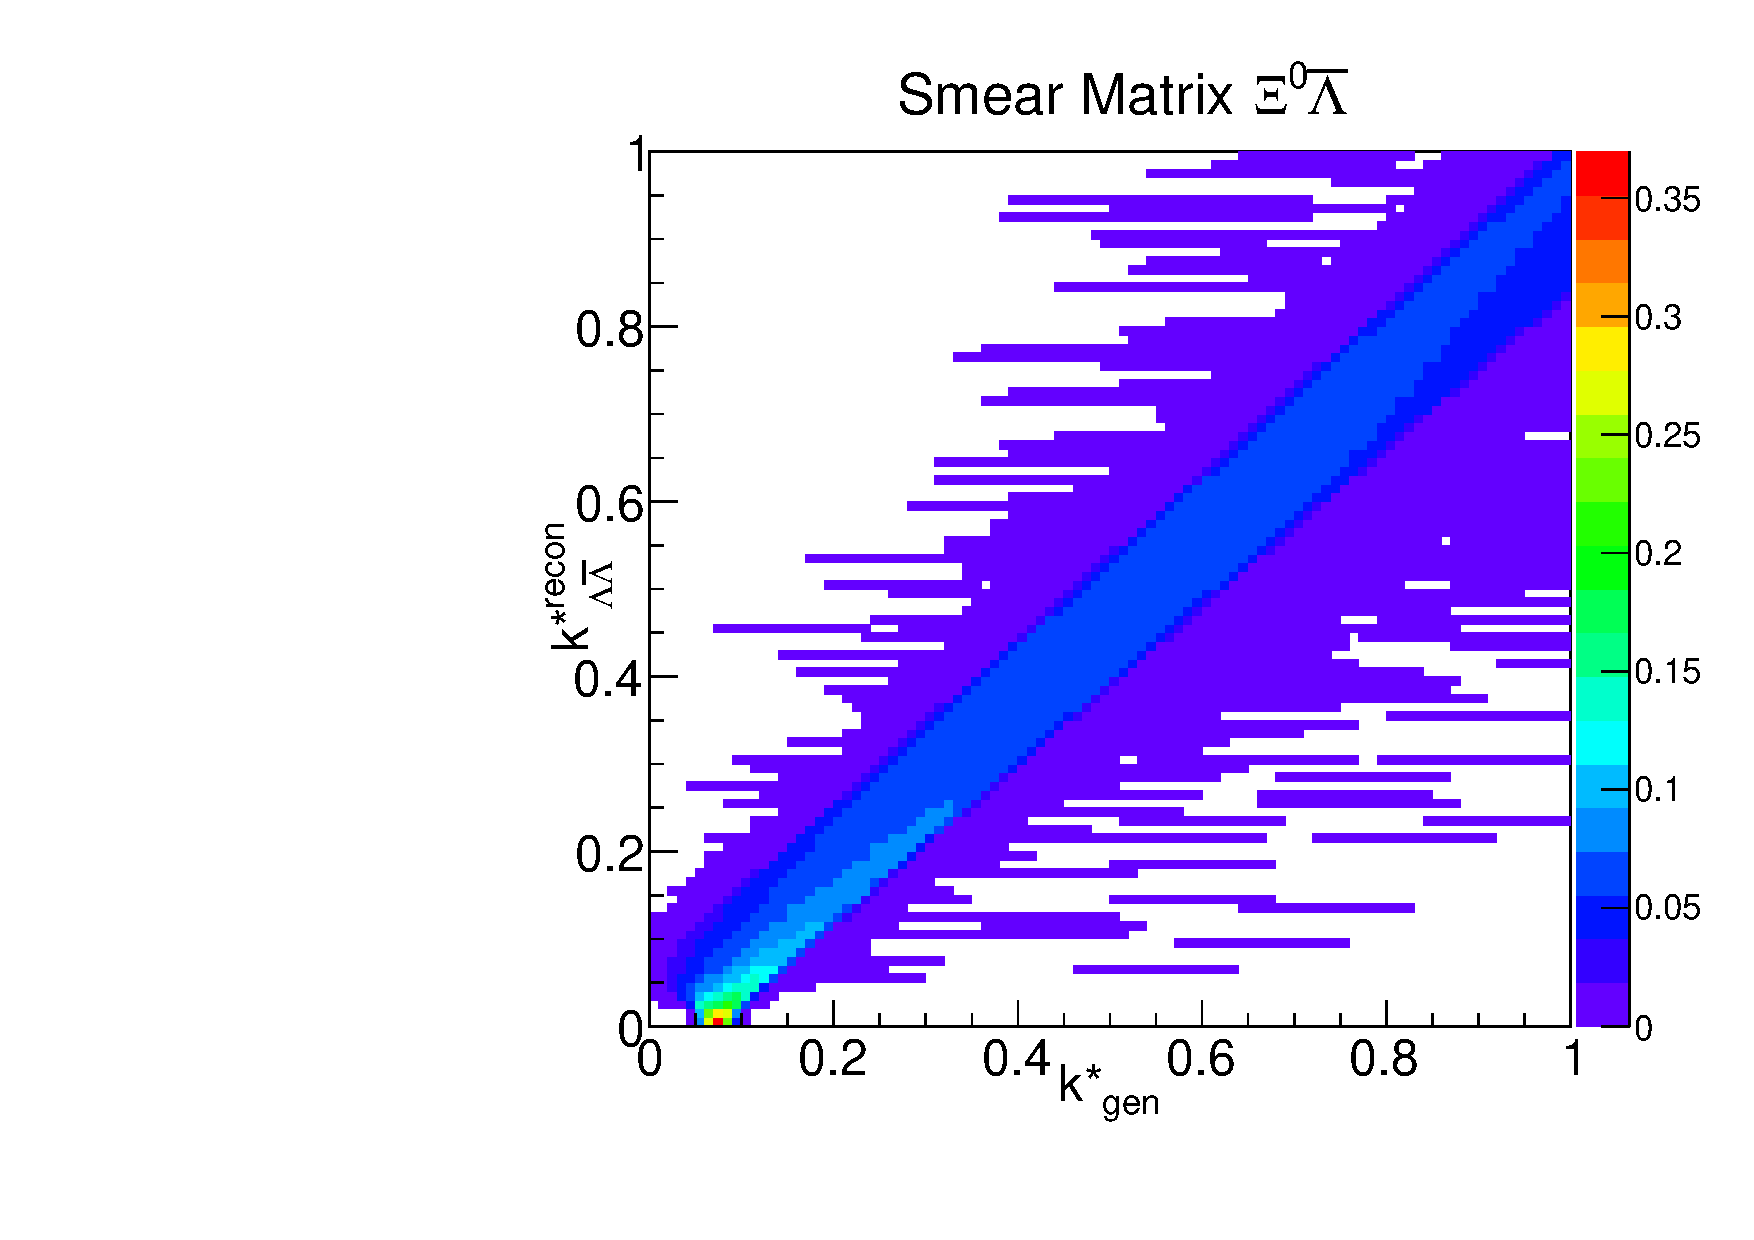
\includegraphics[width=18pc]{Figures/SmearMatrices/2016-7-19-SmearMatrixXi0LambdaNormLA.pdf}
\end{minipage}\hspace{2pc}
\begin{minipage}{18pc}
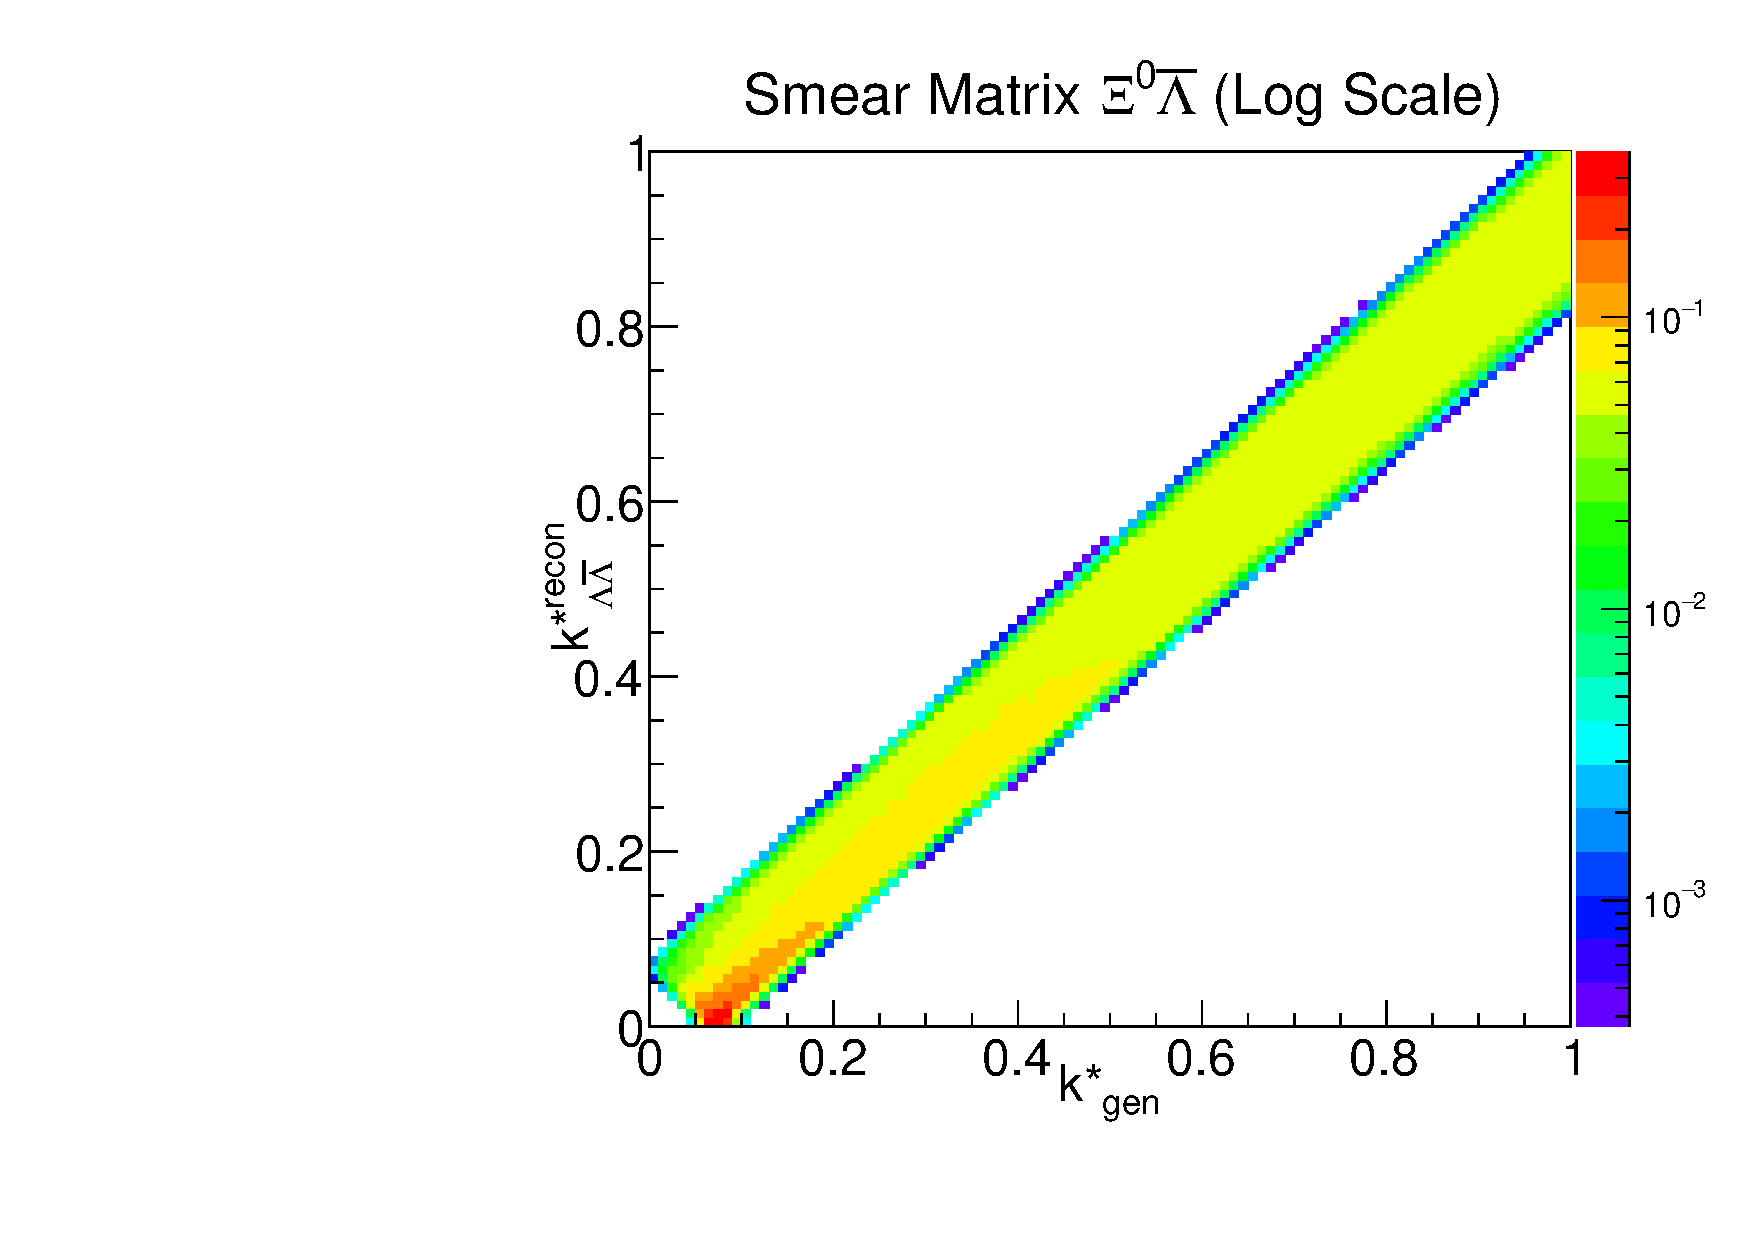
\includegraphics[width=18pc]{Figures/SmearMatrices/2016-7-19-SmearMatrixXi0LambdaNormLALog.pdf}
\end{minipage} 
\caption[Smear matrix -- $\Xi^0\bar{\Lambda}$ and $\bar{\Xi}^0\Lambda$]{
Smear matrix for $\Xi^0\bar{\Lambda}$ and $\bar{\Xi}^0\Lambda$, which accounts for both residual correlation and momentum resolution smearing. This matrix can be used to correct the theoretical correlation function so that the fit has the same smearing as the data.
}
\end{figure}

\begin{figure}[h]
\begin{minipage}{18pc}
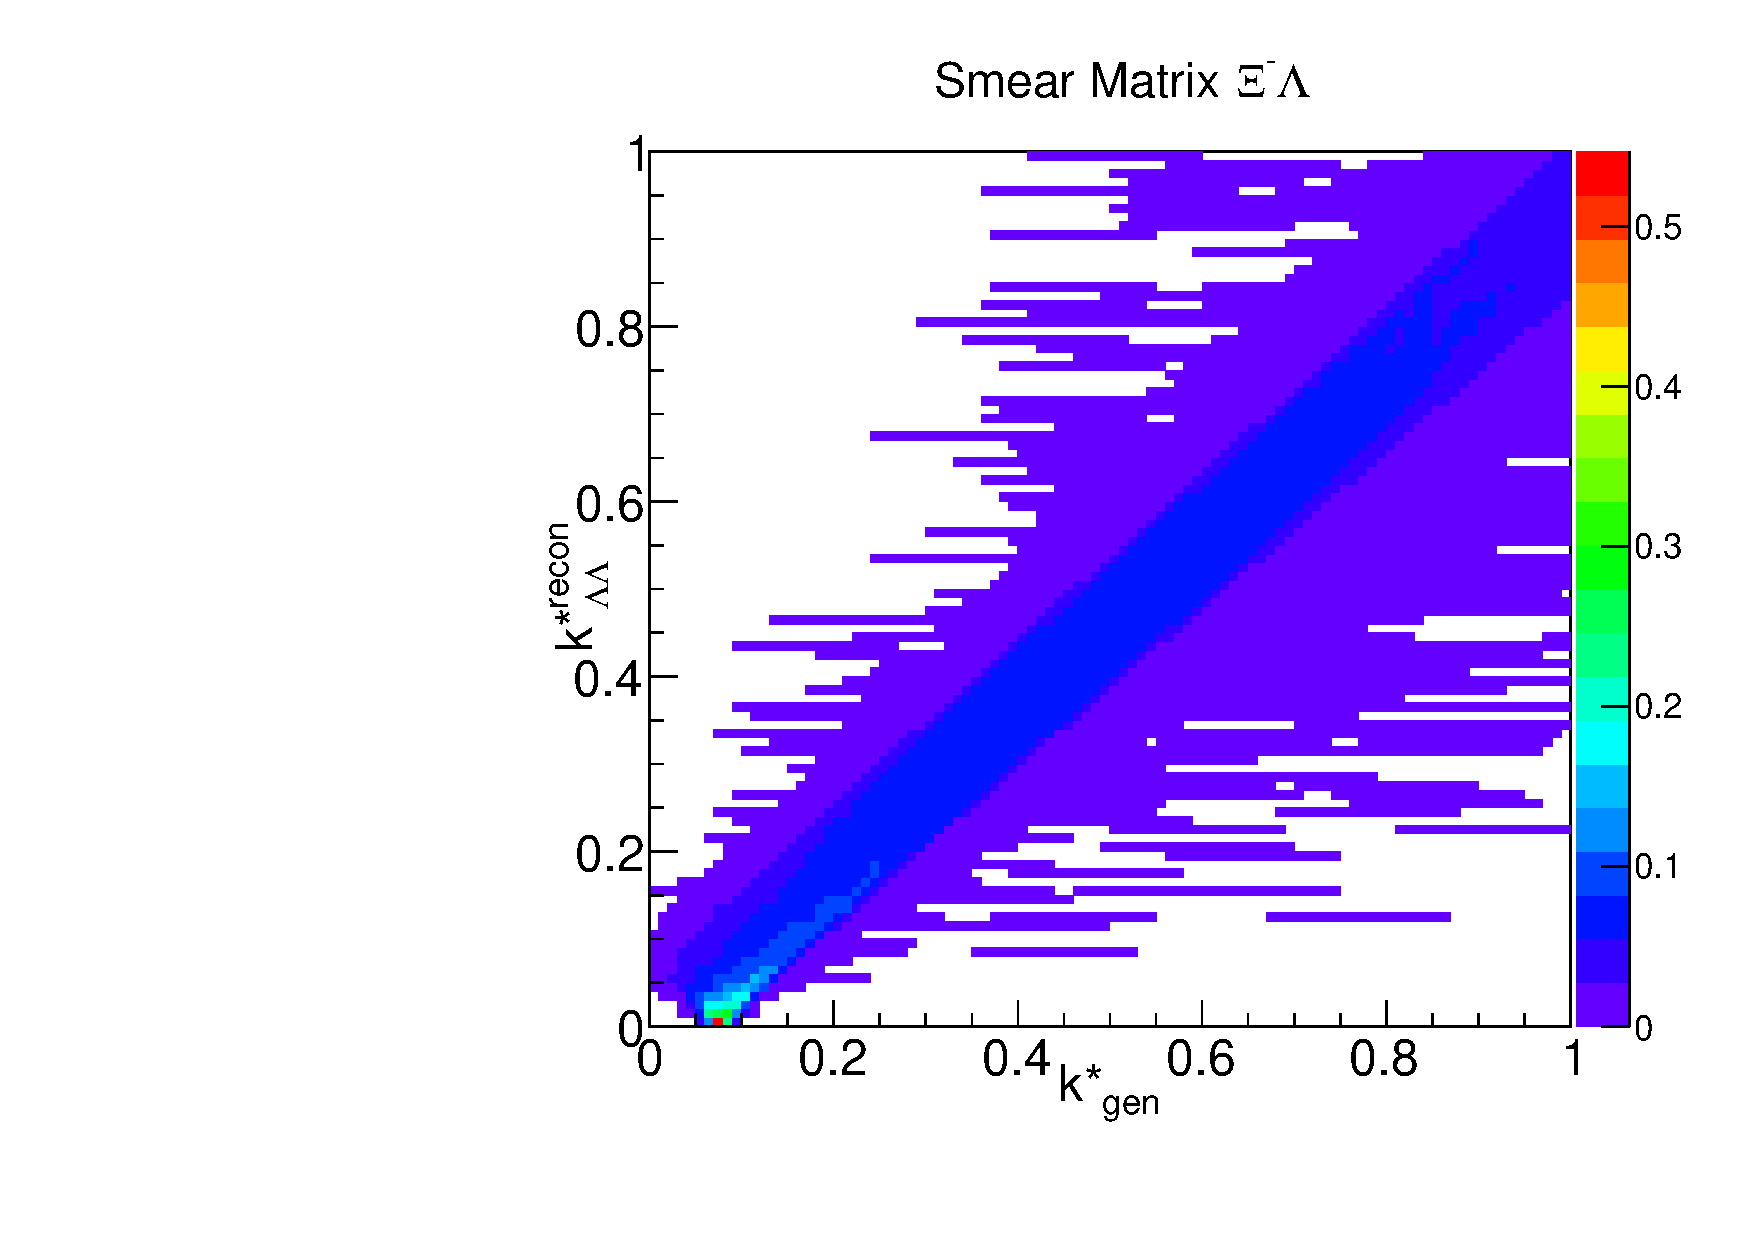
\includegraphics[width=18pc]{Figures/SmearMatrices/2016-7-19-SmearMatrixXiCLambdaNormLLAA.pdf}
\end{minipage}\hspace{2pc}
\begin{minipage}{18pc}
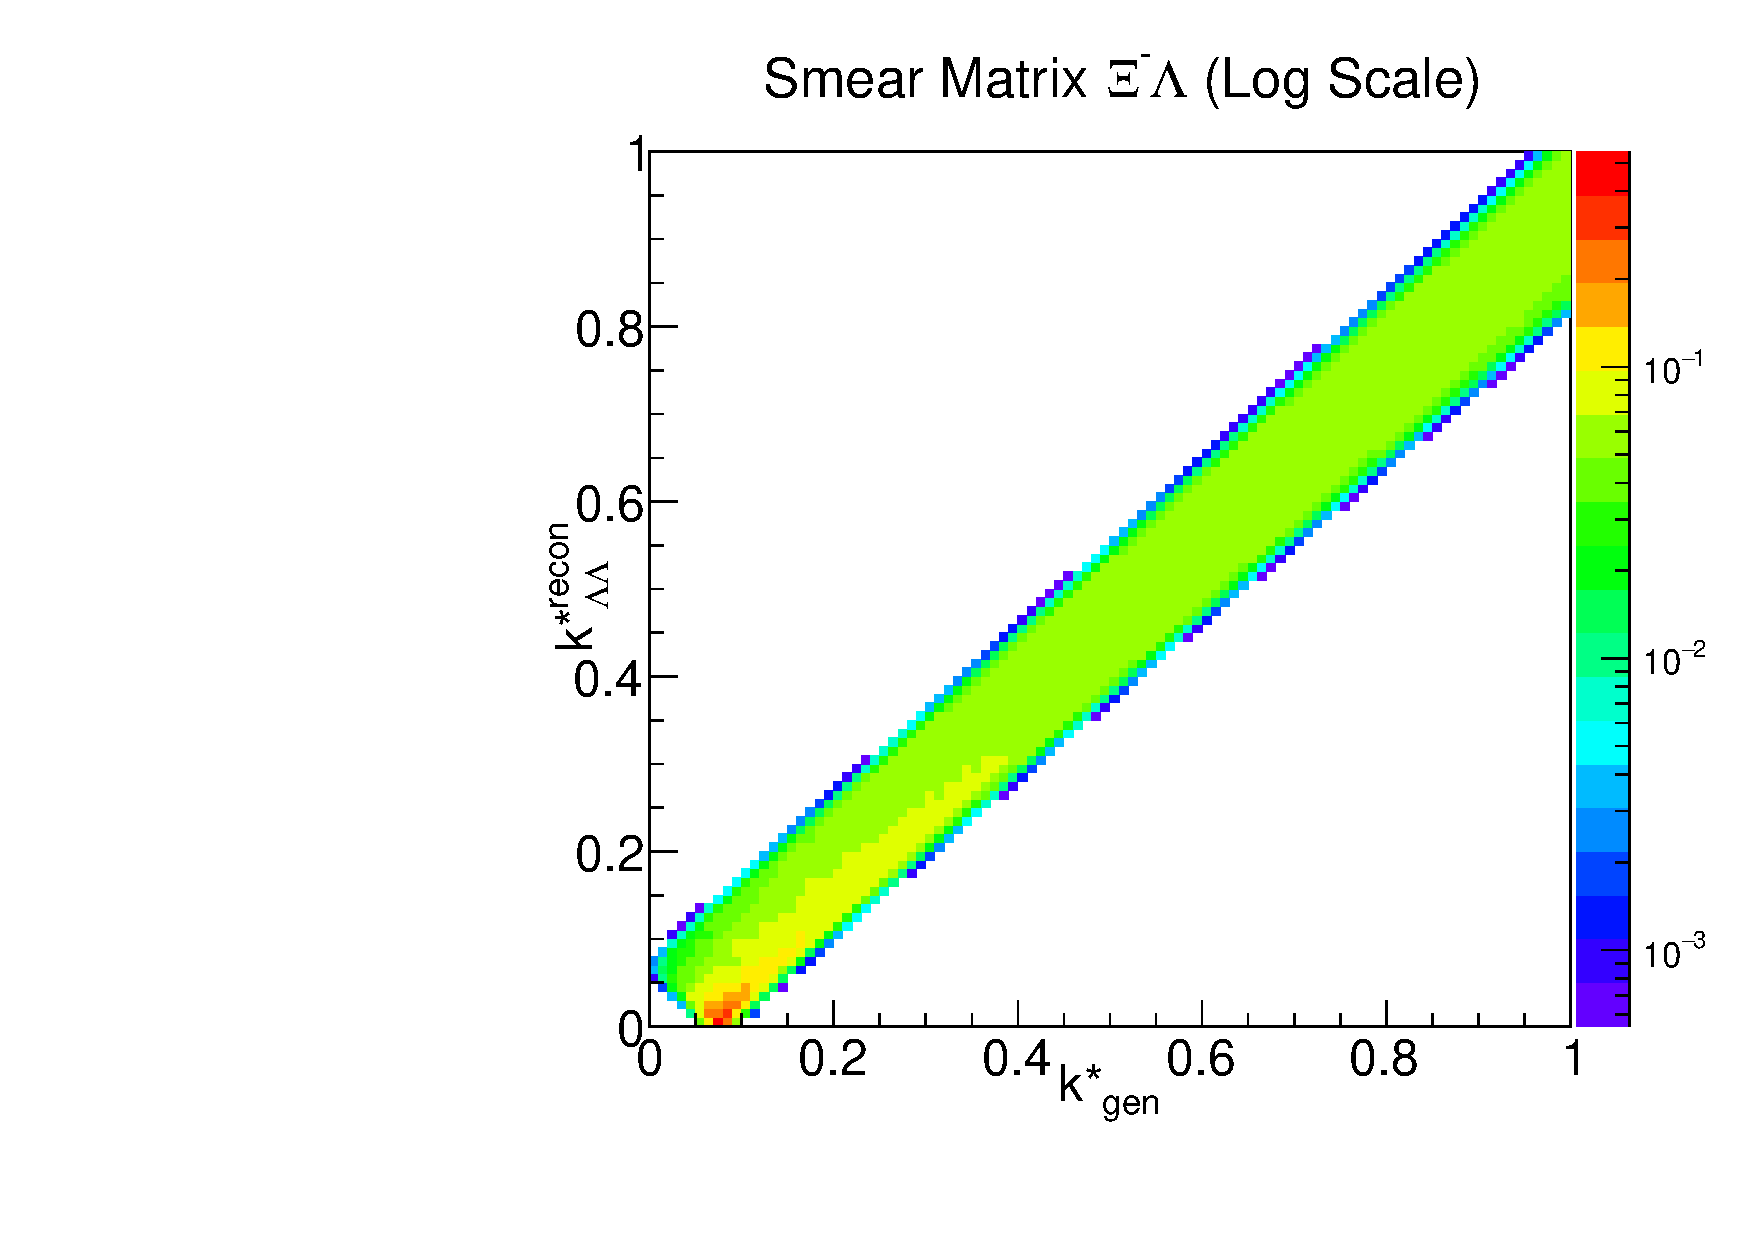
\includegraphics[width=18pc]{Figures/SmearMatrices/2016-7-19-SmearMatrixXiCLambdaNormLLAALog.pdf}
\end{minipage} 
\caption[Smear matrix -- $\Xi^{-}\Lambda$ and $\Xi^{+}\bar{\Lambda}$]{
Smear matrix for $\Xi^{-}\Lambda$ and $\Xi^{+}\bar{\Lambda}$, which accounts for both residual correlation and momentum resolution smearing. This matrix can be used to correct the theoretical correlation function so that the fit has the same smearing as the data.
}
\end{figure}

\begin{figure}[h]
\begin{minipage}{18pc}
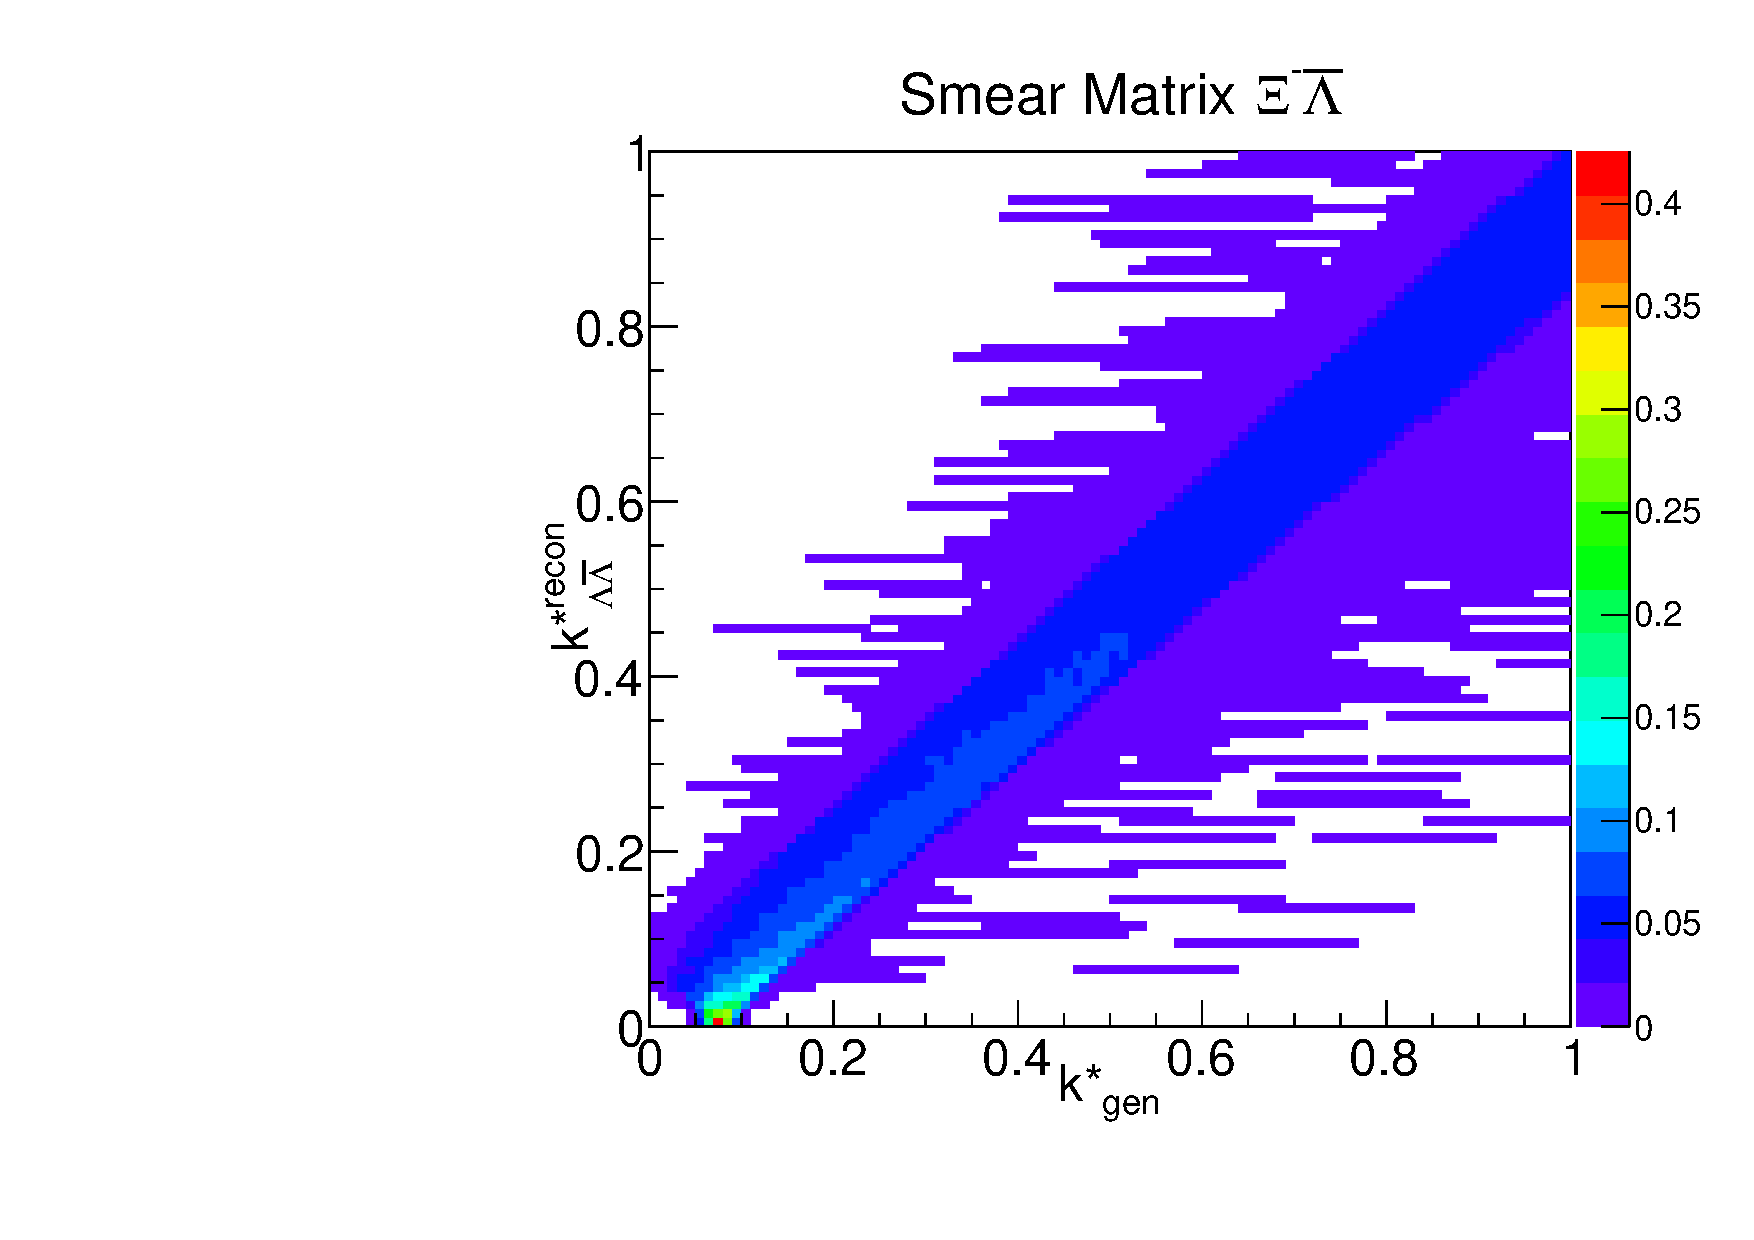
\includegraphics[width=18pc]{Figures/SmearMatrices/2016-7-19-SmearMatrixXiCLambdaNormLA.pdf}
\end{minipage}\hspace{2pc}
\begin{minipage}{18pc}
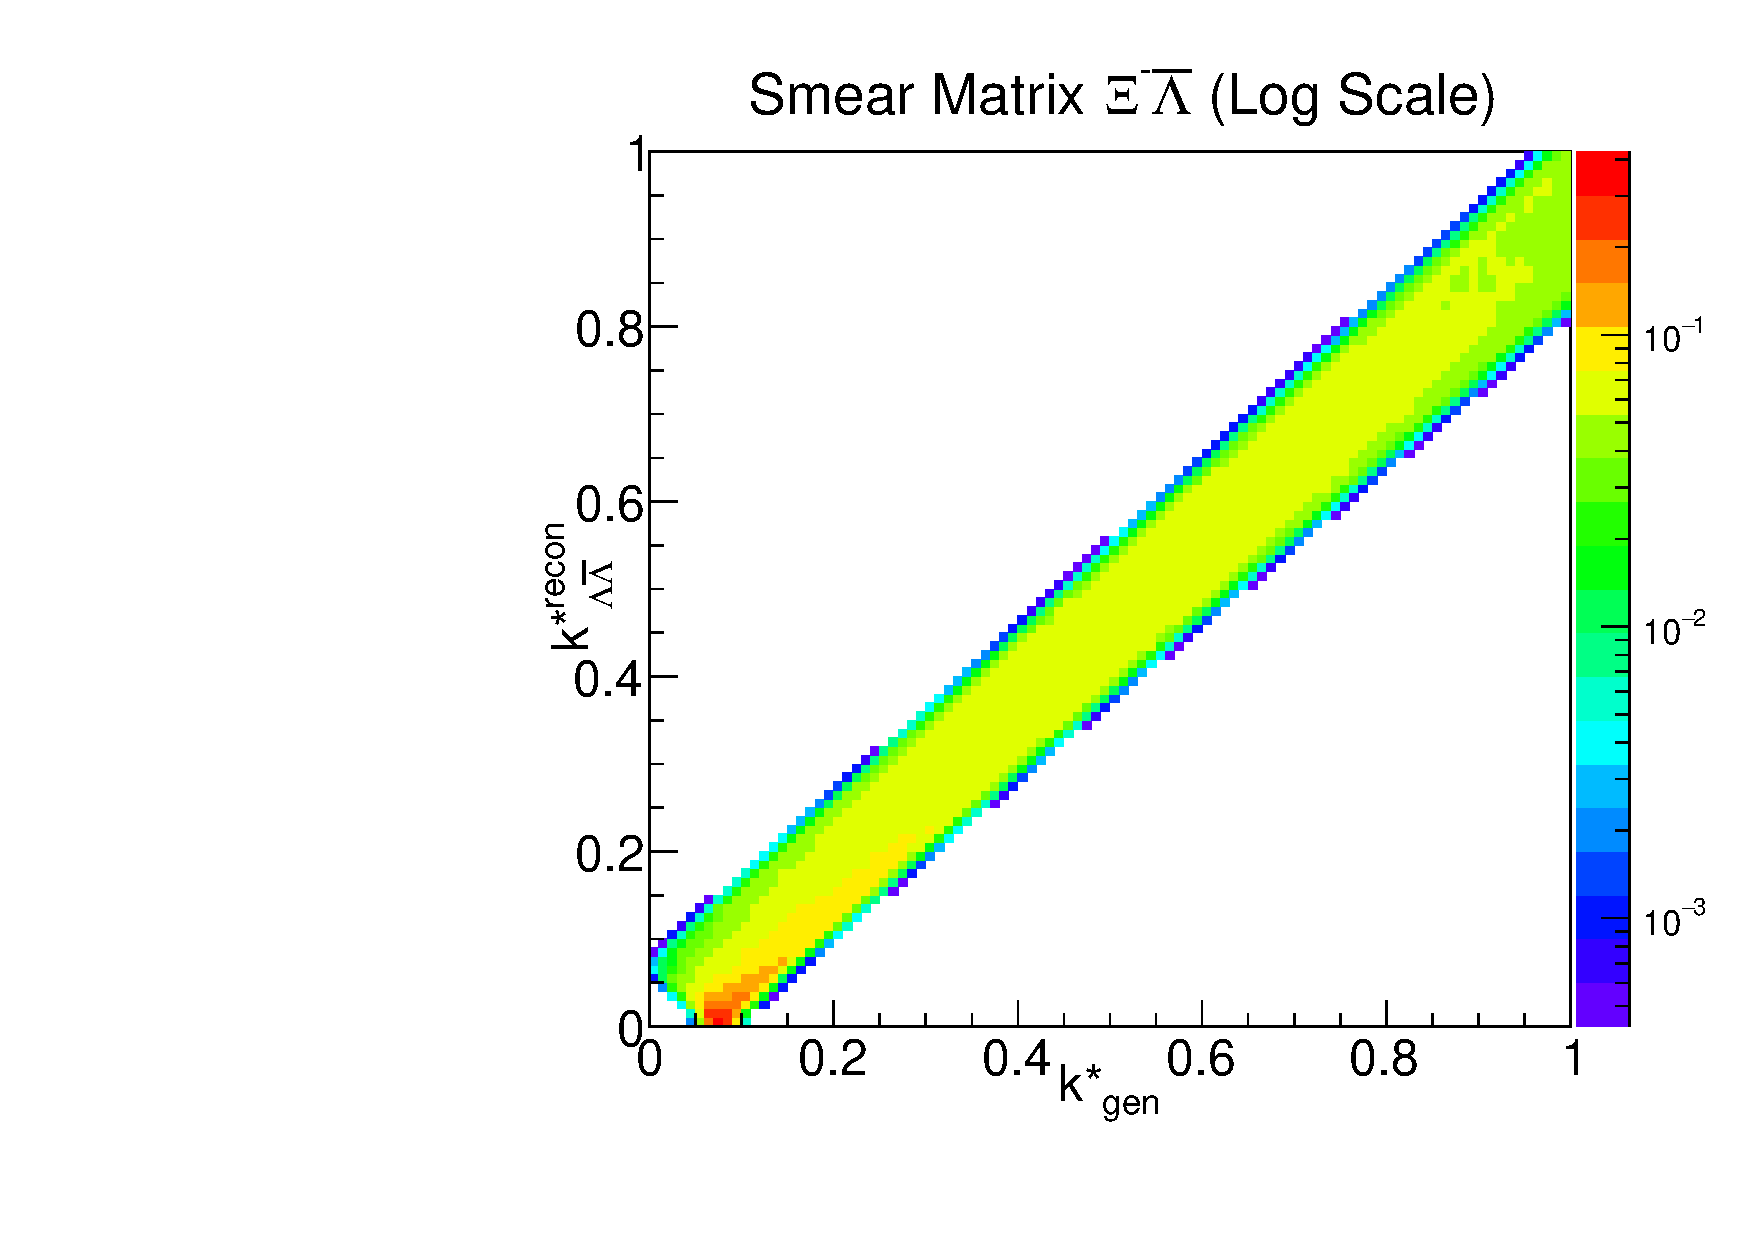
\includegraphics[width=18pc]{Figures/SmearMatrices/2016-7-19-SmearMatrixXiCLambdaNormLALog.pdf}
\end{minipage} 
\caption[Smear matrix -- $\Xi^{-}\bar{\Lambda}$ and $\Xi^{+}\Lambda$]{
Smear matrix for $\Xi^{-}\bar{\Lambda}$ and $\Xi^{+}\Lambda$, which accounts for both residual correlation and momentum resolution smearing. This matrix can be used to correct the theoretical correlation function so that the fit has the same smearing as the data.
}
\end{figure}

\begin{figure}[h]
\begin{minipage}{18pc}
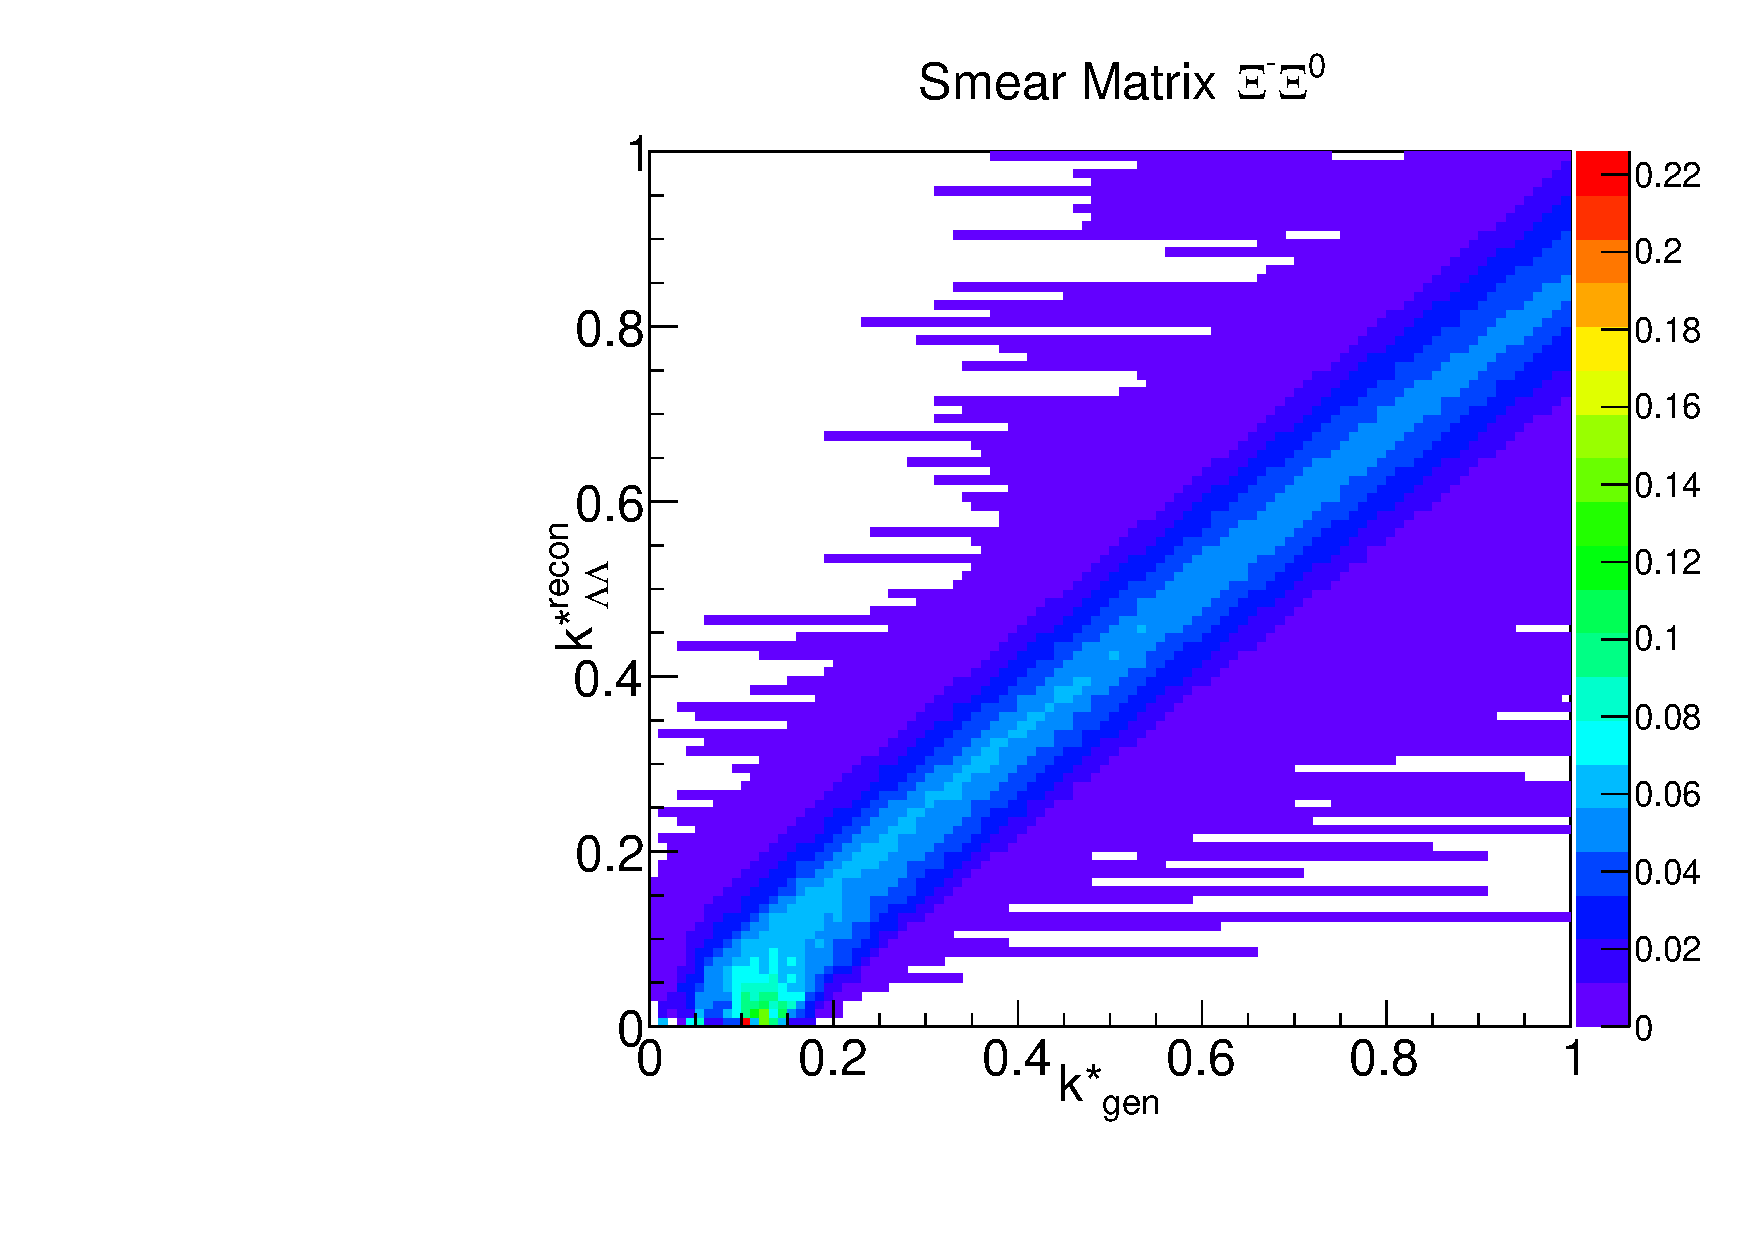
\includegraphics[width=18pc]{Figures/SmearMatrices/2016-7-19-SmearMatrixXiCXi0NormLLAA.pdf}
\end{minipage}\hspace{2pc}
\begin{minipage}{18pc}
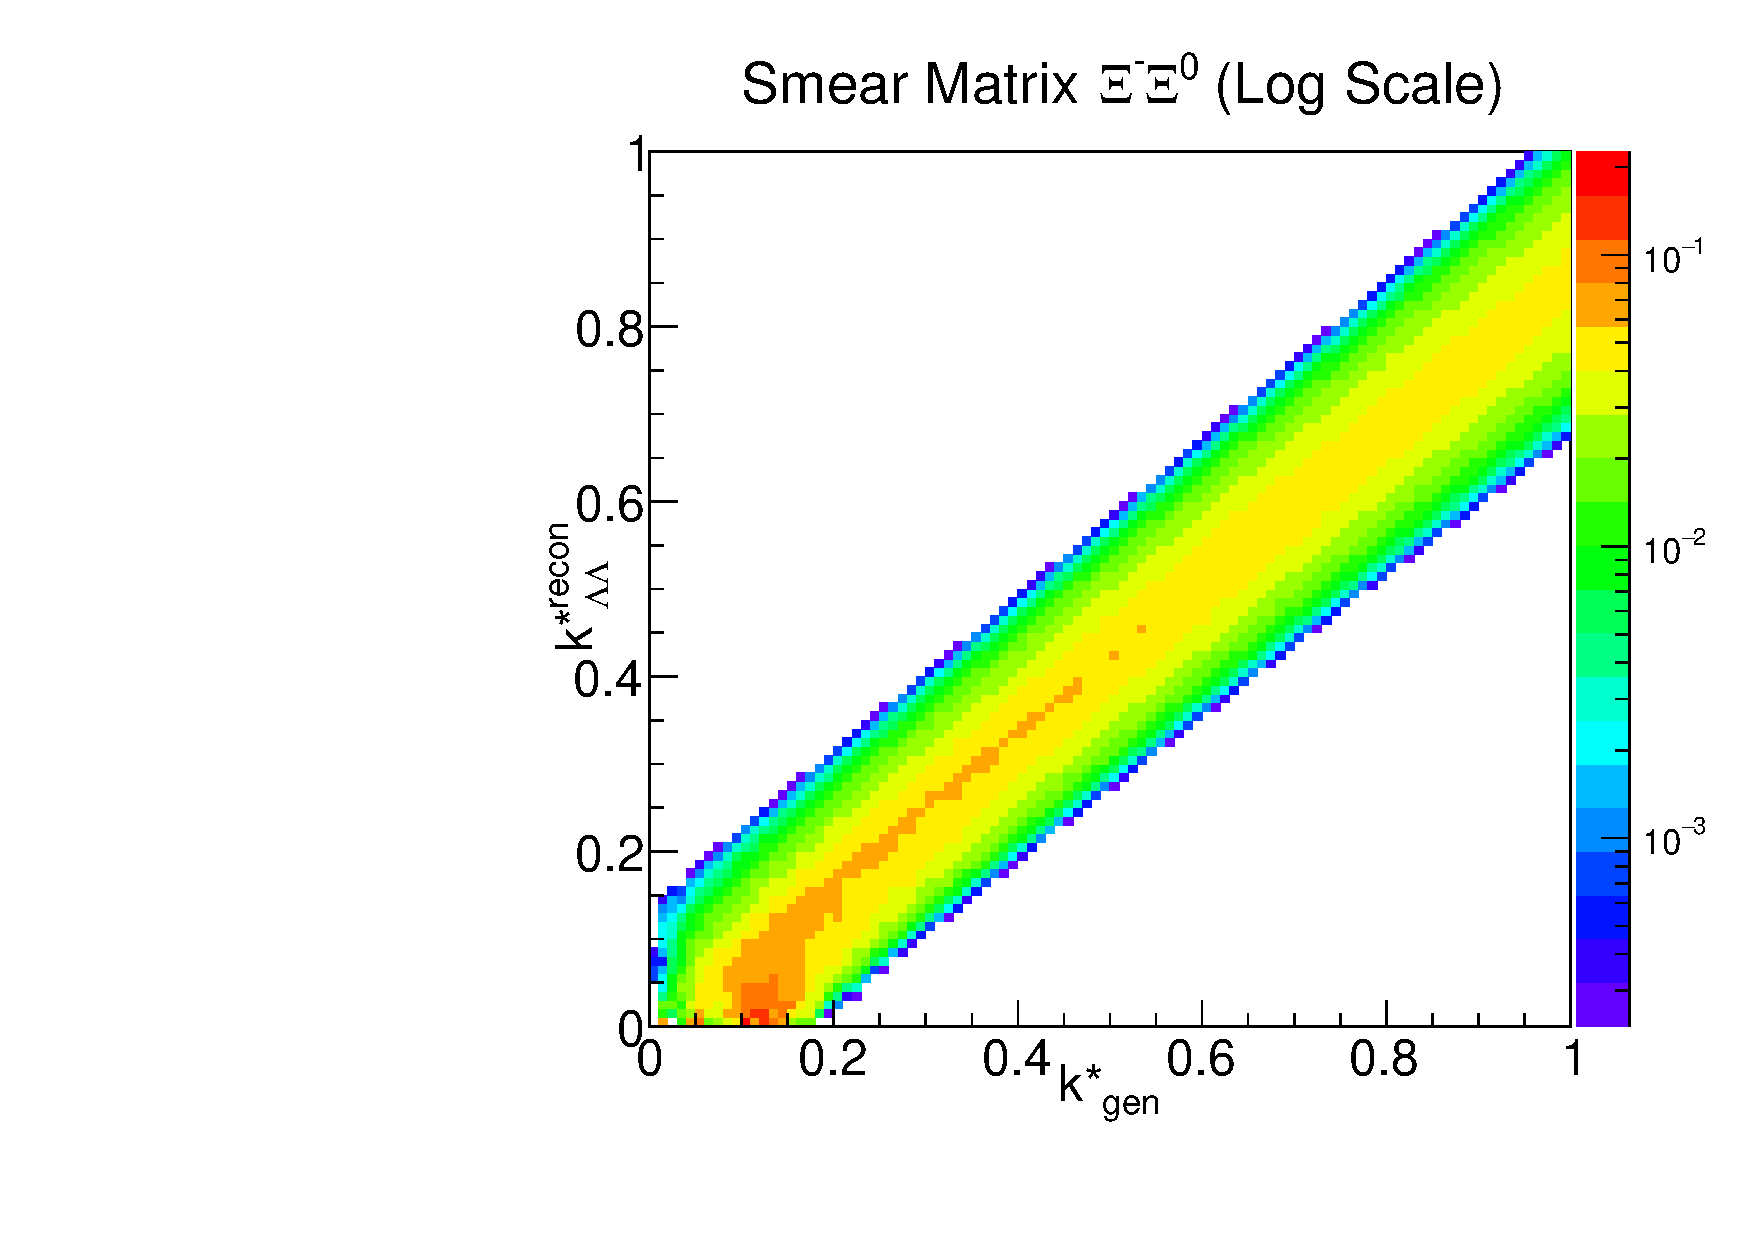
\includegraphics[width=18pc]{Figures/SmearMatrices/2016-7-19-SmearMatrixXiCXi0NormLLAALog.pdf}
\end{minipage} 
\caption[Smear matrix -- $\Xi^{-}\Xi^0$ and $\Xi^{+}\bar{\Xi}^0$]{
Smear matrix for $\Xi^{-}\Xi^0$ and $\Xi^{+}\bar{\Xi}^0$, which accounts for both residual correlation and momentum resolution smearing. This matrix can be used to correct the theoretical correlation function so that the fit has the same smearing as the data.
}
\end{figure}

\begin{figure}[h]
\begin{minipage}{18pc}
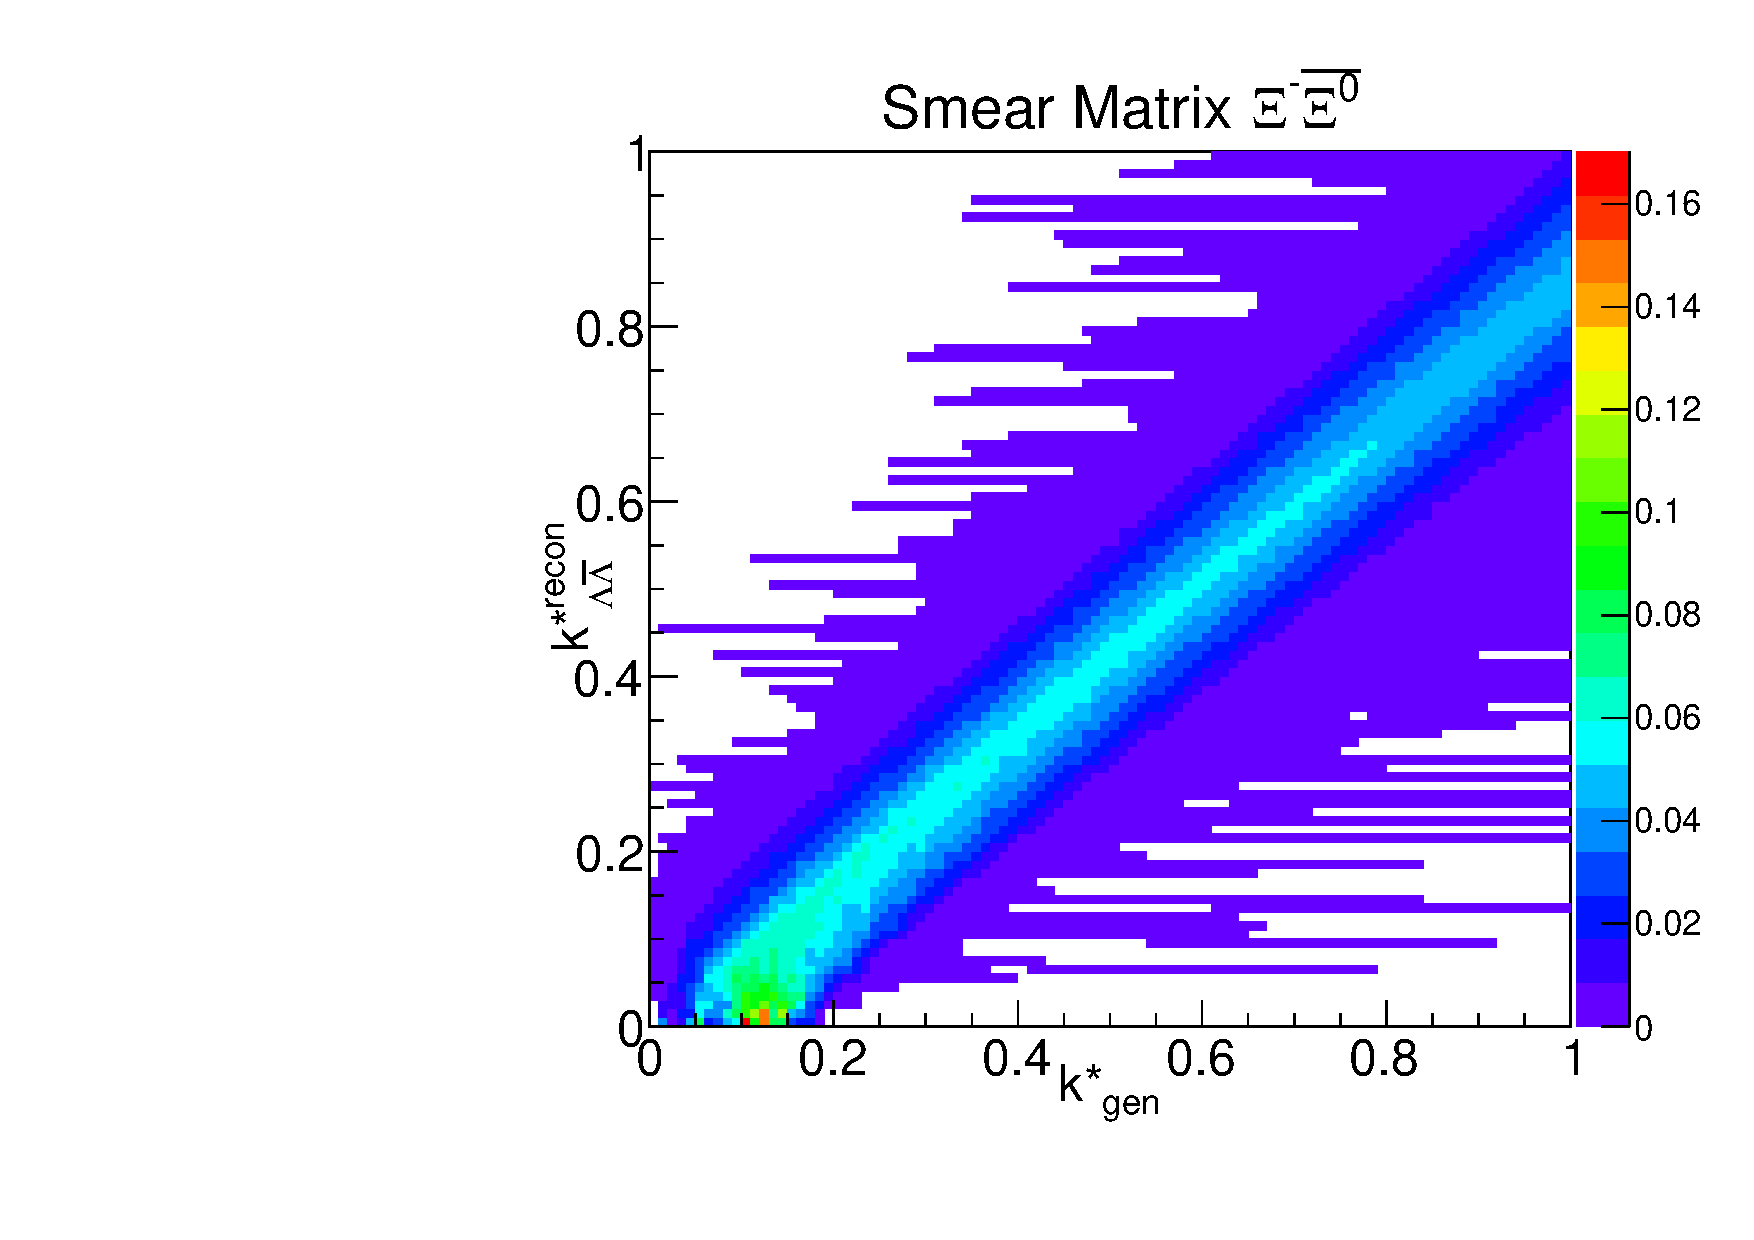
\includegraphics[width=18pc]{Figures/SmearMatrices/2016-7-19-SmearMatrixXiCXi0NormLA.pdf}
\end{minipage}\hspace{2pc}
\begin{minipage}{18pc}
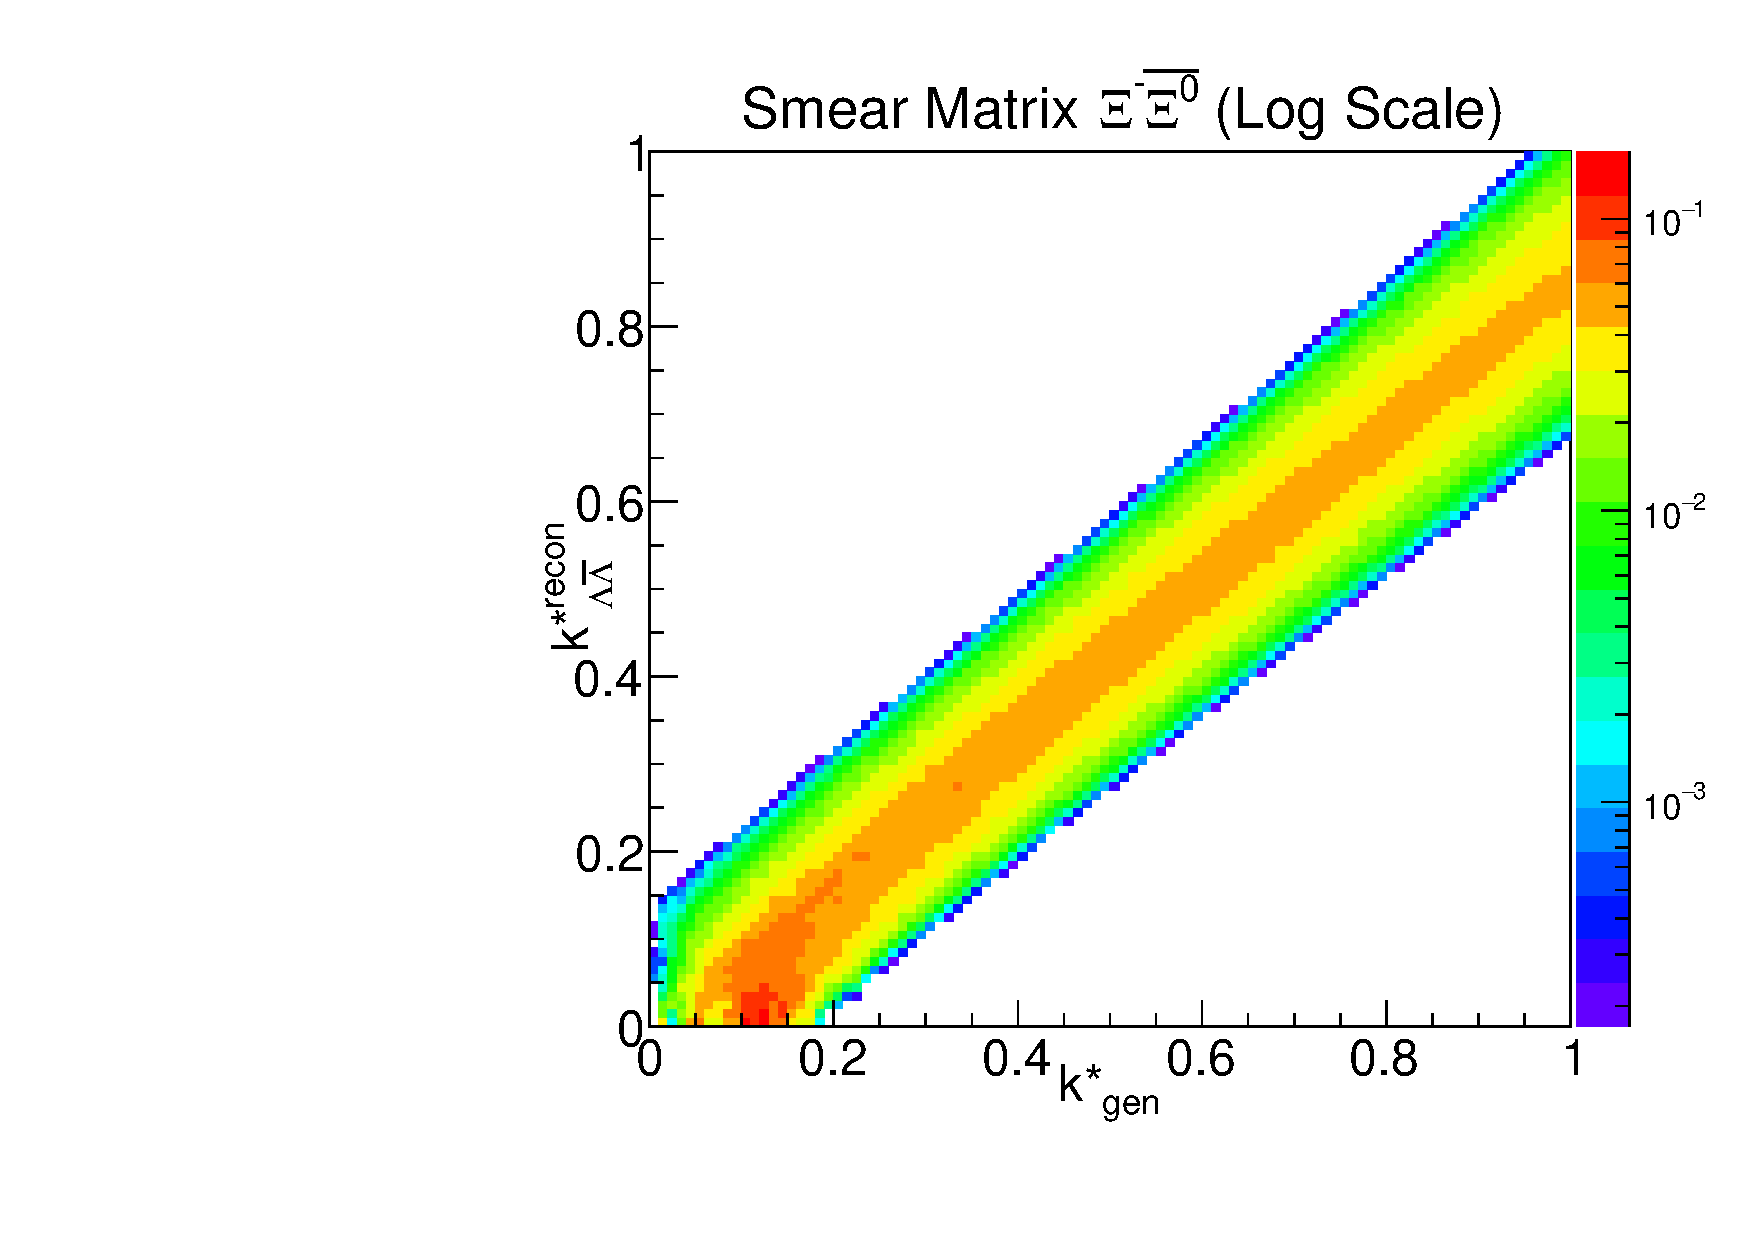
\includegraphics[width=18pc]{Figures/SmearMatrices/2016-7-19-SmearMatrixXiCXi0NormLALog.pdf}
\end{minipage} 
\caption[Smear matrix -- $\Xi^{-}\bar{\Xi}^0$ and $\Xi^{+}\Xi^0$]{\label{fig:SmearXiCXi0LA}
Smear matrix for $\Xi^{-}\bar{\Xi}^0$ and $\Xi^{+}\Xi^0$, which accounts for both residual correlation and momentum resolution smearing. This matrix can be used to correct the theoretical correlation function so that the fit has the same smearing as the data.
}
\end{figure}


\subsubsection{Implementation in fit}

When calculating the fit function, the contribution from the primary correlation function $C_{\Lambda\Lambda}(k^*_{\Lambda\Lambda})$ and each residual correlation  ($C_{ij}(k^*_{ij})$) is first calculated according to Eqn.\ \ref{eq:Lednicky}.
Then each contribution is smeared with its own smear matrix via Eqn.\ \ref{eq:FullSmearing}.
Finally, each contribution is combined using the $\lambda$ weights according to Eqn. \ref{eq:Residual}.

 